\documentclass[11pt,a4paper,oneside]{book}
\usepackage[T1]{fontenc}
\usepackage{lmodern}
\usepackage[english]{babel}
\usepackage[a4paper,margin=2.4cm,top=2.6cm,bottom=2.6cm]{geometry}
\usepackage[english]{mugango-apostila}
\usepackage[hidelinks]{hyperref}

\DeclareUnicodeCharacter{26A0}{\textcolor{vermesc}{\textbf{\textsf{!}}}}
\DeclareUnicodeCharacter{FE0F}{}
\DeclareUnicodeCharacter{2192}{\ensuremath{\rightarrow}}
\DeclareUnicodeCharacter{2264}{\ensuremath{\leq}}
\DeclareUnicodeCharacter{2265}{\ensuremath{\geq}}
\DeclareUnicodeCharacter{2212}{\ensuremath{-}}
\DeclareUnicodeCharacter{0393}{\ensuremath{\Gamma}}
\DeclareUnicodeCharacter{03C1}{\ensuremath{\rho}}
\DeclareUnicodeCharacter{00D7}{\ensuremath{\times}}
\DeclareUnicodeCharacter{2248}{\ensuremath{\approx}}
\DeclareUnicodeCharacter{0394}{\ensuremath{\Delta}}

\graphicspath{{figs/}}

% ---- notation shared by every chapter (see BRIEF.md) ------------------------------
\newcommand{\rval}{r_{\mathrm{val}}}
\newcommand{\rnul}{r_{0}}
\newcommand{\rclaim}{r_{\mathrm{claim}}}
\newcommand{\rhop}{r_{\mathrm{hop}}}
\newcommand{\rhostar}{\rho^{*}}
\newcommand{\Chat}{\widehat{C}}
\newcommand{\Gz}{G_0}
\newcommand{\Ostar}{O^{*}}
\newcommand{\Kset}{K}
\newcommand{\Ir}[1]{I_{#1}}
\newcommand{\Lnf}{\mathrm{L}_{95}}
\newcommand{\Ball}[1]{B_{#1}(K)}

\tikzset{
  cmap/.style={draw=azulesc!60, fill=azulesc!5, rounded corners=2pt, inner sep=3pt,
               font=\scriptsize\sffamily, align=center, text width=2.75cm},
  cmapw/.style={draw=azulesc!60, fill=azulesc!5, rounded corners=2pt, inner sep=3pt,
               font=\scriptsize\sffamily, align=center, text width=3.6cm},
  cmapc/.style={draw=laranjaesc, fill=laranjaesc!12, rounded corners=2pt, inner sep=3pt,
                font=\scriptsize\sffamily\bfseries, align=center, text width=2.75cm},
  cmapr/.style={draw=vermesc, fill=vermesc!10, rounded corners=2pt, inner sep=3pt,
                font=\scriptsize\sffamily\bfseries, align=center, text width=2.75cm},
  cmapg/.style={draw=verdesc, fill=verdesc!10, rounded corners=2pt, inner sep=3pt,
                font=\scriptsize\sffamily, align=center, text width=2.75cm},
  cedge/.style={-{Stealth[length=1.6mm]}, cinzamedio, font=\tiny\sffamily},
  nodo/.style={circle, draw=cinzaescuro, fill=white, inner sep=1.2pt, font=\scriptsize,
               minimum size=5.5mm},
  nodot/.style={rounded corners=2pt, draw=cinzaescuro, fill=white, inner sep=2pt,
               font=\scriptsize\sffamily},
  aresta/.style={-{Stealth[length=1.5mm]}, cinzaescuro, thick},
  afirmada/.style={-{Stealth[length=1.8mm]}, azulesc, very thick},
  propagada/.style={-{Stealth[length=1.5mm]}, azulesc!70, thick, densely dashed},
  falsa/.style={-{Stealth[length=1.8mm]}, vermesc, very thick},
  livre/.style={cinzaescuro, thick},
}

\apostilaslug{polycopie-chris-rho}
\apostilahorizonte{120}
\apostilatitulo{What changed, and what it means for our paper}
\apostilasubtitulo{The breakdown-radius measurements from August to 16 September, for Chris}

\begin{document}

\begin{titlepage}
\centering
\vspace*{1.0cm}
{\sffamily\Large\color{cinzamedio} POLYCOPI\'E}\\[0.5cm]
{\sffamily\Huge\bfseries\color{azulesc} What changed,\\ and what it means\\ for our paper}\\[0.6cm]
{\sffamily\LARGE\color{azulesc!80!black} The breakdown-radius measurements,\\ August to
16 September 2026}\\[1.1cm]

\begin{minipage}{0.86\textwidth}
\small\sffamily\color{cinzamedio}\raggedright
For Chris, from Zé. Everything I ran on our breakdown-radius line since the August pilots, most of
which never left my machine: what was measured and on what, what came out, what I had to retract on
the way, what it changes in your draft of 16 September, and where each file lives in the
repository branch \texttt{ze/experiments}.

\vspace{0.7em}
\textbf{Written for someone who knows the object.} Nothing here re-teaches CPDAGs or Meek closure.
Chapter~1 aligns our two vocabularies; Parts~II to~V are the measurements in the order they
happened; Part~VI is your draft and the merge; Part~VII is the repository.

\vspace{0.7em}
\textbf{Every number carries a file.} Each green box names the repository file or script that
produced it. Where I corrected myself, the correction is in the text.
\end{minipage}

\vfill
{\sffamily\small\color{cinzamedio} 16 September 2026 \quad$\cdot$\quad abstract and author lock
Friday 18 September (AoE) \quad$\cdot$\quad paper Friday 25 September (AoE)}
\end{titlepage}

\tableofcontents

\chapter*{Before you start}
\addcontentsline{toc}{chapter}{Before you start}
\markboth{BEFORE YOU START}{BEFORE YOU START}

Chris,

this document exists because I kept the work to myself for too long. Between the August pilots and
this morning I ran a long series of measurements on our breakdown-radius line. A few pieces reached
you: the evaluation plan on the branch \texttt{iclr2027-eval-plan}, and what we said to each other on
3 September. Most of it did not. The August package waited on a branch I never pushed, and
everything from 7 to 16 September lives in folders on my machine. Your draft of 16 September lists,
among the experiments it still owes, the ranking evaluation on the real instances and the elicitation
arm. I ran the elicitation arm between 11 and 13 September, and a corrupted-knowledge calibration on
the same real rows, though not your $\tau_b$ design itself (Chapter~\ref{ch:merge} is precise about
the difference). That overlap is the clearest sign that the gap is mine to close, and this close to the
author lock is late to close it.

So here is all of it, in two forms. The code, the results and the pre-registrations are on one
branch of \texttt{bkrobust}, \texttt{ze/experiments}, built on top of your history so that it merges.
This polycopié is the explanation: what I ran, why, what came out, what I had to retract, and what it
changes in the paper.

\begin{ideia}[The whole document in four sentences]
Knowledge buys identifiability, then robustness, never efficiency, and one wrong claim usually costs
the whole of what it bought. On the true CPDAG, counted in claims, the certificate never
over-certified on 3,014 certifiable rows of eleven knowledge conditions; counted in covering hops, it
did on 39. On the one panel where the class itself was estimated, no retraction reached the truth on
any certifiable row, so the guarantee is conditional on a correct equivalence class. The
paper that survives is a sensitivity analysis for background knowledge in the sense of Rosenbaum's
$\Gamma$, whose honest baseline is a leave-$k$-out screen that it ties.
\end{ideia}

\section*{How it is organised}

\textbf{Part~I} is short. It states the object once in your geometry and gives the translation table
to the words I use everywhere else: claim, retraction, hop, $\rclaim$, $\rhop$, $\rnul$, the
knowledge interval. If you read only one chapter before our call, read that one and
Chapter~\ref{ch:merge}.

\textbf{Parts~II to~V} are the measurements, in the order they happened. August (the pilot, the
\texttt{se} criterion, locality, the firewall census, the wrong-skeleton experiment). Early September
(what the radius should measure, and three defects in the old corpus). The protocol executed on
11--13 September (the observable frame, the knowledge suppliers, Table~4, the learned CPDAG). And
the reframing as a Rosenbaum analogue, with the two measurements that decide it (M1, M1b) and the
tables of 16 September.

\textbf{Part~VI} is your draft. Chapter~\ref{ch:review} reads it against the measurements: what is
right, what the text says that the mathematics does not, and a handful of mechanical defects visible
in the PDF. Chapter~\ref{ch:merge} is the merge: the four conflicts, three options, the one I
recommend, and what has to happen by Friday.

\textbf{Part~VII} maps the repository, file by file, with how to reproduce each table.

\section*{How to read the boxes}

Green boxes (\emph{What was measured}) hold numbers computed on my machine, and each names the
repository file or script that produced it. Orange boxes point to a paper worth reading. Red boxes
are errors actually made, ours or the draft's, with what caught them. Purple boxes are sentences in
the form I think the paper can print. Aqua boxes are commands and decisions.

The pink boxes are questions to answer without looking; the answers are in the appendix. They are
there because this is a lot of material to absorb before Friday, and answering a question fixes a
number better than rereading it. Skip them if you prefer; nothing in the argument depends on them.

\digressaoaviso

\section*{What I am confident about, and what I am not}

Every number in the green boxes was produced by a script and re-read from its output file while
writing; the few whose script is not on the branch say so in the box. Several numbers I had quoted earlier turned out to be wrong, and the chapters
say which, when and how they were caught; I would rather you see the corrections than meet them in
review. The theory of your draft was checked by a re-implementation of the space, the order, the covering
relation and the distance from your definitions, which reuses your Meek-closure and extension code,
and no counterexample was found. The numbers printed in your draft were not audited.

One file in the repository is older than its data: \texttt{results/stage0/STAGE0.md} quotes the
calibration run from before a seeding fix, while the calibration files next to it are the rerun
(Chapter~\ref{ch:frame} explains). Chapter~\ref{ch:repo} lists this and every other caveat about
the files.

Zé \hfill 16 September 2026


\part{The shared object}
% =============================================================================
\chapter{One object, two vocabularies}
\label{ch:vocabulary}

Your draft of 16 September and everything in this document measure the same object: an estimated
CPDAG $\Chat$, a set $\Kset$ of orientations the analyst asserts, the analyst's graph
$\Gz = \mathrm{Meek}(\Chat, \Kset)$, and the adjustment set $Z = \Ostar(\Gz)$ read off it and then held
fixed. We named the pieces differently, and in two places one word carries two meanings. This chapter
states the object once in your geometry, gives the translation to the words the other chapters use,
and draws your own running example counted both ways. There is no new mathematics here; it is the
dictionary the rest of the document assumes.

\begin{ideia}[One object, two ways of counting the distance to failure]
Your radius counts covering steps in the space of knowledge states. Most of this document counts the
analyst's own claims, withdrawn and re-closed under Meek's rules. The object is the same, and the two
counts part exactly where Meek turns a claim into orientations the analyst never asserted.
\end{ideia}

\begin{antes}
\antesq[mpdag-g-k]{In your running example, how many orientations does $\Gz$ add to the CPDAG, and how
many of them did the analyst assert?}
\antesq[unidade-afirmacao]{Your \S4.2 says that retracting a claim un-orients a knowledge-induced edge,
and your \S6.3 says that $\rclaim$ retracts asserted claims. Are these the same move?}
\end{antes}

\section{Your geometry, on your example}

The clearest way to see where the vocabularies meet is your statin example (\S4.1 of the draft), which
can be drawn exactly from the text: six compelled edges, five undirected ones forming a single component
on $\{\text{Smoke}, \text{BMI}, \text{Chol}, \text{CRP}, \text{Statin}\}$, and four asserted claims.

\begin{exemplo}[Your running example, counted in hops and in claims]
The analyst asserts Smoke$\to$BMI, BMI$\to$Chol, Chol$\to$CRP and Statin$\to$CRP. The fifth undirected
edge is oriented by the closure, not by the analyst: BMI$\to$Chol$-$Statin with BMI and Statin
non-adjacent forces Chol$\to$Statin by R1. So $\Gz$ adds five orientations to $\Chat$, four asserted and
one propagated, and $\Ostar(\Gz) = \{\text{Age}, \text{Smoke}\}$. Your draft notes that reversing
Statin$\to$CRP is, in this instance, a return to the truth, so that claim is the false one.

Your Definition~3 gives $\rval = 3$: the first failing state un-orients BMI$-$Chol, BMI$-$Smoke and
Chol$-$Statin (\S4.4). Now count the same state in claims. Withdraw Smoke$\to$BMI and BMI$\to$Chol and
re-close. The two claims left, Chol$\to$CRP and Statin$\to$CRP, force nothing: no arrow points into the
chain Smoke$-$BMI$-$Chol$-$Statin, and the two arrows into CRP come from adjacent nodes, so no rule
fires. The chain stays undirected, and that is your failing state, reached by withdrawing \emph{two}
claims. No single withdrawal breaks $Z$: re-closure restores BMI$\to$Chol or Chol$\to$CRP if
either is withdrawn alone, and withdrawing Smoke$\to$BMI or Statin$\to$CRP alone leaves $Z$ valid. The
claim radius is~2, the hop radius~3, and the extra hop is Chol$\to$Statin, which nobody asserted.
\end{exemplo}

The two graphs are side by side in \figref{fig:vocab-statin}. The same arithmetic runs through your
clinician sentence: of its three statements, «cholesterol drives prescribing» is the propagated arrow,
and the analyst never said it.

\begin{figure}[htbp]
\centering
\tikzset{
  pics/statinex/.style n args={3}{code={
    \node[nodot, fill=verdesc!12] (-smoke) at (0,2.4) {Smoke};
    \node[nodot] (-bmi) at (1.6,2.4) {BMI};
    \node[nodot] (-chol) at (3.2,2.4) {Chol};
    \node[nodot] (-crp) at (4.75,1.6) {CRP};
    \node[nodot, draw=laranjaesc, thick] (-statin) at (3.2,0.8) {Statin};
    \node[nodot, draw=laranjaesc, thick] (-cvd) at (1.6,0.0) {CVD};
    \node[nodot] (-bp) at (4.15,-0.75) {BP};
    \node[nodot, fill=verdesc!12] (-age) at (1.6,-1.6) {Age};
    \draw[aresta] (-age) -- (-bp);
    \draw[aresta] (-age) -- (-cvd);
    \draw[aresta] (-bp) -- (-cvd);
    \draw[aresta] (-smoke) -- (-cvd);
    \draw[aresta] (-statin) -- (-bp);
    \draw[aresta] (-statin) -- (-cvd);
    \draw[#1] (-smoke) -- (-bmi);
    \draw[#2] (-bmi) -- (-chol);
    \draw[#3] (-chol) -- (-statin);
    \draw[afirmada] (-chol) -- (-crp);
    \draw[falsa] (-statin) -- (-crp);
  }}
}
\begin{tikzpicture}[font=\scriptsize\sffamily]
\pic (g) at (0,0) {statinex={afirmada}{afirmada}{propagada}};
\node[font=\small\sffamily\bfseries, anchor=west] at (-0.55,3.25) {$\Gz$: four claims, five orientations};
\node[font=\tiny\sffamily, azulesc, anchor=east, align=right] at (3.05,1.6) {propagated\\ by R1};
\node[font=\tiny\sffamily, vermesc, anchor=north west] at (4.0,1.1) {false claim};
\node[font=\tiny\sffamily, azulesc, anchor=south] at (0.8,2.6) {claim};
\node[font=\tiny\sffamily, azulesc, anchor=south] at (2.4,2.6) {claim};
\node[font=\tiny\sffamily, verdesc, anchor=east, align=right] at (1.1,-1.6) {$Z = \{\text{Age}, \text{Smoke}\}$\\ valid};
\pic (h) at (8.4,0) {statinex={livre}{livre}{livre}};
\node[font=\small\sffamily\bfseries, anchor=west] at (7.85,3.25) {the first failing state};
\node[font=\tiny\sffamily, vermesc, anchor=north west, align=left] at (10.45,-1.72)
  {$Z$ fails: one extension orients\\ Statin$\to$Chol$\to$BMI$\to$Smoke,\\ so Smoke descends from Statin};
\draw[-{Stealth[length=2.6mm]}, azulesc, line width=1.4pt] (5.55,1.25) -- (7.55,1.25)
  node[midway, above, align=center, font=\tiny\sffamily, text width=2.3cm]
  {withdraw Smoke$\to$BMI and BMI$\to$Chol, re-close}
  node[midway, below, font=\scriptsize] {$\rclaim = 2$};
\draw[-{Stealth[length=2.6mm]}, laranjaesc, line width=1.4pt] (5.55,0.15) -- (7.55,0.15)
  node[midway, below, align=center, font=\tiny\sffamily, text width=2.3cm]
  {un-orient BMI$-$Chol, BMI$-$Smoke, Chol$-$Statin}
  node[midway, above, font=\scriptsize] {$\rhop = 3$};
\end{tikzpicture}
\caption{The same failing state is two claims and three hops away, because the third hop removes an
orientation the closure made and the analyst never asserted. A practitioner told «two safe revisions»
can in fact lose only one of the things they said.}
\label{fig:vocab-statin}
\end{figure}

The example fixes what the definitions have to say. Your geometry is the first two items below, stated
in your notation; the last two are the claim-unit objects the later chapters use.

\begin{definicao}[The object, in your geometry and in claims]
Let $\Chat$ be a CPDAG, $\Kset$ a set of orientations consistent with it, $\Gz = \mathrm{Meek}(\Chat,
\Kset)$, $Z = \Ostar(\Gz)$, and for a knowledge state $G$ write $\Kset_G = \mathrm{dir}(G) \setminus
\mathrm{dir}(\Chat)$.
\begin{enumerate}[nosep, label=(\alph*)]
\item \emph{Knowledge states}: $\mathfrak{G}_{\Chat} = \{\mathrm{Meek}(\Chat, \Kset') : \Kset'
  \text{ consistent}\}$, with membership decided by the fixpoint test $\mathrm{Meek}(\Chat, \Kset_G) = G$.
\item \emph{Hops}: order by model inclusion, $G \preceq H$ iff $[G] \subseteq [H]$; $d$ is the shortest
  path in the graph of covering pairs; the hop radius is $\rhop = \min\{d(\Gz, G) : Z \text{ invalid in }
  G\}$, your $\rval$, and certifies $\rhop - 1$ safe revisions.
\item \emph{Claims}: the retraction ball is $\Ball{r} = \{\mathrm{Meek}(\Chat, \Kset \setminus S) : S
  \subseteq \Kset,\ |S| \le r\}$, and the claim radius is $\rclaim = \min\{|S| : Z \text{ invalid in }
  \mathrm{Meek}(\Chat, \Kset \setminus S)\}$. A minimising $S$ is the \emph{witness}; the certificate
  licenses $\rclaim - 1$ withdrawn claims.
\item \emph{Conclusions}: the knowledge interval $\Ir{r}$ is the hull of the effects identified over the
  graphs of $\Ball{r}$, estimated with a band from $\widehat\Sigma$ and $n$; the null radius $\rnul$ is the
  smallest $r$ at which the band contains zero.
\end{enumerate}
\end{definicao}

One collision in the symbols: in your draft $\rval$ is the hop count of item~(b). Elsewhere in this
document, a bare $\rval$ is the validity radius counted in claims, which the ledger computes as $\rclaim$.
Wherever the unit matters I write $\rhop$ or $\rclaim$.

\prompt[conceito=mpdag-g-k,dificuldade=0.7]{In your running example, which orientation of $\Gz$ did the
analyst not assert, and which rule forces it?}%
{Chol$\to$Statin. The analyst asserts BMI$\to$Chol, the edge Chol$-$Statin is undirected in the CPDAG,
and BMI and Statin are not adjacent, so Meek's rule R1 orients Chol$\to$Statin to avoid a new unshielded
collider at Chol. $\Gz$ therefore adds five orientations to the CPDAG, of which four are asserted.}

\prompt[conceito=unidade-afirmacao,dificuldade=0.75]{State the claim radius and the hop radius of your
running example, the claim witness, and the reason the two differ by one.}%
{$\rclaim = 2$ with witness $\{\text{Smoke}\to\text{BMI}, \text{BMI}\to\text{Chol}\}$; $\rhop = 3$. Both
reach the same failing state, where Smoke$-$BMI$-$Chol$-$Statin is undirected. The hop walk must also
un-orient Chol$\to$Statin, which R1 propagated from BMI$\to$Chol; withdrawing the asserted claim removes
that propagation with it, so the claim count does not pay for it.}

Your \S4.2 also says a flip costs two moves, a retraction and then an assertion. That is true of the
distance between two states. It is not the right reading of what a budget covers: by Meek's theorem,
the DAGs represented by the graphs of $\Ball{r}$ are exactly the DAGs of the class that contradict at
most $r$ of the analyst's claims (lemma L1, Chapter~\ref{ch:redefinition}). A single withdrawn claim
already covers every world in which that claim is reversed.

% -----------------------------------------------------------------------------
\begin{antes}
\antesq[rval]{Which word in your draft maps to our $\rhop$, and which to our $\rclaim$?}
\antesq[gac-backdoor]{Which adjustment criterion does the repository's fast MPDAG oracle decide?}
\end{antes}

\section{The translation table}

Table~\ref{tab:vocab-map} is the dictionary. The left column quotes your draft, the middle one gives
the word used from Chapter~\ref{ch:pilot} on, and the right one says what to watch for. Instrument
labels B2 to B7 are those of \texttt{results/\allowbreak ledger/\allowbreak TABLE4.md}.

\begin{table}[htbp]
\centering\footnotesize
\caption{Your draft's vocabulary and this document's. Most rows are renamings; rows 4, 6, 12 and 13
are not.}
\label{tab:vocab-map}
\begin{tabular}{@{}rp{0.30\linewidth}p{0.29\linewidth}p{0.31\linewidth}@{}}
\toprule
& in your draft & in this document & watch for \\
\midrule
1 & $\Chat$, $\Kset$, $\Gz$, the optimal set & same symbols; $Z = \Ostar(\Gz)$ is the committed set & \\
2 & knowledge state, Def.~1 & knowledge state & same object, same fixpoint test \\
3 & $\Kset$ (\S4.1); «asserted claims» (\S6.3) & claims; one element is a claim & \\
4 & «retracting a claim» (\S4.2): un-orient an edge of $\Kset_G$ & one hop & $\Kset_G$ holds Meek propagations too, so a hop can remove an orientation nobody asserted \\
5 & elementary revision, covering pair, $d$ (Def.~2) & hop, covering hop, hop distance & \\
6 & $\rval$ (Def.~3); $\rval - 1$ safe revisions & $\rhop$, the hop radius (B6) & a bare $\rval$ here is counted in claims \\
7 & $\rclaim$ (\S6.3), no definition environment & $\rclaim$, the claim certificate (B7) & item (c) of the definition above \\
8 & $\varphi_1$ & $\varphi_1$ & same quantity \\
9 & separation of $X$ from the nearest member of the optimal set (\S6.1) & the free rule (B2): predict $r$ by the separation, 1 where it is undefined & your finding, turned into an instrument \\
10 & $|\Kset|$; SHD to the data-generating DAG & the claim count (B5); SHD is an audit quantity & SHD reads the truth, as your \S5.4 says \\
11 & survival AUC and $\tau_b$ & not used; the endpoints are the four buckets, coverage and $\Lnf$ & two designs, two panels, never pooled \\
12 & the generalized adjustment criterion (\S2) & GAC; back-door is Pearl's & the fast MPDAG oracle decides the back-door version; the two agree on the optimal set of the graph being judged \\
13 & (no counterpart) & knowledge interval $\Ir{r}$, null radius $\rnul$ & the conclusion-level objects of Chapters~\ref{ch:gamma} to~\ref{ch:tables} \\
14 & «the data-generating DAG is never on the computation path» (\S6) & the observables-only invariant & next section \\
15 & «check whether the certificate held» (\S6) & the audit and its four buckets & next section \\
16 & statuses, censoring (\S5.4) & statuses; the inspection trigger; the stop rule & the trigger halts a sweep, the stop rule reports or widens \\
\bottomrule
\end{tabular}
\end{table}

On row~12: \texttt{src/\allowbreak bkrobust/\allowbreak mpdag\_criterion/\allowbreak criterion.py} decides the back-door version,
\texttt{src/\allowbreak bkrobust/\allowbreak gac/\allowbreak mpdag\_level.py} the GAC, and \texttt{THEOREMS.md} §14 proves they coincide on
the optimal set of the graph in which validity is judged. The committed set $\Ostar(\Gz)$ judged in
another graph, the truth or a retracted state, is an arbitrary set there, and the two can part:
the ledger audit found 4 such rows (Chapters~\ref{ch:table4} and~\ref{ch:review}).

\prompt[conceito=rval,dificuldade=0.7]{Your draft's $\rval$ and this document's bare $\rval$: which unit
does each count, and which symbol does this document use to avoid the clash?}%
{Your $\rval$ (Definition 3) counts covering hops in the space of knowledge states; this document writes
it $\rhop$ (instrument B6). A bare $\rval$ elsewhere in this document is the validity radius counted in the
analyst's claims, the quantity the ledger computes as $\rclaim$ (instrument B7).}

% -----------------------------------------------------------------------------
\begin{antes}
\antesq[invariante]{Name the two places where the generating DAG is allowed to enter.}
\antesq[baldes]{A certificate licenses one safe move and the analyst made one false claim. Is the row
covered?}
\end{antes}

\section{The invariant, and the only place the truth enters}

Your \S6 and \texttt{docs/\allowbreak EVALUATION\_PLAN.md} state the same invariant in almost the same words.

\begin{formulabox}[The observables-only invariant]
Every reported quantity ($\rclaim$, $\rhop$, $\varphi_1$, the free rule, $\Ir{r}$, $\rnul$) is a
function of $(\Chat, \Kset, X, Y, \widehat\Sigma, n)$ alone. The generating DAG enters in two places
only: to draw the samples behind $\widehat\Sigma$, and, after every row is frozen, to audit.
\end{formulabox}

{\sloppy The ledger enforces it row by row. Every line of \texttt{results/\allowbreak ledger/\allowbreak rows.csv} carries the
three provenance columns \texttt{true\_dag\_on\_path}, \texttt{chat\_source\_sha256} and
\texttt{generating\_dag\_sha256}. On the oracle panel the CPDAG is the true DAG's, so rows are stamped
\texttt{via\_Chat\_only}; on the estimated-class panel of Chapter~\ref{ch:pest} the two hashes
differ.\par}

The audit then asks one question per instrument and per row. Let $w$ be the number of the analyst's
claims that are false at the truth. A radius $r$ \emph{covers} the row when $w \le r - 1$, that is, when
the false claims fit inside the moves it licenses; an unreached radius covers everything.

\begin{noprato}[The four buckets, \texttt{bucket()} in \texttt{experiments/\allowbreak ledger\_sweep.py}]
\begin{tabular}{@{}lll@{}}
& $Z$ invalid at the truth & $Z$ valid at the truth \\
covered, $w \le r - 1$ & \textbf{dangerous} & held \\
not covered & safe & slack \\
\end{tabular}

\smallskip
Dangerous is the only failure: the certificate licensed as many withdrawn claims as the analyst got
wrong, and the set was invalid. Slack is the price of caution.
\end{noprato}

Chapter~\ref{ch:table4} shows why the claim certificate cannot land in the dangerous bucket when the
class and the validity oracle are correct, and why the hop radius can.

\prompt[conceito=baldes,dificuldade=0.7]{Define the four audit buckets, including the covering condition,
and say which one is the failure.}%
{With $w$ the number of the analyst's claims false at the truth, a radius $r$ covers the row when
$w \le r - 1$ (an unreached radius covers everything). Covered and $Z$ invalid at the truth: dangerous,
the failure. Covered and valid: held. Not covered and invalid: safe. Not covered and valid: slack, the
price of caution.}

\prompt[conceito=invariante,dificuldade=0.65]{State the observables-only invariant and name the ledger
columns that record it.}%
{Every reported quantity is a function of $(\Chat, \Kset, X, Y, \widehat\Sigma, n)$; the generating DAG
enters only to draw the samples and, after the rows are frozen, to audit. \texttt{results/ledger/rows.csv}
records it in \texttt{true\_dag\_on\_path}, \texttt{chat\_source\_sha256} and
\texttt{generating\_dag\_sha256}.}

\naopasse[unidade-afirmacao]{On your running example, withdraw BMI$\to$Chol alone and re-close. Name the
rule that restores it and the arrow that triggers the rule. If you cannot, redo the closure of
Smoke$\to$BMI$-$Chol before reading Chapter~\ref{ch:table4}.}

\subsection*{Exercises}

\begin{exercicio}[metodo=drawing,conceito=retracao]
Starting from $\Gz$ of your running example, withdraw only the false claim Statin$\to$CRP and re-close.
Draw the resulting knowledge state, mark every edge that stays oriented with the reason it does, and give
its hop distance from $\Gz$. Is $Z = \{\text{Age}, \text{Smoke}\}$ valid there? Finally, place on your
drawing the state your \S4.2 calls «two moves out», the one with Statin$\to$CRP reversed.
\end{exercicio}
\begin{solucao}
The remaining claims are Smoke$\to$BMI, BMI$\to$Chol and Chol$\to$CRP. R1 still orients Chol$\to$Statin
(BMI$\to$Chol$-$Statin, BMI and Statin non-adjacent). CRP$-$Statin stays undirected: the only arrow into
CRP comes from Chol, which is adjacent to Statin, so R1 does not fire, and Chol$\to$Statin together with
Chol$\to$CRP is not a directed path between CRP and Statin, so R2 does not fire either. The state has four
knowledge-induced orientations against five in $\Gz$, so it is one hop away. $Z$ stays valid: in the
extension with CRP$\to$Statin, every back-door path from Statin to CVD passes through Smoke
(Statin$\leftarrow$CRP$\leftarrow$Chol$\leftarrow$BMI$\leftarrow$Smoke$\to$CVD, and the same through
Chol$\to$Statin), and Smoke is in $Z$. The state with CRP$\to$Statin asserted is one of the two extensions
of this graph's undirected edge, so the reversal you place two moves out lies inside a single withdrawn
claim, which is lemma L1 on your example.
\end{solucao}

\begin{exercicio}[metodo=classification,conceito=unidade-afirmacao]
Classify each quantity as (H) hop unit, (C) claim unit, (R) conclusion level, (O) observable and
unit-free, or (A) audit only, reading the truth. (a) «$\rval = 3$» in your \S4.4. (b) «the practitioner-facing count of safe revisions is
$\rval - 1$». (c) «a single claim propagates to orient a 15-node chain, resulting in a structural radius of
14», your \S6.3. (d) $\varphi_1$. (e) SHD between $\Gz$ and the data-generating DAG. (f) the smallest $r$ at
which the band of $\Ir{r}$ contains zero. (g) the separation of Statin from the nearest member of the
optimal set. (h) «the committed set is invalid at the truth on 28.8\,\% of certifiable rows» (a result of Chapter~\ref{ch:table4}).
\end{exercicio}
\begin{solucao}
(a) H: your Definition 3 counts covering hops. (b) H: it certifies hops, and on your example the analyst
can lose only one claim, not two. (c) H for the 14; the same row has $\rclaim = 1$, which is why your
\S6.3 calls the safe budget zero. (d) C: the fraction of single withdrawn claims that break $Z$. (e) A: it
needs the data-generating DAG, which is why your \S5.4 calls it an oracle baseline. (f) R: that is $\rnul$,
counted in claims. (g) O: it is read off $\Gz$ with no radius in it, and the free rule (B2) turns it into a predicted
radius.
(h) A: validity at the truth is only known after the rows are frozen.
\end{solucao}

\section*{Chapter map}
\begin{center}
\begin{tikzpicture}[node distance=0.55cm and 1.55cm]
\node[cmapc] (obj) {$\Chat$, $\Kset$, $\Gz$,\\ $Z = \Ostar(\Gz)$};
\node[cmap, right=of obj] (space) {knowledge states,\\ your geometry};
\node[cmapr, right=of space] (hop) {$\rhop$: covering hops\\ (your $\rval$)};
\node[cmap, below=of obj] (ball) {retraction ball\\ $\Ball{r}$};
\node[cmapg, below=of space] (claim) {$\rclaim$: withdrawn\\ claims};
\node[cmap, below=of ball] (int) {$\Ir{r}$ and $\rnul$};
\node[cmapw, below=of hop, yshift=-0.9cm] (audit) {audit after freezing:\\ dangerous, held, safe, slack};
\draw[cedge] (obj) -- node[above]{fixpoint} (space);
\draw[cedge] (space) -- node[above]{shortest path} (hop);
\draw[cedge] (obj) -- node[left]{withdraw, re-close} (ball);
\draw[cedge] (ball) -- node[above]{min $|S|$} (claim);
\draw[cedge] (ball) -- node[left]{hull of effects} (int);
\draw[cedge] (hop) -- node[above, sloped]{also counts propagations} (claim);
\draw[cedge] (claim) -- node[below, sloped]{scored by} (audit);
\draw[cedge] (hop) -- node[right]{scored by} (audit);
\end{tikzpicture}
\end{center}


\part{August: what the pilots established}
\chapter{August I: the pilot and the \texttt{se} criterion}
\label{ch:pilot}

This chapter covers the pilot of 17 July and the E1$'$ run of 19 August. Three things from them still
carry weight: a reversed claim is a retraction plus an assertion, so every August budget is worth
twice its number in your moves; the radius is censored because most perturbation balls are inert,
which no sample size changes; and one wrong claim that passes Meek's check costs a nominal 95\,\%
interval about 23 points of coverage in this ensemble. The chapter ends with the corrections the
August package made to itself, and four more found since.

\begin{antes}
\antesq[rhostar-raio-de-ruptura]{Against what yardstick did the pilot decide that a reversed claim
had overturned the conclusion?}
\antesq[unidade-afirmacao]{In the atomic moves of your Section~4, how much did the largest pilot
perturbation cost?}
\end{antes}

\section{The July pilot: a radius priced against the answer key}

\begin{ideia}[What the pilot asked]
Knowledge that orients an edge the data leave open cannot be tested against the data, so the pilot
tried to price it instead: reverse some of the analyst's claims, close again with Meek, and see
whether the conclusion survives. The number it found was finite and mostly informative. It was
also computed against the true effect.
\end{ideia}

The design is small and exact: 600 linear SCMs on Erd\H{o}s--R\'enyi graphs ($p$ from 5 to 8,
expected degree 1.5 to 2.5), in the iSCM parameterisation of Ormaniec et al.\ with the
standardisation frozen, so $\Sigma$, $\tau$ and every adjusted estimate are closed-form. $\Kset$
holds up to four true orientations of undirected CPDAG edges; the perturbation reverses
$\rho \in \{1,2,3\}$ of them, checks Meek consistency, closes, and reads $\Ostar$ off the MPDAG. A
density sweep (11 cells, $p \le 10$, degree up to 6; 1,650 draws, 1,593 kept) and 60 nonlinear SCMs
complete the run.

\begin{medido}[The machinery, \texttt{rho\_breakdown/pilot/code/test\_machinery.py}]
Meek consistency and the MPDAG match brute-force enumeration of the class on 7,688 knowledge sets
(test T2, re-run while writing: 0 mismatches). Var-sortability is 0.937 under a naive SEM and
0.508 under iSCM on the same graphs (\texttt{pilot/results/summary.json}).
\end{medido}

\begin{figure}[htbp]
\centering
\begin{tikzpicture}[font=\scriptsize\sffamily,
  box/.style={rectangle, rounded corners=1.6pt, align=center, inner sep=1.2mm, text width=2.4cm}]
\node[box, draw=cinzamedio, fill=cinzaclaro, text width=3.4cm] (all) at (0,0)
  {2,058 single reversed claims (generic $\Kset$, 579 SCMs)};
\node[box, draw=verdesc, fill=verdesc!8] (meek) at (-5.2,-1.25)
  {Meek rejects it: 679 (33.0\,\%), \emph{caught free}};
\node[box, draw=azulesc, fill=azulesc!7] (pass) at (1.6,-1.25)
  {passes the check\\1,379 (67.0\,\%)};
\node[box, draw=cinzamedio, fill=cinzaclaro] (unch) at (-2.1,-2.6)
  {$\Ostar$ unchanged\\870 (42.3\,\%)};
\node[box, draw=laranjaesc, fill=laranjaesc!8] (loud) at (0.8,-2.6)
  {not amenable, \emph{loud}\\315 (15.3\,\%)};
\node[box, draw=vermesc, fill=vermesc!7] (mov) at (3.7,-2.6)
  {$\Ostar$ moves and is invalid: 194 (9.4\,\%), \emph{silent}};
\node[box, draw=verdesc, fill=verdesc!8] (val) at (6.6,-2.6)
  {$\Ostar$ moves, still valid: 0 (0 of 754, $\rho \le 3$, both arms)};
\draw[flow] (all) -- (meek); \draw[flow] (all) -- (pass);
\draw[flow] (pass) -- (unch); \draw[flow] (pass) -- (loud); \draw[flow] (pass) -- (mov);
\draw[flow] (pass) -- (val);
\end{tikzpicture}
\caption{Percentages are of all 2,058 reversals. The check catches a third of the errors for free;
of the rest, most are inert and nearly a quarter become visible refusals. The empty green box is an
empirical zero for claim reversals only: Chapter~\ref{ch:locality} shows the efficiency-only band
is not empty under skeleton errors. Counts from \texttt{pilot/results/summary.json}; the 754 is
recounted from \texttt{linear\_raw.json}.}
\label{fig:pilot-fates}
\end{figure}

\figref{fig:pilot-fates} follows a single reversed claim to the end. Two thirds pass Meek's check,
most of those never reach the adjustment set, and every change of $\Ostar$ that did happen made it
invalid. The breakdown radius of the pilot was defined per criterion.

\begin{definicao}[The pilot's $\rhostar$]
For a query $(X,Y)$, true claims $\Kset$ and a criterion $c$, $\rhostar_c$ is the smallest
$\rho \le 3$ such that some Meek-consistent set obtained by reversing $\rho$ claims of $\Kset$
overturns the conclusion under $c$, and $4$ (censored) if none does. With $c = $ \texttt{sign} the
member's estimate has the opposite sign to $\tau$; with $c = $ \texttt{rel50},
$|\hat\tau_m - \tau| > |\tau|/2$; with $c = $ \texttt{ident}, the member is not amenable.
\end{definicao}

Two of the three criteria read $\tau$ (\texttt{pilot/code/analyse.py}, function
\texttt{breakdown\_radius}). No analyst has $\tau$, so the pilot's radius described the benchmark,
not anything a user could compute. On the generic arm it was censored for 90.3\,\% of SCMs under
\texttt{sign}, 75.5\,\% under \texttt{rel50} and 30.6\,\% under \texttt{ident}. The pilot also
settled what form a theorem could take: when $\Ostar$ moves, the damage is large, so the only
honest statement is a radius, never a continuity bound.

\begin{armadilha}[A number I sent you that no file contains]
\texttt{REPORT.md} of 31 August says the damage conditional on $\Ostar$ moving has median 0.59 and
goes ``up to 128$\times$ on scale-free graphs''. The median is right; the pilot ran no scale-free
graphs, and 128 is in no result file. Recounted from
\texttt{pilot/results/linear\_raw.json} while writing: over the 274 single reversals that moved
$\Ostar$ (both arms), $|\text{bias}|/|\tau|$ has median 0.591, mean 1.167 and maximum 13.1. The
conclusion survives the correction, since the tail is heavy at every scale we have measured
(Chapter~\ref{ch:locality} finds maxima above 1,000 under skeleton deletions), but a maximum
quoted in the paper has to be 13.1 with its ensemble.
\end{armadilha}

Your Section~4 counts atomic moves, orient and un-orient, so a flip costs two. The pilot's
operator is a flip (\texttt{pilot/code/run\_linear.py}, line 133, rewrites a claim $u \to v$ as
$v \to u$). \texttt{REPORT.md} summarised this as ``the pilot ran at radius 8, not 4''; the code
says something slightly different. \texttt{MAX\_K = 4} at line 34 caps the size of $\Kset$, and the
pilot's ball stopped at three reversals, which is six of your moves. E1$'$ below enumerated the full
ball, four reversals or eight moves, and $\rhostar = 1$ is two moves. Chapter~\ref{ch:table4} adds a
third unit, the covering hop, which differs from both when Meek closure propagates.

\prompt[conceito=rhostar-raio-de-ruptura,dificuldade=0.7]{Why could no analyst compute the pilot's
$\rhostar$, and which of its three criteria escaped the problem?}{Its \texttt{sign} and
\texttt{rel50} criteria compare each perturbed estimate with $\tau$, the true total effect
(\texttt{pilot/code/analyse.py}, \texttt{breakdown\_radius}), which an analyst never has. Only
\texttt{ident}, which asks whether some Meek-consistent member loses amenability, is read off the
MPDAG alone; it says nothing about how far the estimate moves.}

\begin{antes}
\antesq[censura-degenerescencia]{If half the problems never break inside the full ball, is that a
budget artefact or a property of the problems?}
\antesq[bola-inerte]{For what share of problems is the displacement at one reversal exactly zero,
and does it depend on $n$?}
\end{antes}

\section{\texorpdfstring{E1$'$: the analyst's own standard error replaces $\tau$}{E1': the analyst's own standard error replaces tau}}

Between the two runs sat E1 (14 August), which tried to repair a radius censored nine times in ten
by raising $|\Kset|$ to 8 and switching to \texttt{rel50}. Half of its gain came from conditioning
on graphs with at least eight undirected edges (1.5\,\% of the pilot's ensemble), it inverted at
$p \ge 15$, and both criteria still read $\tau$ (\texttt{rho\_breakdown/rerank\_2026-08-14/RESULTS.md}).
E1$'$ went after $\tau$ directly, kept $|\Kset| \le 4$, and enumerated the whole ball so that
censoring would be measured rather than imposed by a budget.

\begin{ideia}[The \texttt{se} criterion]
Measure how far the estimate can move against the error bar the analyst already publishes. If no
set of reversed claims moves it by more than $z \cdot \mathrm{SE}$, the knowledge is not the
binding uncertainty.
\end{ideia}

Written out, with the two companion statistics the run reported beside it:

\begin{definicao}[$\rhostar_{\mathrm{se}}$ and its relatives]
Let $\Gz = \mathrm{Meek}(C,\Kset)$, $\hat\tau_0$ the OLS coefficient of $X$ in
$Y \sim X + \Ostar(\Gz)$ and $\mathrm{SE}_n$ its standard error at sample size $n$. Let
$d(\rho) = \max_m |\hat\tau_m - \hat\tau_0|$ over Meek-consistent, amenable members within $\rho$
reversals. Then
\[
\rhostar_{\mathrm{se}}(n) = \min\{\rho : d(\rho) > z\,\mathrm{SE}_n\},\qquad
R(\rho,n) = \frac{d(\rho)}{z\,\mathrm{SE}_n},
\]
$\rhostar_{\mathrm{any}} = \min(\rhostar_{\mathrm{se}}, \rhostar_{\mathrm{ident}})$,
where $z = 1.96$, $\rhostar_{\mathrm{se}} = |\Kset| + 1$ when censored, and $\rhostar_{\mathrm{ident}}$
the smallest $\rho$ at which a consistent member is not amenable.
\end{definicao}

Every input is in the analyst's hands; $\tau$ enters only the evaluation
(\texttt{rho\_breakdown/\allowbreak{}e1prime/\allowbreak{}code/\allowbreak{}se.py}). The CPDAG $C$ is still the oracle's, so the licensed
phrase is ``computable from $(C, \Kset, \widehat\Sigma, n)$'', never ``robust under an estimated
CPDAG'' (Chapter~\ref{ch:pest}).

\begin{medido}[Gates on the licensed ensemble, \texttt{e1prime/results/arm1\_analysis\_licensed\_K4.json}]
2,087 amenable SCMs, $p$ from 5 to 10, degree up to 6. With $\Ostar$ frozen at $\Ostar(\Gz)$ the
instrument censors 1.000 at every $n$ and every $z$, so it is not a dead switch. Spearman
correlation of $\rhostar_{\mathrm{se}}$ with the free $t$-statistic $|\hat\tau_0|/\mathrm{SE}$ at
$n = 2{,}000$: 0.199, against a pre-declared collapse bar of 0.90. Against the free
$\rhostar_{\mathrm{ident}}$: 0.571, and the \texttt{se} half strictly lowers the radius for 30.0\,\%
of problems.
\end{medido}

\figref{fig:aug-degeneracy} is the result that set the direction for the rest of the month.
Censoring of $\rhostar_{\mathrm{se}}$ falls from 0.614 at $n = 50$ and 0.554 at $n = 200$ to 0.515
at $n = \infty$, and stops there. At $n = \infty$ the standard error is zero, so the floor is
exactly the share of problems whose full-ball displacement is zero (gate G6).

\begin{figure}[htbp]
\centering
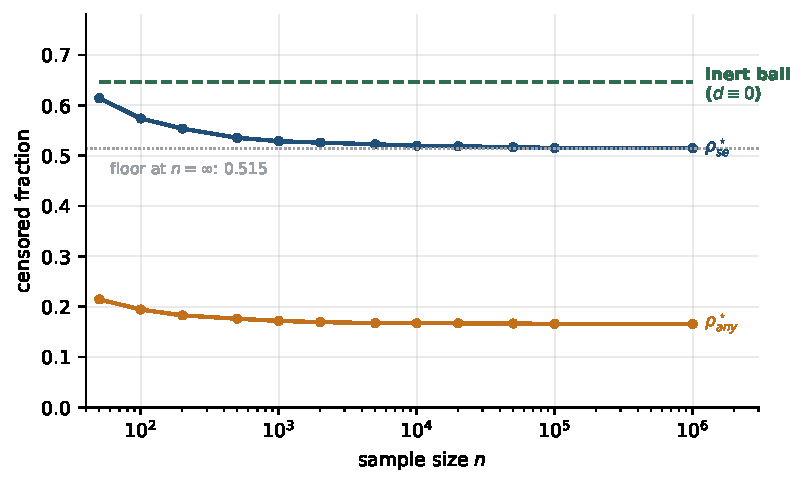
\includegraphics[width=0.68\textwidth]{aug_degeneracy.pdf}
\caption{Five orders of magnitude of sample size move the censoring of $\rhostar_{\mathrm{se}}$ by
ten points and then nothing. The dashed line is the share of problems whose one-reversal ball is
inert (64.6\,\%, identical at every $n$); the dotted floor, 0.515, is the share whose full ball
moves no estimate. The composite $\rhostar_{\mathrm{any}}$ is rarely censored, but 69\,\% of its
mass sits at one. Source: \texttt{e1prime/results/arm1\_analysis\_licensed\_K4.json}.}
\label{fig:aug-degeneracy}
\end{figure}

\begin{medido}[The censored bin, decomposed, same file, key \texttt{sweep}]
At $n = \infty$, of the 1,074 censored problems: none had every perturbation caught by Meek,
5.4\,\% had every perturbation lose amenability (a loud failure), and 94.6\,\% had consistent,
amenable members whose estimate did not move at all. At one reversal the displacement is exactly
zero for 64.6\,\% of problems, at $n = 200$ and $n = 20{,}000$ alike. The composite
$\rhostar_{\mathrm{any}}$ is censored for 0.166 of problems at $n = \infty$, with 69.1\,\% of the
mass at $\rhostar = 1$.
\end{medido}

Both statistics failed the pre-registered non-degeneracy profile, in opposite directions:
$\rhostar_{\mathrm{se}}$ is censored for half the problems and $\rhostar_{\mathrm{any}}$ puts two
thirds of them at one. The budget was the whole ball, so this is not budget censoring, and an exact
zero never exceeds a positive threshold, so it is not a sample-size effect. An inert ball is a
property of the problem: the reversed claims do not reach the part of the graph that $\Ostar$ reads.
Chapter~\ref{ch:locality} measures where those claims sit, and shows that much of the zero is a
published class-invariance fact rather than a finding. One label in the package is wrong here:
\texttt{REPORT.md} \S3 and \texttt{NUMBERS.md} call the series 0.554 to 0.515 the censoring of
$\rhostar_{\mathrm{any}}$. It is $\rhostar_{\mathrm{se}}$ (\texttt{SECONDARY\_rho\_se} in the JSON);
$\rhostar_{\mathrm{any}}$ goes from 0.183 to 0.166.

\prompt[conceito=censura-degenerescencia,dificuldade=0.75]{On the licensed ensemble the censoring
of $\rhostar_{\mathrm{se}}$ is 0.554 at $n = 200$ and 0.515 at $n = \infty$. What sets the floor,
and what does a censored problem almost always mean?}{At $n = \infty$ the standard error is zero,
so a problem is censored exactly when no consistent, amenable member of the full ball moves the
estimate at all; that share is 0.515 (gate G6). Of the 1,074 censored problems at $n = \infty$,
94.6\,\% are such exact zeros and 5.4\,\% lose amenability under every perturbation; none is
censored because Meek caught everything. Censored means the ball is inert, not that the analysis
is robust.}

\prompt[conceito=bola-inerte,dificuldade=0.7]{Why can no sample size remove the inert-ball mass?}%
{The instrument fires when $d(\rho) > z\,\mathrm{SE}_n$. $\mathrm{SE}_n$ shrinks like $n^{-1/2}$,
but an inert ball has $d(\rho) = 0$ exactly, and zero exceeds no threshold, not even the zero
threshold at $n = \infty$. The share of problems with $d(1) = 0$ is 64.6\,\% at every $n$ in the
grid.}

\begin{antes}
\antesq[vies-silencioso]{How many points of nominal 95\,\% coverage does one reversed claim cost,
among those Meek does not catch?}
\antesq[pre-registro]{Which width statistic did I pre-register for the robust interval, and why did
it flatter the method?}
\end{antes}

\section{ARM 2: what one wrong claim costs a confidence interval}

ARM 1 kept the knowledge true and asked how far the estimate could move. ARM 2 made it wrong. For
2,500 licensed SCMs, 20 datasets each and $n \in \{200, 1{,}000, 5{,}000, 20{,}000\}$, the analyst
receives $(C, \Kset_{\mathrm{asserted}}, \widehat\Sigma, n)$, where $\Kset_{\mathrm{asserted}}$
reverses $r \in \{0,1,2\}$ of the true claims. Reversals that Meek rejects are counted as caught
free and leave the sample. The analyst reports a naive interval $\hat\tau_0 \pm z\,\mathrm{SE}_n$
and a robust one, the hull of $\hat\tau_m \pm z\,\mathrm{SE}_m$ over consistent, amenable members
within $\rho$ reversals. $\tau$ decides coverage and does nothing else, and every SCM was rebuilt
from its seed with $\tau$ matching to $10^{-9}$ (0 failures in 2,500). This is the calibration
experiment that Section~4.3 of your rewrite of 30 August proposed.

\figref{fig:aug-coverage} carries the two numbers August could hand to a reviewer who does not work
with MPDAGs.

\begin{figure}[htbp]
\centering
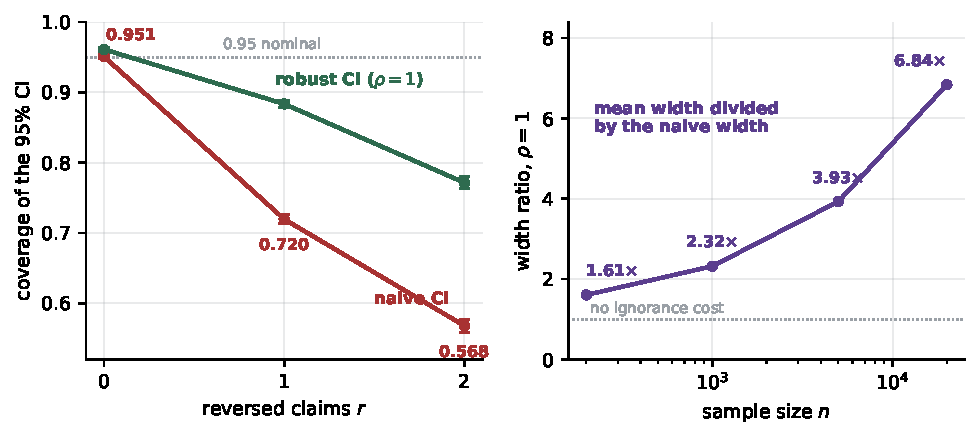
\includegraphics[width=0.94\textwidth]{aug_coverage.pdf}
\caption{Left: with the knowledge right the naive interval is calibrated; one accepted reversal
costs it 23 points and two cost 38, and ranging over single reversals recovers most of the first
loss. Right: that recovery gets more expensive as data grow, because the standard error shrinks
and the knowledge-induced spread does not. Source: \texttt{e1prime/results/arm2\_analysis.json}.}
\label{fig:aug-coverage}
\end{figure}

\begin{medido}[ARM 2, \texttt{rho\_breakdown/e1prime/results/arm2\_analysis.json}]
At $n = 20{,}000$ the naive interval covers 0.9509 [0.9481, 0.9533] with no reversal, 0.720 with
one and 0.568 with two; Meek rejects 23.6\,\% of single and 38.6\,\% of double reversals, and those
are excluded. At $r = 1$ the robust interval at $\rho = 1$ covers 0.8835, with width ratio to the
naive one of median 1.00, mean 6.84 and 90th percentile 23.3; its ball is inert for 69.3\,\% of
problems. At $\rho = 2$ it covers 0.9245 (mean ratio 11.6), the full ball 0.9306. When two claims
are wrong and the ball has radius one, coverage is 0.809 at $n = 200$ and 0.772 from $n = 5{,}000$
on. The mean width ratio at $r = \rho = 1$ is 1.61, 2.32, 3.93 and 6.84 across the four sample
sizes.
\end{medido}

The ignorance does not shrink with data: $\mathrm{SE}_n$ goes like $n^{-1/2}$ while $d(\rho)$ does
not depend on $n$. Even the full ball stops short of 0.95 (0.931 with one wrong claim, 0.912 with
two); the E1$'$ report attributes the residue to cells where the member that restores the truth is
itself not amenable and carries no estimate. Chapter~\ref{ch:gamma} prices a wrong claim again on
real structure.

\begin{armadilha}[The width statistic I pre-registered flattered the method]
The rule asked for coverage at least 0.90 at $r = \rho = 1$ and a \emph{median} width ratio below
$3\times$. Coverage was 0.8835 and the median 1.00: INCONCLUSIVE. The median is 1.00 by arithmetic,
since the ball is inert for 69\,\% of problems; the mean, $6.84\times$, would have failed the bar.
Both belong in the paper.
\end{armadilha}

\prompt[conceito=vies-silencioso,dificuldade=0.65]{Give the coverage of the naive 95\,\% interval
at $n = 20{,}000$ with 0, 1 and 2 reversed claims, and the exclusion that must travel with those
numbers.}{0.951, 0.720 and 0.568. They are computed among reversals Meek accepts: the check
catches 23.6\,\% of single and 38.6\,\% of double reversals, which leave the sample. The scope is
linear Gaussian iSCM, Erd\H{o}s--R\'enyi graphs with $p$ from 5 to 10, and the oracle CPDAG.}

\begin{antes}
\antesq[pre-registro]{Which August number was retired because the code that would have produced it
never existed?}
\antesq[banda-de-eficiencia]{Was the efficiency-only band, where $\Ostar$ moves and stays valid,
really empty?}
\end{antes}

\section{Corrections made before 31 August, and four since}

\texttt{rho\_breakdown/NUMBERS.md} closes with the corrections the package applied to itself.
Table~\ref{tab:pilot-corrections} gives them with the file that settles each, followed by the ones
found after it was written. The G1 row compresses two things in \texttt{NUMBERS.md} (``0.141 to
0.161''): the first cut divided by all single-reversal members and got 0.1085, and 0.141 is the
pilot's own value on its own grid.

\begin{table}[htbp]
\centering\footnotesize
\begin{tabular}{@{}>{\raggedright\arraybackslash}p{3.0cm}>{\raggedright\arraybackslash}p{2.1cm}>{\raggedright\arraybackslash}p{5.2cm}>{\raggedright\arraybackslash}p{4.0cm}@{}}
\toprule
what & first stated & as it stands & settled by \\
\midrule
silent bias at distance $\ge 1$ & 0 of 791 & retired: no distance function in the pilot code &
\texttt{locality/VERDICT.md} \\
gate G1, one reversal & 0.1085 & 0.161 on consistent members & \texttt{e1prime/RESULTS.md} \\
robust width ratio & median 1.00 & mean $6.84\times$ printed beside it & \texttt{arm2\_analysis.json} \\
gate G2 comparator & 0.336 & 0.271 (licensed grid); 0.284 measured, pass & \texttt{e1prime/RESULTS.md} \\
\midrule
series 0.554 to 0.515 & $\rhostar_{\mathrm{any}}$ & $\rhostar_{\mathrm{se}}$; $\rhostar_{\mathrm{any}}$
is 0.183 to 0.166 & \nolinkurl{e1prime/results/arm1_analysis_licensed_K4.json} \\
damage tail & up to $128\times$ & maximum $13.1\times$, median 0.591 ($n = 274$) &
\nolinkurl{pilot/results/linear_raw.json} \\
efficiency-only band & empty, 0 of 754 & empty for reversals only; 2.35--5.53\,\% under skeleton
deletions & \texttt{x3\_skeleton/RESULTS.md} \\
pilot budget & radius 8 & 6 moves in the pilot, 8 in E1$'$ & \texttt{pilot/code/run\_linear.py} \\
\bottomrule
\end{tabular}
\caption{Above the rule, the corrections \texttt{NUMBERS.md} lists; below it, those found later.
Paths are relative to \texttt{rho\_breakdown/}. Of the three things \texttt{NUMBERS.md} lists as never
run, two have run since: an estimated CPDAG (Chapters~\ref{ch:locality} and~\ref{ch:pest}) and
skeleton perturbation; nonlinear mechanisms beyond the pilot's 60 SCMs remain untested.}
\label{tab:pilot-corrections}
\end{table}

\begin{sonorio}[What August I licenses]
``In linear Gaussian SEMs on Erd\H{o}s--R\'enyi graphs with the true CPDAG, one reversed
background-knowledge claim that passes Meek's consistency check lowers the coverage of a nominal
95\,\% interval to 0.72 at $n = 20{,}000$. An interval that ranges over all single reversals
restores 0.88, at a mean width 6.8 times the naive one that grows with $n$.'' Not licensed:
``robust under an estimated CPDAG'', or $\rhostar$ as a well-behaved four-valued diagnostic.
\end{sonorio}

The two exercises rework the gate arithmetic and the censored bin from the files.

\begin{exercicio}[metodo=calculation,conceito=censura-degenerescencia]
(a)~The first cut of gate G1 divided silent-bias events by all single-reversal members and got
0.1085; Meek rejects 32.4\,\% of those members. Recover the rate on consistent members.
(b)~At $r = \rho = 1$ the mean width ratio is 3.93 at $n = 5{,}000$ and 6.84 at $n = 20{,}000$,
and the inert share stays near 69\,\%. Using only the dependence on $n$, predict the ratio at
$n = 2{,}000{,}000$.
(c)~A problem has $\rhostar_{\mathrm{se}} = 2$ in E1$'$. How many atomic moves of your
Section~4 is that?
\end{exercicio}
\begin{solucao}
(a)~The consistent members are $1 - 0.324 = 0.676$ of all, so $0.1085 / 0.676 = 0.1605$, the 0.161
recorded in the JSON (\texttt{G1\_silent\_bias\_rho1}); it sits inside the gate band 0.12--0.18.
(b)~The inert cells keep ratio 1 at every $n$, so it is the excess over one that scales. For the
other cells the knowledge spread is fixed and the naive width falls like $n^{-1/2}$, so the excess
grows like $\sqrt{n}$. Check: from 5,000 to 20,000 the excess goes from 2.93 to 5.84, a factor
1.99 against $\sqrt{4} = 2$. A further factor 100 in $n$ multiplies the excess by 10: about 58.4,
so a mean ratio near 59. This is an extrapolation of the functional form; the largest $n$ measured
is 20,000.
(c)~Two reversals, each a retraction and an assertion: four moves.
\end{solucao}

\begin{exercicio}[metodo=table-reading,conceito=bola-inerte]
The censored bin of $\rhostar_{\mathrm{se}}$ on the licensed ensemble (2,087 problems, $z = 1.96$),
read from \texttt{arm1\_analysis\_licensed\_K4.json}, in the table below.

\smallskip
\begin{center}\small
\begin{tabular}{@{}rcccc@{}}
\toprule
$n$ & censored problems & share loud & share robust & share with $d \equiv 0$ \\
\midrule
50 & 1,282 & 0.0452 & 0.9548 & 0.7925 \\
200 & 1,156 & 0.0502 & 0.9498 & 0.8789 \\
20,000 & 1,083 & 0.0536 & 0.9464 & 0.9381 \\
$\infty$ & 1,074 & 0.0540 & 0.9460 & 0.9460 \\
\bottomrule
\end{tabular}
\end{center}
Convert the shares into counts of three kinds of problem: loud, exactly inert, and robust with a
displacement that is not zero. Which of the three does the sample size act on, and on how many of
the 2,087 problems at most?
\end{exercicio}
\begin{solucao}
Multiplying out: loud problems are 58 at every $n$ ($1{,}282 \times 0.0452$, $1{,}156 \times
0.0502$, and so on). Exactly inert problems are 1,016 at every $n$. The remainder, robust with a
nonzero displacement smaller than $z\,\mathrm{SE}_n$, is 208 at $n = 50$, 82 at $n = 200$, 9 at
20,000 and 0 at $\infty$. Sample size acts only on that last group: at most 208 of
2,087 problems, and 82 from $n = 200$ on. At $n = \infty$ the censored problems are the 1,016 inert
ones and the 58 loud ones, 1,074 of 2,087 or 0.515: that is the floor. The shares in the last
column rise only because the denominator shrinks.
\end{solucao}

\naopasse[bola-inerte]{Say why, at $n = \infty$, a problem is censored exactly when no member of its
full ball moves the estimate, and why at $n = 200$ a censored problem can still have a moving
estimate. If you cannot, the step to redo is the definition of $\rhostar_{\mathrm{se}}$ with
$\mathrm{SE}_\infty = 0$.}

\section*{Chapter map}

\begin{center}
\begin{tikzpicture}[node distance=1.0cm and 1.2cm]
\node[cmapc] (pilot) {pilot, 17 July: reverse claims, re-close};
\node[cmapr, right=of pilot] (oracle) {$\rhostar$ compares with $\tau$: an oracle statistic};
\node[cmap, right=of oracle] (se) {E1$'$: yardstick $z\,\mathrm{SE}_n$, no $\tau$};
\node[cmap, below=of pilot] (unit) {one reversal = two atomic moves};
\node[cmapg, below=of oracle] (cost) {ARM 2: one wrong claim costs 23 points};
\node[cmapr, below=of se] (floor) {censoring floor 0.515: inert balls};
\node[cmapw, below=0.9cm of floor] (loc) {which claims are inert: Chapter~\ref{ch:locality}};
\draw[cedge] (pilot) -- node[above]{defines} (oracle);
\draw[cedge] (oracle) -- node[above]{repaired by} (se);
\draw[cedge] (pilot) -- node[left]{priced in} (unit);
\draw[cedge] (se) -- node[right]{stops at} (floor);
\draw[cedge] (se) -- node[above, sloped]{wrong claims} (cost);
\draw[cedge] (cost) -- (floor);
\draw[cedge] (floor) -- node[right]{explained in} (loc);
\end{tikzpicture}
\end{center}

\chapter{August II: locality, the firewall, and a wrong skeleton}
\label{ch:locality}

One intuition ran through August: a wrong claim far from the query rarely matters. This chapter
follows it through five runs and says what is left. Some of it is a result, some is a lemma that
Henckel, Perkovi\'c and Maathuis had already published, and some is dead, including two sentences I
sent you on 31 August. Table~\ref{tab:loc-status} is the ledger; the sections give the evidence.
Throughout, \emph{distance} means skeleton distance from a claim's edge to $\{X,Y\}$, the minimum
over both endpoints. The files call it \texttt{hop}; it is not the covering hop of
Chapter~\ref{ch:vocabulary}.

\begin{table}[htbp]
\centering\footnotesize
\begin{tabular}{@{}>{\raggedright\arraybackslash}p{7.0cm}>{\raggedright\arraybackslash}p{7.6cm}@{}}
\toprule
August claim & status on 16 September \\
\midrule
censoring of $\rhostar_{\mathrm{any}}$ separates by distance & result, per ensemble: $26.7\times$,
$13.4\times$, $59.7\times$, $3.0\times$ \\
``$\Ostar$ is a local functional; 0 of 791 at distance $\ge 1$'' & dead: 142 of 3,639 and 70 of
10,615; 791 has no provenance \\
one reversal off $X$ and $Y$ never moves $\Ostar$ & true by enumeration at $p \le 5$; 95.8\,\% of
it is class invariance \\
knowledge beyond one hop need not be elicited & dead: identification changes at distance 2 \\
C-FIREWALL & conjecture, complete census at $p \le 5$ \\
firewall with an estimated $\Chat$ & result: degrades monotonically with discovery quality \\
false identification gains & result: not bounded by distance \\
locality survives a wrong skeleton (X3) & INCONCLUSIVE; the two-hop cut is post hoc \\
the efficiency-only band is empty & corrected: 2.35--5.53\,\% under skeleton deletions \\
only retractions can break a fixed valid $Z$ & lemma, by refinement \\
\bottomrule
\end{tabular}
\caption{Where each August claim about locality stands. ``Dead'' means refuted by our own
measurements, not merely unproven. Each row's files are named in the section that discusses it.}
\label{tab:loc-status}
\end{table}

\begin{antes}
\antesq[o-star-otimo]{Before any locality run, what had the 14 August experiments already said about
$\Ostar$-relevance?}
\antesq[k-background-knowledge]{Do Guo and Perkovi\'c ever perturb the background knowledge they
enumerate within?}
\end{antes}

\section{Prehistory: the three re-rank experiments of 14 August}

Three small runs on 14 August shaped what came after. None of them is in the paper, and one of them
is a literature read rather than a measurement.

\textbf{E2}, R1-closed finiteness (\texttt{rerank\_2026-08-14/e2-r1-finiteness/RESULTS.md}). Your
draft's tiered corruption model is close to its T-move arm. When the error is a variable moved
between tiers, R1-only closure equals full Meek closure in every member (39,267 of 39,267), which
Bang and Didelez entail. When the
error is a reversed claim, it holds in 0.8416 of members, so flip errors break the premise of the
lemma. Containment is real but only in the tail: the 90th percentile of orientations changed per changed
claim is 1 for tier moves against 2 for flips. The same run found that the form of the knowledge buys nothing (tiered
against generic under flips, $p = 0.49$); the error model does.

\textbf{E3}, $\Ostar$-relevance (\texttt{e3-ostar-relevance/RESULTS.md}). A metric weighting wrong
claims by their role in $\mathrm{pa}(\mathrm{cn})\setminus\mathrm{forb}$ beat edit distance at predicting silent bias, AUC
0.842 against 0.637. Against a plain count of wrong claims touching $X$ or $Y$ the gain fell to
$+0.029$, under the pre-declared bar of 0.05, and the specifically $\Ostar$ tier was anti-predictive
(AUC 0.409). The content was locality, not adjustment-set membership.

\textbf{E4}, a full read of Guo and Perkovi\'c (arXiv:\allowbreak{}2010.08611) and Taeb, Guo and Henckel
(arXiv:\allowbreak{}2511.10625v3) (\texttt{e4-guo-perkovic-read/\allowbreak{}RESULTS.md}). Guo and Perkovi\'c take $\Kset$ as
true throughout (``perturb'', ``wrong'' and ``misspecif'' occur zero times); Taeb et al.'s
Section~6 perturbs the graph with the knowledge fixed. Two narrowings bind the paper: the separation
of identification from estimation is Guo and Perkovi\'c's sentence, and their Corollary~8 already
gives one adjustment set per member.

\begin{antes}
\antesq[lei-de-localidade]{The E1$'$ locality table was said to separate by 13 to 27 times. What do
its four rows actually give?}
\antesq[localidade]{Which two measurements killed the sentence ``$\Ostar$ is a local functional of
the graph''?}
\end{antes}

\section{Locality, measured and then cut down to size}

\begin{ideia}[The intuition]
$\Ostar = \mathrm{pa}(\mathrm{cn}(X,Y)) \setminus \mathrm{forb}(X,Y)$ reads the causal paths from $X$ to $Y$ and one layer
of parents around them. A claim that never reaches that region cannot move it, so an inert ball
should mean claims far from the query.
\end{ideia}

\figref{fig:aug-locality} is the E1$'$ measurement. Each licensed problem is placed by the smallest
distance of any of its claims, and the censoring of $\rhostar_{\mathrm{any}}$ at $n = 20{,}000$ is
low when some claim touches the query and near one when none does.

\begin{figure}[htbp]
\centering
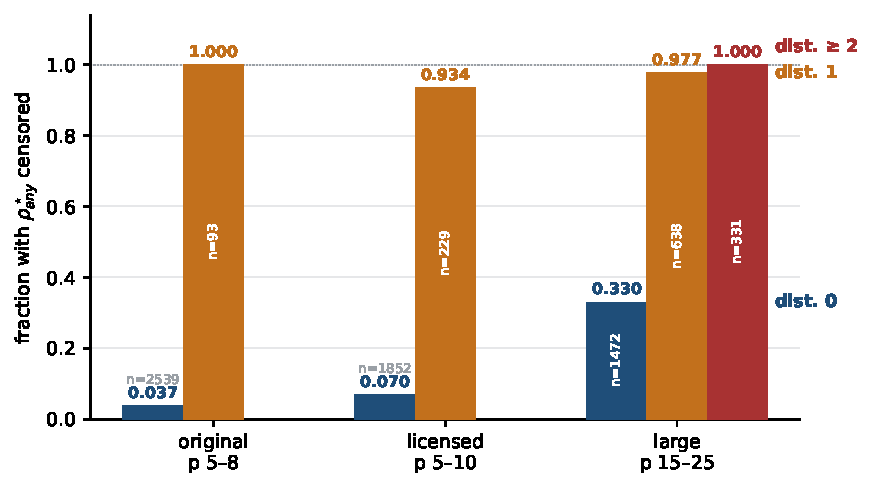
\includegraphics[width=0.72\textwidth]{aug_locality.pdf}
\caption{The distance of the nearest claim governs whether the radius has anything to say, but the
size of the gap depends on the ensemble: $26.7\times$, $13.4\times$ and $3.0\times$ for the three
shown. Licensed at distance~1 is 0.9345 in the JSON (\texttt{NUMBERS.md} rounds to 0.935). Of the
331 \texttt{large} SCMs in the red bar, 57 have every claim in a component disconnected from the
query. Source: \texttt{e1prime/results/arm1\_analysis\_*\_K4.json}.}
\label{fig:aug-locality}
\end{figure}

\begin{armadilha}[Four defects in the table I sent you]
The separation ratios are 26.7, 13.4, 59.7 (\texttt{k8}, $n = 22$ at distance~1) and 3.0
(\texttt{large}), so ``13 to 27 times'' holds for two rows of four. The weakest cell,
\texttt{k8}/K4 at 0.778 ($n = 27$), was left out. ``Invariant in $n$ to four decimals'' is true at
distance~1 (0.9345 at $n = 2{,}000$, $20{,}000$ and $\infty$); at distance~0 the licensed value
moves from 0.0724 to 0.0697 to 0.0680. And $\rhostar_{\mathrm{any}}$ folds in loud failures: of the
38 uncensored SCMs whose claims all sit at distance $\ge 1$, 37 lose amenability, 1 has a genuine
change at two reversals, and none moves the estimate at one (\texttt{locality/x2/RESULTS.md} \S3).
\end{armadilha}

Two runs of 19 August then attacked the sentence ``$\Ostar$ is a local functional, and no
misstatement at distance at least 1 moved it (0 of 791)''. The number went first: the pilot code
contains no distance function at all, so 791 could not have been computed
(\texttt{locality/VERDICT.md} \S4). X1 (\texttt{locality/x1/}) built the operator for spurious
required edges on non-adjacent pairs, replacing one true claim with a spurious one under the semantics of
b-LOAD, our CIKM paper's noise operator. On the \texttt{original} ensemble such a replacement at distance $\ge 1$ moved
$\Ostar$ into invalidity 142 times in 3,639; pooled over three ensembles, 13 in 2,919 at distance
$\ge 2$ and 0 in 931 at distance $\ge 3$. X2 enumerated instead of sampling. At
$p \le 5$, over every CPDAG, every reachable MPDAG, every query and both orientations of every
undirected edge, a single reversal off $X$ and $Y$ never changed $\Ostar$: 0 of 136,200 far trials,
against 184,332 of 307,584 near ones. Joint reversals did: 70 of 10,615 knowledge sets from the
E1$'$ archive whose every misstatement lies at distance $\ge 1$ changed $\Ostar$, all 70 into
invalidity, each with a misstatement at distance exactly 1, the smallest at $p = 5$. The same
enumeration records 360 identification changes at distance~2, which ended ``knowledge beyond one hop
need not be elicited''.

\begin{medido}[What the far zero is made of, \texttt{locality/x2/code/run\_lemma.py}]
At $p = 5$ the far zero rests on 137,040 trials in which both orientations of the claim leave the
query amenable (\texttt{lemma\_p5.json}, disconnected components included). In 131,280 of them, 95.8\,\%, the base MPDAG is
already amenable. The informative trials, where the claim decides something, number 5,760, all at
distance~1; at distance~2 there are none. The split by base is from my notes of 23 August, which
recount the strata with the same code.
\end{medido}

When the base is amenable, $\Ostar$ is constant over the whole class, so no refinement of it can
move $\Ostar$ at any distance, near ones included. I traced this class invariance to Henckel,
Perkovi\'c and Maathuis (JRSS-B 84(2), 2022, Lemma~E.7 in their appendix); I have not re-read that
lemma in the published text, so check the number before citing it. The consequence is plain: most
of the far zero is a published fact, the pilot's ``wrong knowledge was harmless in 75 of 75
CPDAG-amenable SCMs'' is the same fact, and what distance adds is an incidence condition (the claim
does not touch $X$), not a decay law.

\begin{noprato}[In your draft]
The paragraph ``Over-claiming does not pay'' in your Section~6 (``once a valid set is identified,
adding more truthful claims does not improve statistical efficiency'') is this class invariance.
Cite it rather than argue it.
\end{noprato}

\prompt[conceito=localidade,dificuldade=0.75]{Which two measurements killed ``$\Ostar$ is a local
functional of the graph'', and what survives in its place?}{X1: a spurious required edge replacing
a true claim at distance $\ge 1$ moved $\Ostar$ into invalidity 142 times in 3,639
(\texttt{original}). X2: 70 of 10,615 knowledge sets whose every reversed claim lies at distance
$\ge 1$ changed $\Ostar$, all into invalidity. What survives is narrower: a single reversed claim
that does not touch $X$ or $Y$ never changed $\Ostar$ in the complete enumeration at $p \le 5$, and
95.8\,\% of those trials had an amenable base, where class invariance already forbids any change.}

\prompt[conceito=distancia-em-saltos,dificuldade=0.7]{Why is ``distance $\ge 1$'' in the X2 zero
better read as an incidence condition, and what is the informative denominator at $p = 5$?}%
{Distance $\ge 1$ holds exactly when the claim's edge touches neither $X$ nor $Y$, and no graded
distance does any work: the informative trials all sit at distance~1 and there are none at
distance~2. Of 137,040 far trials with both orientations amenable, 131,280 have an amenable base,
where $\Ostar$ cannot move at any distance; 5,760 carry information.}

\begin{antes}
\antesq[consistencia-de-k]{For a query already identified by adjustment, can a spurious edge that
passes the coherence check make the reported $\Ostar$ invalid?}
\antesq[vies-silencioso]{How does the protection change when the CPDAG is estimated by PC?}
\end{antes}

\section{The firewall: what the consistency check buys}

\begin{ideia}[Checked is not true, but it is not nothing]
Meek's check never decides truth. For a query that adjustment already identifies, though, a false
adjacency claim that passes the check appears never to invalidate the set the analyst reports: the
check acts as a firewall for validity, and only there. The surprise is that the graph after the claim has a
skeleton no member of the true class has, yet the set read from it is valid in the truth.
\end{ideia}

Stated for a single spurious claim, it reads as follows.

\begin{formulabox}[C-FIREWALL, a conjecture]
Let $\Gz$ be an MPDAG amenable for $(X,Y)$, $\{a,b\}$ non-adjacent in its skeleton, and $H$ the Meek
closure of $\Gz$ plus $a \to b$. If $H$ has no directed cycle, then either $H$ is not amenable (a
visible refusal) or $\Ostar(X,Y,H)$ is a valid adjustment set in every DAG of $[\Gz]$.
\end{formulabox}

The evidence for it is a census, not a proof.

\begin{medido}[The census, \texttt{locality/x2/cfirewall/results/SUMMARY.json}]
0 violations in 70,375,325 trials and 103,105,398 (trial, DAG) checks. The census is complete at
$p = 3, 4, 5$ for one claim (and for two claims at $p = 4, 5$, three at $p = 4$); $p = 6, 7, 8$ are
samples, with a rule-of-three bound below $4.3 \times 10^{-8}$. The detector has power: when the
check fails and the edge is stamped anyway, 3,005,488 of 13,791,476 reported sets (21.8\,\%) are
invalid. Pointwise over 791,484 evaluations at $p \le 5$, the conflict test never fires and
``has a directed cycle'' coincides with ``not extendable'', so the whole hypothesis is acyclicity
(\texttt{checks\_agree.txt}).
\end{medido}

It is a conjecture, not a theorem. The first proof handle offered (adding the edge only grows
$\mathrm{cn}$) is false; what holds in every enumerated trial is $\Ostar(H) \cap \mathrm{forb}(\Gz) = \emptyset$, which settles the first clause of the adjustment
criterion for the whole class, given a further hypothesis that held in every census trial; the second clause is closed by a sufficient condition in 98.0\,\% of
checks and open in the rest. X1 looked like a contradiction (1.1\,\% silent bias, 64 of 5,815, among
coherent spurious claims). My reading is that the operators differ: X1 replaces a true claim, so each
of its perturbations is a retraction plus an assertion, closed claim by claim, while the census adds
one spurious edge on top of the full closed $\Gz$.

\begin{medido}[With PC instead of the oracle, \texttt{locality/x2/chat/RESULTS.md}]
PC written from scratch; with oracle tests it returns the true CPDAG in 150 of 150 gate draws. 400
SCMs per cell, $p$ from 6 to 10, $\alpha = 0.01$. Among reports valid before the claim whose $\Ostar$
moved, a checked spurious claim leaves them invalid in 10.9\,\% at $n = 200$, falling to 2.4\,\% at
$n = 50{,}000$ and to 0 of 22,282 with oracle tests; stamped past a failed check, 17.4 to 34.8\,\%.
Discovery error alone leaves 35.9\,\% of base reports invalid at $n = 200$, 17.1\,\% at $n = 50{,}000$.
\end{medido}

My first version of that table compared rates on different conditioning sets and reversed the sign
of the conclusion; the numbers above condition on a valid base report. Two further arms were written
and run on 23 August itself, in the same working session, so they corroborate nothing independently.
The false-gain search (\texttt{falsegain/results/search\_6\_7\_8\_23.json}) adjudicated every report
transition against the truth on random DAGs with $p$ from 6 to 8: no report that was already
identified became unsound under a checked claim, but when a checked claim turned a refusal into an
estimate, the estimate was wrong in 13,988 of 17,936 cases for a false orientation (78.0\,\%) and in
24,895 of 49,467 for a spurious edge (50.3\,\%). Exercise~\ref{ex:loc-chain} builds the family that
takes this to any distance. The refutation arm (\texttt{refutation/conjectureA/exh6\_result.json})
enumerated all 1,067,825 CPDAGs on six nodes, 149,123,280 orientation additions on amenable bases, and found $\Ostar$
unchanged in every one; that is class invariance again, and it killed nothing.

\prompt[conceito=consistencia-de-k,dificuldade=0.75]{State C-FIREWALL and the two numbers that make
its zero meaningful.}{For an MPDAG $\Gz$ amenable for $(X,Y)$ and a spurious claim $a \to b$ on a
non-adjacent pair, if the closure $H$ is acyclic then either $H$ is not amenable or $\Ostar(H)$ is
valid in every DAG of $[\Gz]$. The census found 0 violations in 70,375,325 trials, complete at
$p \le 5$; and the control arm, where the check fails and the edge is stamped anyway, has 21.8\,\%
invalid sets, so the detector can fire.}

\begin{antes}
\antesq[vies-silencioso]{If the discovery method misses one edge, does the damage fall off with the
distance of that edge from the query?}
\antesq[testemunha]{In the worked example, how many claims have to be retracted before the reported
set stops being valid, and when does the estimate first move?}
\end{antes}

\section{X3: a wrong skeleton, and one problem end to end}

For the 3 September meeting you asked what happens when the discovery output itself is wrong. X3 answered for
one kind of error: $\Chat$ is the CPDAG of the true DAG with one edge deleted, which models a missed
weak edge rather than what a CI test actually returns. The run covers 9,721 SCMs and all 130,120
single-edge deletions, with population $\Sigma$. The claims of $\Kset$ are kept where their edge is
still undirected. A smoke test found the true CPDAG not amenable for the query in 18 of 19 draws,
so before any outcome was computed the arm with knowledge became the primary one.

\begin{figure}[htbp]
\centering
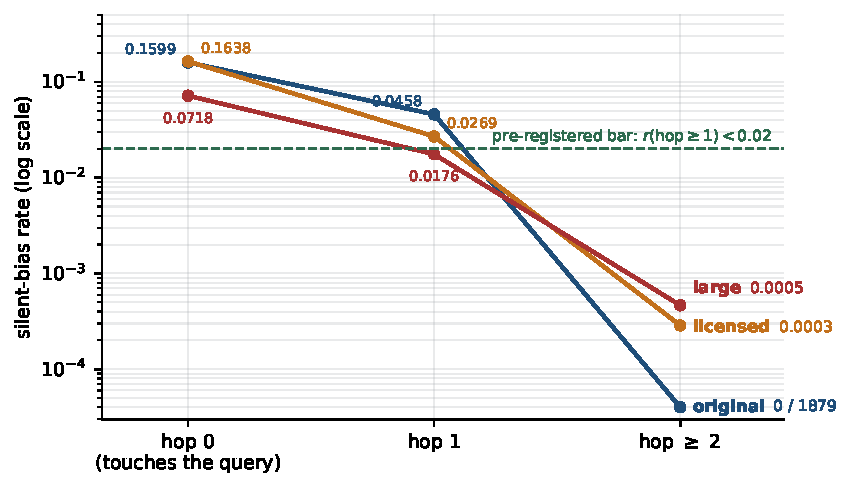
\includegraphics[width=0.7\textwidth]{x3_hops.pdf}
\caption{A missed edge at distance~1 still breaks the set in 2.7\,\% of amenable cases on the
licensed ensemble; pooled with distance $\ge 2$ that is 2.3\,\%, above the pre-registered 0.02,
so the rule returns INCONCLUSIVE. The cut at two
hops looks clean but was chosen after seeing these lines. The \texttt{original} zero (0 of 1,879)
is drawn at the axis floor. Source: \texttt{x3\_skeleton/results/x3\_analysis.json}.}
\label{fig:x3-hops}
\end{figure}

\figref{fig:x3-hops} carries the verdict. The rule asked for a ratio of at least 5 between the
silent-bias rate at distance~0 and at distance $\ge 1$, and a rate below 0.02 at distance $\ge 1$.
The ratio is 7.10; the rate is 0.0231. Pooled over the three ensembles, distance~0 gives 5,066 of
36,829 (0.1376) and distance $\ge 2$ gives 15 of 35,501 (0.000423), a 326-fold drop, but that cut is
post hoc and has to be re-registered and re-run before it goes near the paper. The sentence the
paper can print today is that the pre-registered test was inconclusive and the data suggest a
threshold at two edges rather than one; and ``a distant skeleton error rarely does damage'', never
``does little damage''.

\figref{fig:x3-taxonomy} holds what does not depend on the verdict. Without any knowledge the CPDAG
answers the query by adjustment in 8.2, 16.9 and 55.8\,\% of problems, so on most of them there is
nothing to be robust about until knowledge arrives. The efficiency-only band exists: $\Ostar$ moves
and stays valid in 2.35, 2.65 and 5.53\,\% of deletions. The median absolute weight of the deleted
edge is the same for damaging and harmless deletions (0.5726 against 0.5583 on licensed, inverted on
\texttt{large}), so strength does not predict damage and distance does. Severity does not fall with
distance: among silent-bias events on licensed at distance $\ge 1$ the relative bias has median
0.39, 90th percentile 1.75 and maximum 1,204.

\begin{figure}[htbp]
\centering
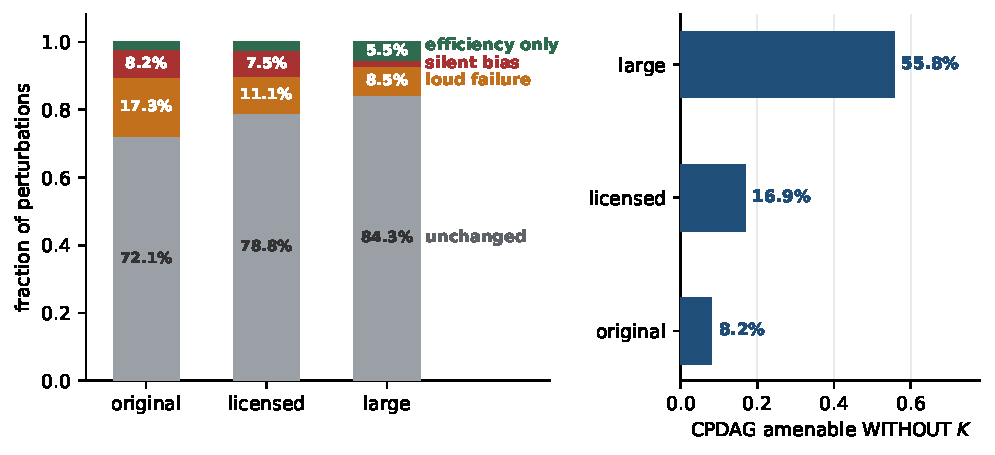
\includegraphics[width=0.85\textwidth]{x3_taxonomy.pdf}
\caption{Left: the efficiency-only band (green) is not empty under skeleton deletions, which
corrects the 0 of 754 we measured with claim reversals. Right: without knowledge the question of
robustness rarely arises, because the CPDAG seldom identifies the effect. Source:
\texttt{x3\_skeleton/results/x3\_analysis.json}.}
\label{fig:x3-taxonomy}
\end{figure}

The worked example (\texttt{x3\_skeleton/results/worked\_example.txt}, seed 4906, $p = 7$) was built
for the 3 September meeting. The names are attached by topological position and claim nothing
empirical. The query is the effect of \textsf{Statin} on \textsf{CardiacEvent}; the analyst asserts
\textsf{Exercise}~$\to$~\textsf{BMI} and \textsf{BMI}~$\to$~\textsf{BloodPressure}, Meek propagates
\textsf{BloodPressure}~$\to$~\textsf{Statin}, and $\Ostar = \{\textsf{BMI}, \textsf{Exercise}\}$
gives $-0.4191$, which is also the true effect. A move is adding or retracting one claim and closing
again (\texttt{worked\_example.py}, function \texttt{neighbours}).

\begin{figure}[htbp]
\centering
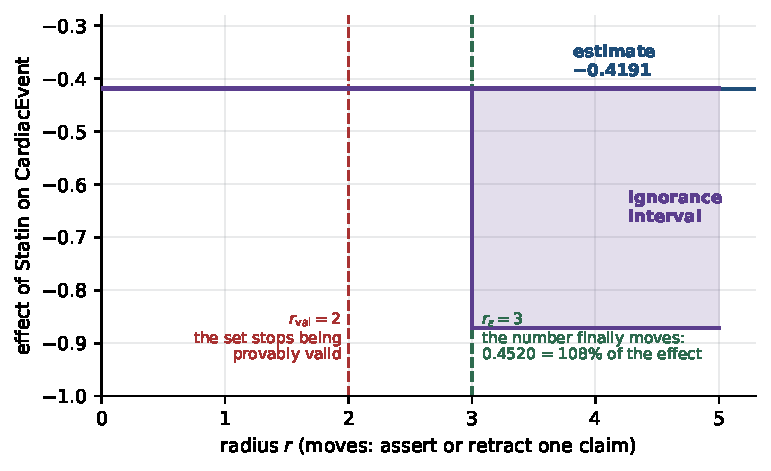
\includegraphics[width=0.64\textwidth]{aug_worked_example.pdf}
\caption{The set stops being provably valid after two retracted claims, but the estimate does not
move until radius three, where the interval opens by 0.4520, 108\,\% of the effect. One radius would
have raised the alarm one step early. The axis counts claim additions and retractions. Source:
\texttt{worked\_example.txt}.}
\label{fig:aug-example}
\end{figure}

\figref{fig:aug-example} is the case that justifies reporting validity and estimate separately:
fragile identification, stable estimate. The witness reads ``the estimate holds unless
\textsf{BMI}~$\to$~\textsf{BloodPressure} is retracted and \textsf{Exercise}~$\to$~\textsf{BMI} is
retracted''. Building it also produced a lemma. If $G'$ refines $G$ then $[G'] \subseteq [G]$, so a
$Z$ valid in every DAG of $[G]$ stays valid in every DAG of $[G']$: asserting a consistent claim can
never break a fixed valid set, only retracting can. It is the same monotonicity that
Chapter~\ref{ch:table4} audits on the ledger.

\prompt[conceito=vies-silencioso,dificuldade=0.7]{What did X3 return under its pre-registered rule,
and why is the two-hop cut not a result?}{INCONCLUSIVE. The ratio of silent-bias rates, distance~0
against distance $\ge 1$, is 7.10 and passes the bar of 5, but the rate at distance $\ge 1$ is
0.0231 and fails the bar of 0.02. The cut at two hops (0.1376 against 0.000423, 326 times) was chosen
after seeing the data, so it is a hypothesis to re-register and re-run on fresh draws.}

\prompt[conceito=testemunha,dificuldade=0.7]{In the worked example, what does ``fragile
identification, stable estimate'' mean in numbers?}{The fixed set $\{\textsf{BMI},
\textsf{Exercise}\}$ stops being valid in every DAG of the graph after two claim retractions
($\rval = 2$), while the interval of estimates is the single point $-0.4191$ up to radius two and
opens to $[-0.8711, -0.4191]$ only at radius three, a width of 0.4520, or 108\,\% of the effect.}

\begin{exercicio}[metodo=counterexample,conceito=localidade]
\label{ex:loc-chain}
Refute with a construction: ``a false claim that passes Meek's check and lies two or more edges from
the query can at worst make the analyst refuse to report.'' Use a path of five nodes.
\end{exercicio}
\begin{solucao}
Take the skeleton $c_0 - c_1 - c_2 - X - Y$ and the true DAG $Y \to X \to c_2 \to c_1 \to c_0$, so
the true effect of $X$ on $Y$ is $\tau = 0$. A directed path has no v-structure, so the CPDAG is
fully undirected; the path $X - Y$ starts undirected and the query is not amenable: the analyst
refuses. Now assert the false claim $c_0 \to c_1$, at distance 2 from $\{X,Y\}$. It is consistent,
and R1 propagates it along the path:
\begin{center}
\begin{tikzpicture}[x=1.5cm, font=\scriptsize\sffamily]
\foreach \i/\n in {0/c_0,1/c_1,2/c_2,3/X,4/Y} {\node[nodo] (n\i) at (\i,0) {$\n$};}
\draw[falsa] (n0) -- (n1);
\draw[propagada] (n1) -- (n2); \draw[propagada] (n2) -- (n3); \draw[propagada] (n3) -- (n4);
\node[rotulo, anchor=north] at (0.5,-0.3) {asserted, false};
\node[rotulo, anchor=north] at (2.5,-0.3) {propagated by R1};
\end{tikzpicture}
\end{center}
Now the query is amenable, $\Ostar = \mathrm{pa}(Y) \setminus \mathrm{forb} = \emptyset$, and the
analyst reports the regression of $Y$ on $X$, which is not zero because $Y$ causes $X$. The same
construction works at distance $k$ on $k + 3$ nodes; \texttt{locality/x2/falsegain/results/chain\_k0\_k8.log}
checks $k = 0, \dots, 8$ (all unsound, absolute bias 0.85 to 0.95 against $\tau = 0$). The
firewall does not apply: the base was not identified.
\end{solucao}

\begin{exercicio}[metodo=drawing,conceito=testemunha]
Draw $\Gz$ of the worked example, marking asserted, propagated, compelled and undirected edges. Then
retract each claim alone and say what the closure returns and whether $Z = \{\textsf{BMI},
\textsf{Exercise}\}$ stays valid. Why is $\rval = 2$?
\end{exercicio}
\begin{solucao}
\begin{center}
\begin{tikzpicture}[x=1.55cm, y=0.8cm, font=\scriptsize\sffamily]
\node[nodot] (age) at (0,1) {Age};
\node[nodot] (smk) at (1.2,1) {Smoking};
\node[nodot] (ex) at (2.5,1) {Exercise};
\node[nodot] (bmi) at (2.5,0) {BMI};
\node[nodot] (bp) at (4.0,0) {BloodPressure};
\node[nodot] (st) at (5.5,0) {Statin};
\node[nodot] (ce) at (4.0,-1.1) {CardiacEvent};
\draw[livre] (age) -- (smk); \draw[livre] (smk) -- (ex);
\draw[afirmada] (ex) -- (bmi); \draw[afirmada] (bmi) -- (bp);
\draw[propagada] (bp) -- (st);
\draw[aresta] (bmi) -- (ce); \draw[aresta] (ex) to[out=-10,in=100] (ce); \draw[aresta] (st) -- (ce);
\end{tikzpicture}
\end{center}
Thick blue: the claims; dashed: propagated; grey arrows: compelled; plain lines: undirected.
Retracting \textsf{BMI}~$\to$~\textsf{BloodPressure} alone returns the same graph: R1 re-derives it
from \textsf{Exercise}~$\to$~\textsf{BMI}, since \textsf{Exercise} and \textsf{BloodPressure} are
not adjacent. Retracting \textsf{Exercise}~$\to$~\textsf{BMI} alone leaves that edge undirected, but
\textsf{Statin} keeps no undirected edge, so the query stays amenable and $Z$ valid. Retracting both
returns the CPDAG: \textsf{Statin}~$-$~\textsf{BloodPressure} is undirected, the query is not
amenable, and some DAG of the class has \textsf{Statin}~$\to$~\textsf{BloodPressure}~$\to$~\textsf{BMI}
with \textsf{BMI} a mediator. So $\rclaim = 2$, and the witness's first step moves nothing, a step a covering-hop count would not
charge. The hop walk is not cheaper for that: it pays three steps here, one of them for the propagated
orientation between \textsf{BloodPressure} and \textsf{Statin} ($\rhop = 3$, Chapter~\ref{ch:vocabulary};
the unit comparison is Chapter~\ref{ch:table4}). I checked the three closures
with \texttt{x3\_skeleton/code/}.
\end{solucao}

\naopasse[localidade]{Name the difference in operator that lets X1 find silent bias from coherent
spurious claims while the firewall census finds none. If you cannot, the step to redo is what X1 does
to the claim its spurious edge replaces.}

\section*{Chapter map}

\begin{center}
\begin{tikzpicture}[node distance=0.9cm and 1.1cm]
\node[cmapc] (loc) {E1$'$: censoring separates by claim distance};
\node[cmapr, right=of loc] (dead) {``$\Ostar$ is local'', 0/791: dead};
\node[cmap, right=of dead] (inv) {class invariance: most of the far zero};
\node[cmapg, below=of loc] (fw) {C-FIREWALL: census, 0 in 70\,M};
\node[cmap, below=of dead] (chat) {PC instead of oracle: firewall degrades};
\node[cmapr, below=of inv] (gain) {false gains: no distance protects};
\node[cmapw, below=of chat] (x3) {X3, wrong skeleton: INCONCLUSIVE, band exists};
\draw[cedge] (loc) -- node[above]{over-read as} (dead);
\draw[cedge] (dead) -- node[above]{replaced by} (inv);
\draw[cedge] (loc) -- node[left]{identified queries} (fw);
\draw[cedge] (fw) -- node[above]{estimated $\Chat$} (chat);
\draw[cedge] (inv) -- node[right]{unidentified base} (gain);
\draw[cedge] (chat) -- node[right]{wrong skeleton} (x3);
\draw[cedge] (gain) -- node[above, sloped]{the other side of} (fw);
\end{tikzpicture}
\end{center}


\part{Early September: what the radius should measure}
\chapter{Early September: what should the radius measure?}
\label{ch:redefinition}

This chapter covers 3 to 9 September: the week in which I tried to repair the degeneracy of $\rval$, ended
up changing the question the radius answers, and then found that one contrast I had drawn, between my random
draws and your corpus, came from how the two pipelines admitted queries rather than from structure. The mass at
one retraction itself is real: it returns on the frozen frame in Chapters~\ref{ch:where} to~\ref{ch:tables}.
Unit: the validity radius of my harness and of your corpus is a breadth-first distance in covering hops, so I
write it $\rhop$ here; the null radius counts retracted claims. The files of that week are in \texttt{rho\_breakdown/radius\_redef\_2026-09-07/}
unless a path says otherwise.

\begin{antes}
\antesq[rval]{Your deck of 3 September closed the WP0 fork. Which branch did it support, and which did it
reject?}
\antesq[censura-degenerescencia]{If a statistic puts almost all of its mass on two values, can a quantile or a
mean of it repair that?}
\end{antes}

\section{After 3 September: the defect I set out to repair}

Your deck worked exactly on one eight-variable clinical graph, all 48 MPDAGs enumerated, and closed the WP0
fork in its own words. The diagnostic-tool branch was supported ($\rval = 3,
3, 2$, no saturation at 1). The trade-off paper was not, because all 14 valid adjustment sets share $\rval = 3$
and the efficiency--robustness frontier is flat. A week later your Phase~2 on
\texttt{experiments/survival-and-pareto} falsified the Pareto premise twice and abandoned it under its
pre-registered trigger: truthful knowledge that identifies a set always identifies the same one, so precision
never moves, and what knowledge buys is identifiability (385 of 1,431 proposals, 26.9\,\%, justified no valid
set). Nothing in this document disputes either conclusion.

In the same days I had the opposite picture on small random problems. On 7 September I re-measured the validity radius, in covering hops ($\rhop$),
with an independent harness: random DAGs on six nodes, one to six undirected CPDAG edges, up to three true
claims, every query with an identified optimal set kept, the whole space enumerated around $\Gz$.

\begin{medido}[$\rhop$ on 400 random problems, \texttt{harness.py}]
$\rhop = 1$ on 190 (47.5\,\%), 2 or 3 on 9 (2.3\,\%), unreached on 201 (50.2\,\%): 97.7\,\% of the mass on
$\{1,\infty\}$ (\texttt{EXPERIMENTS.md}, \S1).
\end{medido}

I read this as worse than a bias toward 1. A biased statistic can be recentred; a nearly binary one answers a
single question (does some single retraction break the set?), and any quantile or mean of it inherits the two
values. That reading drove the week. Section~\ref{sec:redef-harness} shows which part of it described my harness.

\begin{antes}
\antesq[retracao]{Retracting a claim and reversing it look like two ways of doubting it. Are they two objects?}
\antesq[casco]{If the hedge is restricted to the claims that matter, does the interval get narrower?}
\end{antes}

\section{Thirty-seven candidates, two lemmas, one object}
\label{sec:redef-object}

The target was a definition that is not degenerate, keeps a soundness statement, and gives a narrow interval
where no damage is present. I wrote down 37 candidate redefinitions and audited each against measurements
before refining any (\texttt{plan.json}). Nineteen were killed, most because on almost every problem they
returned $\rval$, $\rval - 1$ or a contradiction-count radius that moves with them; all seven quantile or mass
radii and all six weighted minima died that way. The arithmetic is short: first shells held at most 7 elements,
so any quantile above $0.857$ returned the minimum (160 of 160 problems), and for a well-posed centre the broken
share one hop out never exceeded one half (maximum $0.5000$ over 840 problems). The survivors had replaced the
minimum by a range of effects. The object they share is easiest to see on a five-node example
(\figref{fig:redef-hull}).

\begin{exemplo}[Three claims, three behaviours]
True DAG $C\to X$, $C\to Y$, $C\to W$, $X\to M$, $M\to Y$; query $(X,Y)$; true effect $1.2623 \times 0.7518 =
0.949$. The CPDAG keeps $C\to Y\leftarrow M$ and leaves $C-W$, $C-X$, $M-X$ undirected; its four extensions give
the effects $\{-0.203, 0.746, 0.949\}$, whose hull $[-0.203, 0.949]$ (width $1.152$) is the \emph{blanket}. The
analyst asserts $\Kset = \{C\to W, C\to X, X\to M\}$ and reports the point $0.949$. Retracting $C\to X$ opens the
hull to $[0.746, 0.949]$; retracting $C\to W$ changes the graph but not the effect; retracting $X\to M$ changes
nothing, since R1 forces it back from $C\to X$. The union over single retractions is $[0.746, 0.949]$, $0.176$ of
the blanket. Asserting $X\to C$ instead would give the point $0.746$, off the truth.
\end{exemplo}

\begin{figure}[H]
\centering
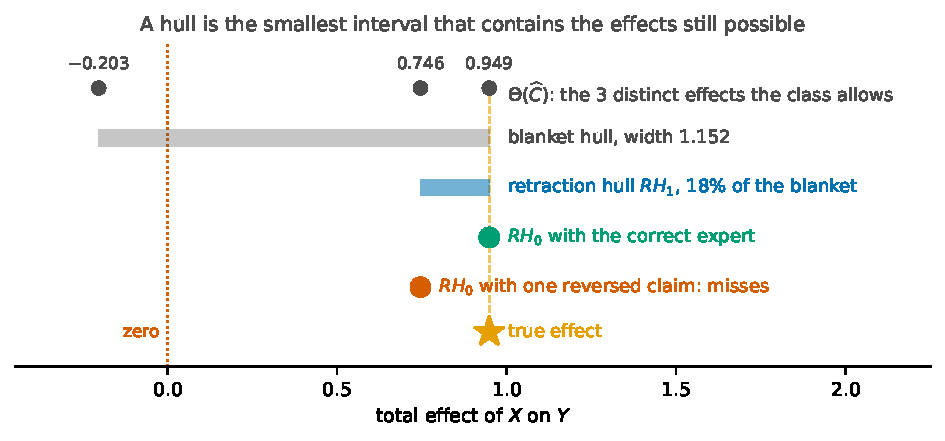
\includegraphics[width=0.84\linewidth]{redef_hull_example.pdf}
\caption{With the claims right the report is a point on the truth and one retraction widens it to under a fifth
of the blanket; with one claim reversed the report misses, and nothing at budget zero can show it.}
\label{fig:redef-hull}
\end{figure}

\begin{definicao}[Retraction hull]
With $\Theta(G)$ the set of effects of $X$ on $Y$ over the DAG extensions of $G$ (adjusting for the parents of $X$
in each), $\mathrm{RH}_j = \operatorname{hull} \bigcup_{|S| \le j} \Theta(\mathrm{Meek}(\Chat, \Kset \setminus
S))$. $\mathrm{RH}_0$ is the report and $\mathrm{RH}_{|\Kset|}$ the blanket. If $\Chat$ is the true class and at
most $j$ claims are false, $\mathrm{RH}_j$ contains the true effect, with no continuity assumption. Later chapters
call it the knowledge interval $\Ir{j}$.
\end{definicao}

Two lemmas turned most of the surviving candidates into this one object.

\begin{lema}[L1 and L2]
\textbf{L1, retraction equals reversal.} For every budget $b$, retracting at most $b$ claims reaches exactly the worlds
reached by reversing at most $b$ claims: a world compatible with $\mathrm{Meek}(\Chat, \Kset\setminus S)$ contradicts
$\Kset$ on exactly one $\sigma \subseteq S$. \textbf{L2, screens are width-neutral.} If $\Theta(\Gz)$ is a point and
$Z_0 = \Ostar(\Gz)$ is valid, a claim whose retraction leaves $Z_0$ valid leaves $\Theta$ unchanged; the hull over the
load-bearing claims equals the hull over all of $\Kset$.
\end{lema}

Both were checked numerically before anything was built on them.

\begin{medido}[Lemmas and frontier, \texttt{EXPERIMENTS.md}]
L1: 0 differences over 573 problems. L2: 250 of 250 and 300 of 300. Frontier (\texttt{confirm.py}: seven nodes, up to four
claims, 300 problems per arm): the first budget reaching 95\,\% coverage costs $0.710$ of the blanket's width with one
reversed claim and $0.903$ with two, and at one reversed claim the one-retraction hull \emph{is} the blanket on
67.2\,\% of problems (\S\S2--3).
\end{medido}

L1 makes ``flip up to $b$ claims'' and ``retract up to $b$ claims'' one object: reversal models the error,
retraction hedges it. L2 takes my fourth proposed direction, identifying which claims are false, out of any width
table. Locality measured in coverage on 8 September is the same fact in another currency: at a matched budget of
one retraction, retracting only claims that touch the query covers 0.998 at 0.621 of the blanket's width against 1.000
at 0.630 for any claim, with 3.13 instead of 4.31 enumerations (\texttt{local\_hedge.py}). It pays in computation and in what to ask the expert, not in width.

\begin{armadilha}[Coverage 1.000 in every cell]
The first run of \texttt{confirm.py} covered at every budget, budget zero included: the claims were drawn
truthfully, so there was nothing to be robust to. Asking what could have made the number differ from 1 caught it;
the fix reverses some claims and keeps only draws that survive Meek closure, the errors the consistency check misses.
\end{armadilha}

An audit of the frontier also asked what the width is made of. On informative problems with one reversed claim the class disputes
whether $X$ causes $Y$ at all in 86.9\,\%; among the worlds that agree on direction the width is $0.314$ of the
blanket, and exactly zero in 60.7\,\% (\texttt{EXPERIMENTS.md}, \S4). About two thirds of the hedged width is a
dispute about causal order. Only 20 to 24\,\% of drawn problems were informative at all.

\prompt[conceito=retracao,dificuldade=0.7]{State L1 and give the one-line reason it holds. What does it
merge?}{For every budget $b$, the union of retractions of at most $b$ claims equals the union of reversals of at most
$b$ claims. A world compatible with the re-closed graph after retracting $S$ contradicts $\Kset$ on exactly one subset
$\sigma \subseteq S$, so the retraction of $S$ is the disjoint union of the reversals of its subsets. It merges the
``flip claims'' and ``retract claims'' families: reversal models the error, retraction builds the hedge.}

\prompt[conceito=casco,dificuldade=0.75]{A colleague proposes to rank which claims are false and hedge only those, to
get a narrower interval. What does L2 say, and in which currency can the idea still pay?}{L2: the hull over the
load-bearing claims already equals the hull over all claims, so no screen narrows the interval. The idea pays in cost
(the query-local screen needs 3.13 instead of 4.31 enumerations per problem, for a width of 0.621 against 0.630 of the blanket) and in
elicitation (claims away from the query moved coverage by 0.2 points, so do not ask about them).}

\prompt[conceito=casco,dificuldade=0.8]{With one reversed claim the mean width ratio of the one-retraction hull is 0.710,
and the hull equals the blanket on 67.2\,\% of problems. What is the mean ratio on the rest?}{From $0.672 \times 1 +
0.328\,\bar x = 0.710$, $\bar x \approx 0.116$. Where the selective hull does anything it costs about an eighth of the
blanket; the average saving of 29\,\% is carried by a third of the problems, and a headline must say so.}

\begin{antes}
\antesq[nulidade]{Rosenbaum's $\Gamma$ does not ask whether the identifying assumption holds. What does it ask?}
\antesq[estrato]{If four problems in five leave no doubt about the effect, what does a robustness statistic measure on
them?}
\end{antes}

\section{The null radius: Rosenbaum's question, taken literally}
\label{sec:redef-null}

\begin{ideia}[What $\Gamma$ asks]
Not whether there is unmeasured confounding, but how strong it would have to be before the conclusion falls. For
background knowledge: how many of my claims would have to fall before I can no longer claim an effect?
\end{ideia}

On 8 September I wrote that down with the machinery above. Two things change with respect to the harness radius:
the unit ($\rhop$ walks covering hops, the new radius counts retracted claims) and, more importantly, the predicate
that stops the search ($\rhop$ stops where some graph invalidates $Z$, the new radius where the hull reaches zero). The audit of 7 September had rejected
a hop-ball ancestor, unreached on 183 of 200 draws; this one is read off the claim-indexed hull.

\begin{definicao}[Null radius]
$\rnul = \min\{ j : 0 \in \mathrm{RH}_j \}$, and $\rnul = \infty$ if no budget puts zero in the hull. Every effect
compatible with any retraction of at most $\rnul - 1$ claims has the same sign.
\end{definicao}

Its first measurement looked like a failure: over all drawn problems with a non-zero effect, $\rnul$ was ``never'' on
84\,\% (\texttt{signradius.py}). The population was the problem. Most drawn problems have a blanket of width zero, where
nothing can move; conditioning on the \emph{informative} stratum, the problems with positive blanket width, swaps the
two statistics (\figref{fig:redef-stratum}).

\begin{medido}[The informative stratum, \texttt{stratum.py}]
\begin{tabular}{@{}lrr@{}}
1,800 problems, one reversed claim & all & informative (381, 21.2\,\%) \\ \midrule
$\rhop = 1$ & 43.9\,\% & 89.5\,\% \\
effective values $2^H$ of $\rhop$ (hops) / of $\rnul$ (claims) & 2.28 / 2.66 & 1.51 / 3.46 \\
\end{tabular}
\end{medido}

\begin{figure}[H]
\centering
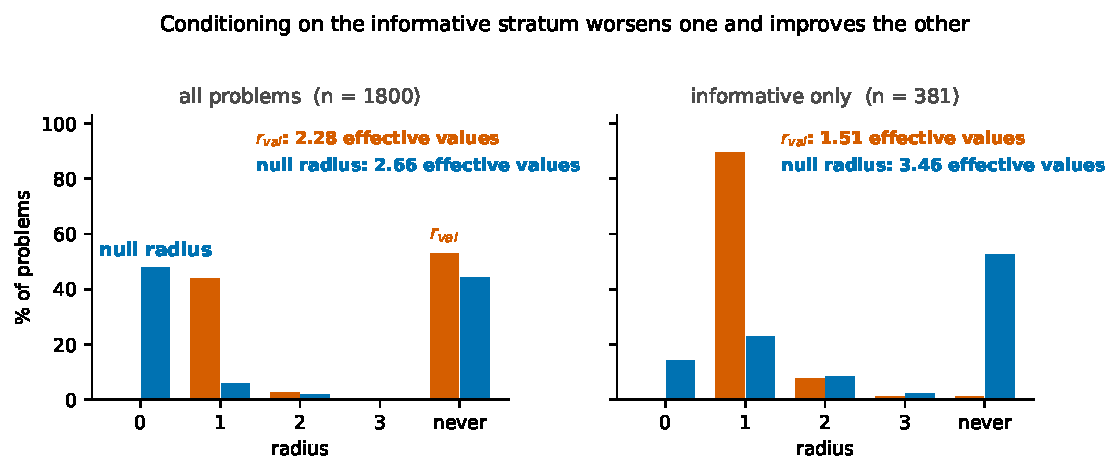
\includegraphics[width=0.86\linewidth]{redef_stratum.pdf}
\caption{Where the class leaves any doubt about the effect, the validity radius ($\rhop$) is almost a constant and the null radius spreads
over four levels.}
\label{fig:redef-stratum}
\end{figure}

The stratum is defined by the blanket, which reads neither $\Kset$ nor the planted errors, so this is not selection on
the outcome. But $1.51$ against $3.46$ is conditional on a selection and does not show that the redefinition improved
the statistic. Your
\texttt{LOG.md} of session~6 retracts a coverage conclusion for the same reason (543, 182, 106 admissible rows: a
composition effect).

\begin{sonorio}[The null radius, as it can be printed]
Under the stated equivalence class, every effect compatible with retracting any $\rnul - 1$ of the analyst's
orientation claims has the same sign; some set of $\rnul$ claims, once retracted, admits a zero or opposite-sign effect.
\end{sonorio}

\prompt[conceito=nulidade,dificuldade=0.65]{The harness's validity radius and $\rnul$ differ in two ways. Name both,
and say which one changes what the number means.}{The unit: the harness radius ($\rhop$) is a breadth-first distance in
covering hops, $\rnul$ counts retracted claims. And the stopping predicate, which is the one that changes the meaning:
$\rhop$ stops when some graph makes the committed set $Z$ invalid, a property of an intermediate step; $\rnul$ stops when
the hull of possible effects contains zero, a property of the conclusion. A set can become invalid while every compatible
effect stays far from zero, and then the validity radius raises an alarm about nothing the analyst asserted to the world.}

\begin{antes}
\antesq[dois-paineis]{On your real networks at full coverage, is $\rhop = 1$ more or less frequent than on my random
problems?}
\antesq[banda-plugin]{Computed from $\widehat\Sigma$, in which direction does a point-hull null radius err?}
\end{antes}

\section{9 September: the ``never'' contrast was an admission rule}
\label{sec:redef-harness}

On 9 September I recounted your \texttt{results/axisa3/instances.jsonl} instead of copying the session~6 report, matching
knowledge coverage at 1.0.

\begin{medido}[Two populations, \texttt{stratum.py} against \texttt{results/axisa3/instances.jsonl}]
\begin{tabular}{@{}lrrrrr@{}}
 & $\rhop = 1$ & on $\{1,\infty\}$ & never & largest & eff.\ values \\ \midrule
my random draws (1,800) & 43.9\,\% & 96.8\,\% & 52.9\,\% & 4 & 2.28 \\
39 real networks (543 rows) & 69.8\,\% & 69.8\,\% & 0.0\,\% & 14 & 2.61 \\
\end{tabular}
\end{medido}

Neither 52.9\,\% nor 0\,\% ``never'' describes structure; each describes an admission rule. The mass at one retraction
is a different matter and does not go away: on the frozen frame of 11--13 September $\rclaim = 1$ on all 540
full-coverage rows (Chapter~\ref{ch:where}), $\rnul$ is nearly binary (Chapter~\ref{ch:gamma}), and one retraction
returns the whole-class interval on all 26 informative queries of T3's 37 eligible (Chapter~\ref{ch:tables}). Your \texttt{THEOREMS.md} §14 already
says the saturation at 1 is not a definitional artefact.

\begin{armadilha}[Two comparisons of mine, both across populations]
I had first noted that $\rhop = 1$ falls from about 80\,\% to 61.1\,\% on real structure; the 61.1\,\% pools three
coverage levels, and at coverage 1.0 it is 69.8\,\%. The table repeats the error at a deeper level. My draws kept every
query whose claims survive Meek closure, including queries with no causal path, and \texttt{stratum.py} counted a query
with no identified set as ``never''. Your \texttt{fast\_gate} rejects such queries and, at full coverage, admits a pair
only if one retraction breaks $\Ostar$, so ``never'' is impossible by construction, as your \texttt{LOG.md} notes. Your
random arm, gated the same way, has 0 unreached radii in 2,334 draws (\texttt{results/axisa2/random\_analysis.txt}).
\end{armadilha}

Within your corpus, $\rhop = 1$ on 69.8\,\% of full-coverage rows, with a tail up to 14 that Chapter~\ref{ch:where} explains. Every width, coverage and direction number of Section~\ref{sec:redef-object} remains a measurement on my small random problems.

The same day I computed $\rnul$ from $\widehat\Sigma$ on your four Gaussian networks, whose coefficients are fitted to real
data. The routine reads no DAG, but its inputs were the oracle CPDAG and claims from \texttt{select\_knowledge}, read from the
truth (Chapter~\ref{ch:where}): the run tests the estimator, not a deployment. \texttt{arth150} hit the 20-minute wall at coverage 0.5 and is left out.

\begin{medido}[$\rnul$ from $\widehat\Sigma$, \texttt{rho\_breakdown/rnull\_real\_2026-09-09/direcao\_fast.py}]
Coverage 1.0, 145 queries: oracle $\rnul = 1$ on 49 (34\,\%), $\infty$ on 96; the zero is structural (some extension has an
effect of exactly zero) on 40 of the 49. Share of replicates whose estimate exceeds the oracle, claiming robustness that is
not there:

\smallskip
\begin{tabular}{@{}lrrrr@{}}
$n$ & 200 & 1,000 & 5,000 & 20,000 \\ \midrule
point hull & 24.7\,\% & 22.3\,\% & 20.6\,\% & 18.1\,\% \\
95\,\% band & 1.5\,\% & 0.1\,\% & 1.7\,\% & 1.0\,\% \\
\end{tabular}
\end{medido}

\prompt[conceito=dois-paineis,dificuldade=0.8]{Why do the 52.9\,\% ``never'' of my draws and the 0\,\% of your corpus not show
that random graphs make the radius degenerate?}{They come from different admission rules. My draws admitted every Meek-consistent
query, including queries with no causal path, and counted unidentified queries as ``never''. Your gate rejects those and, at full
coverage, admits a pair only if one retraction breaks $\Ostar$, which makes an unreached radius impossible; your gated random arm
has 0 unreached in 2,334. The contrast is between pipelines, not structures.}

\naopasse[dois-paineis]{Write down the single condition in \texttt{fast\_gate} that makes an unreached radius impossible at full
coverage. If you cannot, reread the red box above: Chapter~\ref{ch:where} builds on it.}

\begin{exercicio}[metodo=diagnosis,conceito=banda-plugin]
A draft sentence reads: ``On \texttt{ecoli70}, from $n = 20{,}000$ samples, the null radius of the query is infinite, so the
conclusion that $X$ affects $Y$ survives the retraction of every claim.'' The radius was computed with the point hull.
Diagnose the sentence and rewrite it.
\end{exercicio}
\begin{solucao}
The estimator: the point hull overstates the null radius on 18.1\,\% of replicates even at $n = 20{,}000$, because a
structural zero becomes $\pm\varepsilon$ in $\widehat\Sigma$ and lands on either side; recompute with the 95\,\% band (at most
1.7\,\%). The scope: the run used the oracle CPDAG and knowledge read from the truth, so nothing follows about errors in the class.
The reading: $\rnul = \infty$ says no budget puts zero in the hull, not that the effect is large. Rewrite: ``Under the stated equivalence class, and with the 95\,\% band from
$\widehat\Sigma$, no retraction of the analyst's orientation claims admits a zero or opposite-sign effect of $X$ on $Y$.''
\end{solucao}

\begin{exercicio}[metodo=calculation,conceito=nulidade]
Five-node example. (a) $\mathrm{RH}_1$ and its share of the blanket. (b) $\rnul$, given $\mathrm{RH}_2$ is the blanket. (c)
$\rnul$ with $X\to C$ asserted (report $0.746$, $\mathrm{RH}_1$ the blanket), and did the report cover the truth? (d) With the right
claims $\rhop = 1$; compare with (b).
\end{exercicio}
\begin{solucao}
(a) The retractions give $\{0.949\}$, $[0.746, 0.949]$, $\{0.949\}$, so $\mathrm{RH}_1 = [0.746, 0.949]$, width $0.203$, and
$0.203/1.152 = 0.176$. (b) $\mathrm{RH}_0$ and $\mathrm{RH}_1$ exclude zero and $\mathrm{RH}_2 = [-0.203, 0.949]$ contains it:
$\rnul = 2$. (c) $\{0.746\}$ misses $0.949$; $\mathrm{RH}_1$ contains zero, so $\rnul = 1$, and the same single retraction
restores coverage. (d) Validity of $Z$ breaks one hop away while the sign of the effect survives any single retraction: $\rhop
= 1$ raises an alarm that $\rnul = 2$ does not share.
\end{solucao}

\section*{Chapter map}
\begin{center}
\begin{tikzpicture}[x=1cm, y=1cm]
\node[cmapr, text width=3.1cm] (rv) at (0,0) {$\rhop$ nearly binary on my harness};
\node[cmap, text width=3.1cm] (c37) at (4.3,0) {37 candidates, 19 killed};
\node[cmapc, text width=3.1cm] (rh) at (8.6,0) {retraction hull $\mathrm{RH}_j$};
\node[cmapr, text width=3.1cm] (adm) at (0,-1.45) {the ``never'' contrast: an admission rule};
\node[cmap, text width=3.1cm] (st) at (4.3,-1.45) {informative stratum};
\node[cmapc, text width=3.1cm] (r0) at (8.6,-1.45) {null radius $\rnul$};
\node[cmapg, text width=3.1cm] (band) at (12.9,-1.45) {95\,\% band, not the point hull};
\draw[cedge] (rv) -- node[above, align=center]{motivates} (c37);
\draw[cedge] (c37) -- node[above, align=center]{L1, L2\\ merge} (rh);
\draw[cedge] (rh) -- node[right]{stop at $0 \in \mathrm{RH}_j$} (r0);
\draw[cedge] (st) -- node[above, align=center]{where it\\ varies} (r0);
\draw[cedge] (r0) -- node[above, align=center]{from\\ $\widehat\Sigma$} (band);
\draw[cedge] (rv) -- node[right]{traced 9 to 11 Sep} (adm);
\end{tikzpicture}
\end{center}

\chapter{Where to evaluate, and three defects in the old corpus}
\label{ch:where}

On 10 September I stopped to ask where the radius should be evaluated at all, since every result so far rested on
sampled graphs that do not look like a deployment. Answering it meant reading the committed pipeline end to end, and
the reading found three defects in the corpus of \texttt{results/axisa3/}. Two of my own first diagnoses were wrong,
and both corrections are below. The notes and scripts of these two days are in
\texttt{rho\_breakdown/eval\_protocol\_2026-09-11/}; the protocol they produced is the one executed in
Chapters~\ref{ch:frame} to~\ref{ch:pest}.

\begin{antes}
\antesq[invariante]{An evaluation instance has five coordinates. Which of them does a list of datasets fix?}
\antesq[invariante]{In which two places may the true DAG appear without breaking a deployment claim?}
\end{antes}

\section{What a deployed instance is}

\begin{ideia}[Not a list of datasets]
An evaluation methodology is a sampling distribution over instances $I = (G_{\mathrm{true}}, \Chat, (X,Y), \Kset, D_n)$.
Swapping Erdős--Rényi graphs for real networks fixes one coordinate; if $\Kset$ is still read from the true DAG, the ball
stays centred on the truth, over better graphs.
\end{ideia}

What a deployed analyst holds fixes the rule for every coordinate.

\begin{formulabox}[The invariant]
$r = r(\Chat, \Kset, X, Y, \widehat\Sigma, n)$: a functional of analyst-observable quantities only. The true DAG enters
twice, both times after the deployment rows are frozen: to generate the sample, as nature does, and to audit whether the
promise held. A row is in the audit arm when the hash of its CPDAG source equals the hash of its generating DAG, decided
by comparing bytes rather than reading a label.
\end{formulabox}

With the invariant written down, the comparison that motivated the question reads differently. Section~6.2 of your draft
contrasts separation of at least 2 in 45.4\,\% of real instances with 14.2\,\% of synthetic ones. Both numbers are in your
files, over different denominators.

\begin{medido}[Separation $\ge 2$, \texttt{results/axisa3/instances.jsonl}]
Real: 210 rows, 45.4\,\% of the 463 with defined separation, 25.3\,\% of all 831 admissible. Random arm (\texttt{results/axisa2/random\_control.jsonl}): 14.2\,\% of 1,587
measurable draws pooled over five generators; Erdős--Rényi alone 12.5\,\%, and 3.6\,\%, 14.7\,\%, 24.1\,\% in its dense,
medium and sparse cells. Undefined separation: 44.3\,\% of real rows, 17.1\,\% of random ones.
\end{medido}

The sparse cell, 24.1\,\%, sits next to the real corpus over its full denominator, 25.3\,\%; density drives most of the gap,
and the real corpus (mean degree 1.60 to 9.86, median 2.92, \texttt{results/axisa3/descriptive\_structure.csv}) was never
matched to a density cell. The reason to evaluate on real structure is the invariant, not a degeneracy of random graphs.

\prompt[conceito=invariante,dificuldade=0.7]{Where may the true DAG appear without breaking a deployment claim, and what
makes those two places harmless?}{It may generate the sample, which is what nature does and all the analyst receives, and it
may audit the certificate after the deployment rows are frozen and hashed. What makes them harmless is the order: both come
after the freeze, so no reported observable quantity can have been chosen by looking at the truth.}

\begin{antes}
\antesq[oraculo-k]{At coverage 1.0, what is $\Gz$ in the committed corpus?}
\antesq[amenabilidade]{518 queries are rejected at partial coverage as \texttt{o\_g0\_not\_identified}. Did the optimal-set
criterion kill them?}
\end{antes}

\section{Defect 1: the analyst's knowledge is read from the true DAG}

In \texttt{src/bkrobust/benchmarks/measure.py}, \texttt{select\_knowledge(dag, cpdag, coverage)} takes the true DAG and calls
\texttt{knowledge\_to\_recover} (\texttt{src/bkrobust/demo/example.py}), which repeatedly asserts the true orientation whose
Meek closure orients the most edges; it sorts the result and keeps an evenly spaced fraction. Every claim is true, and at full
coverage the closure is the true DAG.

\begin{armadilha}[Correction 1: a default read as a measurement]
I first wrote that $\Gz$ had no undirected edge in all 831 admissible rows, reading \texttt{g0\_undirected\_edges = 0}. The
field is assigned only in the intractable-extensions branch (line 240 of \texttt{measure.py}) and keeps the dataclass default
elsewhere. Rebuilt row by row: the 543 rows at coverage 1.0 are fully oriented, hence equal to the true DAG, and all 288
partial-coverage rows keep an undirected edge. The same silent default sits in \texttt{k\_g0} on rejected rows.
\end{armadilha}

The rejection \texttt{o\_g0\_not\_identified} fires 286 times at coverage 0.25, 232 at 0.5, never at 1.0. The four-node
\texttt{mediator} network shows the mechanism.

\begin{exemplo}[\texttt{mediator}, query $X \to I$]
The DAG $Z\to X$, $Z\to I$, $X\to I$, $X\to Y$, $I\to Y$ has no v-structure, so the CPDAG is fully undirected. The sorted
recovering set is $(X\to I,\ Z\to I,\ Z\to X)$. At coverage 1.0, $\Gz$ is the DAG, $\Ostar = \{Z\}$, admitted. At 0.5,
$\operatorname{round}(3 \times 0.5) = 2$ and the stride keeps the first two claims; $X - Z$ stays open, one extension makes $Z$ a
confounder ($\Ostar = \{Z\}$) and the other a mediator ($\Ostar = \varnothing$), and the row is rejected.
\end{exemplo}

\begin{center}
\begin{tikzpicture}[x=1cm,y=0.9cm]
\foreach \dx/\lab/\zx/\zi/\xi in {0/{true DAG}/aresta/aresta/aresta, 4.3/{coverage 1.0: admitted}/afirmada/afirmada/afirmada,
  8.6/{coverage 0.5: $X - Z$ open, rejected}/livre/afirmada/afirmada} {
\begin{scope}[xshift=\dx cm]
\node[nodo] (Z) at (0.9,1.0) {$Z$}; \node[nodo] (X) at (0,0) {$X$};
\node[nodo] (I) at (1.8,0) {$I$}; \node[nodo] (Y) at (0.9,-1.0) {$Y$};
\draw[style=\zx] (Z) -- (X); \draw[style=\zi] (Z) -- (I); \draw[style=\xi] (X) -- (I);
\ifdim\dx pt=0pt \draw[aresta] (X) -- (Y); \draw[aresta] (I) -- (Y);
\else \draw[propagada] (X) -- (Y); \draw[propagada] (I) -- (Y); \fi
\node[font=\scriptsize\sffamily] at (0.9,-1.6) {\lab};
\end{scope}}
\end{tikzpicture}
\end{center}

\begin{armadilha}[Correction 2: Lever 0 recovers nothing]
I first read this example as the optimal-set definition deleting the realistic case, since it enumerates extensions and gives
up when they disagree, and proposed Lever 0: the closed form $\Ostar = \mathrm{pa}(\mathrm{cn}(X,Y)) \setminus
\mathrm{forb}(X,Y)$ would bring the rows back. It does not. All 518 rejected rows are non-amenable; here $X - Z \to I$ is a
possibly causal path starting with an undirected edge. The deletion is right and the label is wrong. Caught by running
\texttt{is\_amenable} and the closed form on every rejected row before writing the fix.
\end{armadilha}

The numbers behind both halves of that correction:

\begin{medido}[The diagnosis, \texttt{diagnostico\_amenabilidade.py}]
518 of 518 rejections non-amenable, 0 recoverable. Over every same-size subset of the recovering set on the eight smallest
networks (1,238 subsets), 29 of 40 non-degenerate rejected cases have another subset of that size that keeps the query
amenable, 11 have none, and 61 more are degenerate ($\operatorname{round}(1 \times 0.5) = 0$ leaves no knowledge). The 12
September differential agrees: the closed form returns a set where enumeration said ``not identified'' on 0 rows
(\texttt{results/stage0/lever0\_differential.json}).
\end{medido}

So the defect is the \texttt{sorted()} in the thinning, not the optimal criterion: where it can be tested, the query usually
dies because the analyst holds the wrong claims, chosen by alphabetical order. The stride is not even nested ($\Kset(0.25)
\not\subseteq \Kset(0.5)$ on \texttt{diabetes}, \texttt{ecoli70}, \texttt{magic-irri}, \texttt{munin1}), so a coverage sweep is not
a retraction sequence. The 518 are not missing data either: their radius is already zero, and Stage~0 added an identifiability radius (retractions until
adjustment stops identifying the effect) that is defined exactly where the current radius dies.

\begin{noprato}[What landed on 12 September, and what no patch fixes]
Additive patches to \texttt{measure.py}, committed behaviour as default: a \texttt{nested} selection (prefix of one seeded
permutation); \texttt{not\_amenable} split from \texttt{o\_g0\_not\_identified}; a three-valued verdict for $\Ostar$; both silent
fields assigned on every branch; the dispatch leg as a column. On 213 recomputed committed rows no admissible row moved
(\texttt{experiments/stage0\_differential.py}). A better stride fixes the size of $\Kset$, never its origin; that takes knowledge
that does not come from the truth (Chapter~\ref{ch:frame}).
\end{noprato}

\prompt[conceito=lever0,dificuldade=0.75]{What did Lever 0 recover of the 518 rejected rows, and what is the actual defect?}{Nothing:
all 518 are non-amenable, so no definition of the optimal set can certify them; the deletion is right and the label
\texttt{o\_g0\_not\_identified} is wrong. The defect is the thinning in \texttt{select\_knowledge}, which sorts the recovering set
alphabetically and keeps an even stride; on 29 of 40 testable cases another subset of the same size would have kept the query
amenable.}

\begin{antes}
\antesq[unidade-afirmacao]{The gate admits a pair only if something happens under one retraction. What, and what does that fix?}
\antesq[regra-livre]{How often does a hop count from $X$ to the adjustment set, computable from $\Chat$ and $\Kset$, reproduce the
committed radius?}
\end{antes}

\section{Defects 2 and 3: what the committed radii count}

\texttt{fast\_gate} in \texttt{measure.py} reads the true DAG five times: whether $Y$ descends from $X$, the optimal set on the DAG,
the validity of that set and of the empty set, and a loop that admits a pair only if retracting a single claim of the recovering
set, with Meek re-closure, makes the optimal set invalid. At coverage 1.0 the asserted set is the recovering set, so admission is
the definition of $\rclaim = 1$.

\begin{medido}[The claim unit at full coverage, \texttt{stage0/rclaim\_cov1.py}]
540 rows (\texttt{pathfinder} excluded): $\rclaim = 1$ on all 540. Committed hop radius 1 on 377, 2 on 102, 3 on 43, 4 to 14 on
18. Median asserted claims 5, median closure $|K_{\Gz}|$ 12. The share of single retractions that break the set, $\phi_1$, runs
from 0.034 to 1, median 0.30.
\end{medido}

Section~6.3 of your draft names the sharpest case. In \texttt{paths} (17 nodes), hop radius 14, the analyst asserts one claim, $15\to 14$, at
the top of the fifteen-node chain component, and R1 orients the thirteen other chain edges from it. Retract it and the chain un-orients at once:
the hop count is the length of a Meek cascade and the tolerable number of wrong claims is zero. The paragraph commented out in your
\texttt{06\_simulation.tex}, saying $\rclaim = 1$ on all 540 rows by construction, is correct and should go back in.

\begin{center}
\begin{tikzpicture}[x=1.05cm,y=1cm]
\foreach \n/\x in {15/0,14/1,13/2,12/3} \node[nodo] (n\n) at (\x,0) {\n};
\node at (4,0) {$\cdots$};
\foreach \n/\x in {3/5,2/6,1/7} \node[nodo] (n\n) at (\x,0) {\n};
\node[nodo] (E) at (8.2,0) {$E$};
\draw[afirmada] (n15) -- (n14);
\draw[propagada] (n14) -- (n13); \draw[propagada] (n13) -- (n12);
\draw[propagada] (n12) -- (3.65,0); \draw[propagada] (4.35,0) -- (n3);
\draw[propagada] (n3) -- (n2); \draw[propagada] (n2) -- (n1);
\draw[aresta] (n1) -- (E);
\node[font=\scriptsize\sffamily, align=center] at (4,-0.75)
  {one asserted claim (thick), thirteen chain edges compelled by R1 (dashed): hop radius 14, claim radius 1};
\end{tikzpicture}
\end{center}

The third defect is how little the hop radius adds over the free rule: predict the separation $s$, the hop distance from $X$ to
the nearest member of $\Ostar$ in the undirected component of $X$, or 1 if no member lies there. It is a fifteen-line search on
$(\Chat, \Kset)$.

\begin{medido}[The free rule against the committed radius, \texttt{stage0/verify\_ladder.py}]
Exact on 636 of 831 rows (76.5\,\%), within one on 813 (97.8\,\%), two or more apart on 18 (\texttt{paths} 13, \texttt{Kampen\_2014}
3, \texttt{insurance} 2). Over-certifies on 16 rows, all $r = 1$, $s = 2$; under-certifies on 179, 69 of them in the 368-row
undefined stratum. $|K_{\Gz}|$ alone matches on 15. The law transfers as $r \ge \min(s, |K_{\Gz}|)$ on 447 of 463 measurable rows.
Also in \texttt{results/stage0/STAGE0.md}.
\end{medido}

A hop count reproduces the radius and a claim count does not: the radius follows where knowledge sits. Your session~5 law
$r = \min(s, |K_{\Gz}|)$ held on 1,572 of 1,572 designed instances, so this confirms the theory; what it rules out is a headline the
search reproduces (outside the teaching files, five rows on two networks differ by two or more). One more confound sits in the same rows: \texttt{local\_up\_fast} answered 811 rows, all at radii 1 to 3, and
\texttt{e1\_ladder} 20, all at 4 to 14, because \texttt{DEFAULT\_SEARCH\_BUDGET} is 3 in \texttt{src/bkrobust/hybrid.py}. A cost
curve against radius on these rows is a cost curve against algorithm.

\prompt[conceito=unidade-afirmacao,dificuldade=0.7]{Why is $\rclaim = 1$ on all 540 full-coverage rows, and what does that make of
``safe moves $= r_{\mathrm{hop}} - 1$'' on \texttt{paths}?}{Because \texttt{fast\_gate} admits a pair only if retracting one claim of
the recovering set breaks the optimal set, and at coverage 1.0 the asserted set is the recovering set: admission is the definition of
$\rclaim = 1$. On \texttt{paths} one claim compels the whole chain, so the hop radius is 14 while the analyst can afford zero wrong
claims; ``13 safe moves'' would read a Meek-cascade length as an error budget.}

\prompt[conceito=regra-livre,dificuldade=0.7]{State the free rule, its agreement with the committed radius, and the direction of its
errors.}{Predict the separation $s$ (hops from $X$ to the nearest member of $\Ostar$ inside the undirected component of $X$), and 1
where no member lies in the component. Exact on 636 of 831 rows, within one on 813. It over-certifies on 16 and under-certifies on 179:
a conservative lower bound to beat on sharpness at equal validity, not a competitor on agreement.}

\begin{antes}
\antesq[pre-registro]{Which experiment should a protocol run first: the most informative, or the one that can retire the framework most
cheaply?}
\antesq[correcao-minima]{The smallest subset of asserted constraints whose removal breaks a property: does that object already have a
name?}
\end{antes}

\section{\emph{Beat the BFS First}: the protocol of 11 September}

The protocol is named after its thesis: measure whether a certificate counted in the analyst's own claims, with no true-DAG quantity
on its path, beats the free statistics an analyst already has, and whether its promise survives the truth; until then every other axis
re-derives a hop count at great expense. One decision per design axis (\texttt{02\_PROTOCOL.md}):

\begin{center}\small
\begin{tabular}{@{}p{0.5cm}p{13.3cm}@{}}
\toprule
A1 & \textbf{Substrate.} Four labelled tiers never pooled into a headline; random graphs only as instrument calibration, matched on
expected degree; the network as unit of evidence (intraclass correlation 0.398 on the $r = 1$ indicator over the 831 committed rows on 25 networks, about 60 effective rows). \\
A2 & \textbf{Queries.} One frame drawn from the CPDAG alone, frozen before any knowledge; conditions on $\Kset$ become printed statuses,
never filters; the five true-DAG reads leave the deployment path. \\
A3 & \textbf{Knowledge.} \texttt{select\_knowledge} off the deployment path; a frozen, hashed questionnaire asking causal order per
chain component, answered by independent suppliers. \\
A4 & \textbf{Geometry.} Centre at $\mathrm{Meek}(\Chat, \Kset)$; $\rclaim$ by exhaustive subsets to depth 3, printed beside $\rhop$. \\
A5 & \textbf{Statistics.} Sound one-sided validity tests with censoring as an explicit outcome; deployment claims only on an
estimated-CPDAG panel; the 95\,\% band, never the point hull. \\
A6 & \textbf{Audit.} Truth-free probes first, then the truth-revealed buckets (dangerous, held, safe, slack), opened after the freeze. \\
\bottomrule
\end{tabular}
\end{center}

Deployment arms (a language-model supplier and its replicates, harvested and human knowledge, a matched random control, empty
knowledge as a status line) sit above a rule, and audit arms (truthful but incomplete knowledge, synthetic corruption, the old
recovering set) below it. Nine tables run from the applicability funnel (Table~0) through the certificate ledger (Table~4) to the
decision table naming the first-failing retraction set (Table~8), and the build order puts everything free first.

\begin{center}
\begin{tikzpicture}[node distance=5mm and 7mm]
\node[cmap] (c) {1 closed-form $\Ostar$, differential};
\node[cmapc, above left=1mm and 7mm of c] (a) {0A ladder and unit, committed rows};
\node[cmapc, below left=1mm and 7mm of c] (b) {0B prior-art gate};
\node[cmap, right=of c] (d) {2 frame from $\Chat$};
\node[cmap, right=of d] (e) {3 questionnaire, hashed};
\node[cmap, below=9mm of e] (f) {4 elicitation, probes};
\node[cmap, left=of f] (g) {5 radius sweep};
\node[cmap, left=of g] (h) {6 finite-$n$ panel};
\node[cmapr, left=of h] (i) {7 audit after the freeze};
\draw[cedge] (a.east) -- (c.west); \draw[cedge] (b.east) -- (c.west); \draw[cedge] (c) -- (d); \draw[cedge] (d) -- (e);
\draw[cedge] (e) -- (f); \draw[cedge] (f) -- (g); \draw[cedge] (g) -- (h); \draw[cedge] (h) -- (i);
\end{tikzpicture}
\end{center}

\begin{armadilha}[The protocol as written still carries my two wrong claims]
\texttt{02\_PROTOCOL.md} was assembled before the code reading of the same day. It still says $\Gz$ has no undirected edge in all 831
rows, makes Lever 0 a blocking recovery step, and proposes safe moves $r - 1$ as a headline, which Defect~2 makes zero by selection.
Read the protocol for its design and \texttt{06\_CODE\_FIXES.md} and \texttt{docs/EVALUATION\_PLAN.md} for the facts.
\end{armadilha}

The prior-art gate ran on 12 September and retired a claim. The object we report, the size of the smallest subset of asserted
constraints whose removal makes a property fail when adding constraints can never break it, is a minimal correction set, named and
studied in satisfiability diagnosis. Eight areas were searched, from stability radii to AGM contraction, and none applied the object to
causal graphs, Meek closure or adjustment validity (\texttt{docs/PRIOR\_ART.md}). The contribution has to live in that instantiation
and in the measurement of what it buys over the free statistics.

\begin{fonte}[Minimal correction sets]
Liffiton and Sakallah, \emph{Algorithms for computing minimal unsatisfiable subsets of constraints}, J.\ Automated Reasoning 40(1),
2008; Bacchus and Katsirelos, \emph{Using minimal correction sets to more efficiently compute minimal unsatisfiable sets}, SAT 2015.
For the hitting-set duality our depth-3 enumeration naively re-implements; both still to be checked against the papers.
\end{fonte}

\prompt[conceito=correcao-minima,dificuldade=0.7]{What is $\rclaim$ called in the satisfiability literature, and what is left for our
paper to contribute?}{The size of a minimum minimal correction set: the smallest subset of asserted constraints whose removal makes the
property fail, failure being upward-closed because adding constraints cannot invalidate a fixed valid set. What is left is the
instantiation (knowledge closed under Meek, adjustment validity in an MPDAG, a certificate stated against the analyst's own claims) and
the measurement of what it buys over the free statistics once the truth is revealed.}

\naopasse[filtro]{Write the two lines of \texttt{select\_knowledge} that decide which claims a partial-coverage analyst keeps, and what
the \texttt{nested} mode puts in their place. If you cannot, redo the \texttt{mediator} example.}

\begin{exercicio}[metodo=classification,conceito=invariante]
Classify each item as deployment-legal, audit-only, or a defect on the deployment path: (a) \texttt{select\_knowledge}; (b) the check
\texttt{y not in dag.descendants(x)} in \texttt{fast\_gate}; (c) simulating $D_n$ from the true DAG; (d) the free rule; (e) a
questionnaire restricted to the pairs that \texttt{fast\_gate} admitted; (f) the share of a supplier's claims that are false.
\end{exercicio}
\begin{solucao}
(a) Defect: reads orientations from the truth; kept only as an audit yardstick. (b) Defect: a filter choosing who is measured by
looking at the truth; it becomes a post-hoc audit label. (c) Deployment-legal: nature's role. (d) Deployment-legal: computed from $\Chat$
and $\Kset$ alone, hence the baseline to beat. (e) Defect one level up: the questions would depend on the truth through the gate; the
protocol scopes them from the CPDAG's chain components. (f) Audit-only, after every deployment row is frozen.
\end{solucao}

\begin{exercicio}[metodo=diagnosis,conceito=regra-livre]
Diagnose and rewrite this passage of Section~6.2 of your draft: ``The topological separation [\dots] is 2 or greater in 45.4\,\% of
real instances, compared to just 14.2\,\% synthetically. [\dots] while a radius of 1 still occurs in about 60\,\% of real instances,
the scores stretch as high as 14.''
\end{exercicio}
\begin{solucao}
Right: about 60\,\% at radius 1 matches the corpus (61.1\,\%). To fix: 45.4\,\% is over the 463 rows with defined separation (25.3\,\% over all
831); 14.2\,\% pools five generators, Erdős--Rényi's sparse cell alone gives 24.1\,\%, and the undefined rate differs 2.6-fold, so
the contrast is mostly denominator and density. ``As high as 14'' is \texttt{paths},
one asserted claim, claim radius 1, and every radius above 3 came from the ladder, not the search. Rewrite: ``Over all 831 admissible real
instances the hop radius is 1 on 61.1\,\%, separation is at least 2 on 25.3\,\%, and a tail reaches 14. The tail measures Meek cascades
rather than tolerable errors: on every full-coverage row, one retracted claim breaks the adjustment set.''
\end{solucao}

\section*{Chapter map}
\begin{center}
\begin{tikzpicture}[x=1cm, y=1cm]
\node[cmapc, text width=3.0cm] (inv) at (0,0) {invariant:\\ observables only};
\node[cmapr, text width=3.0cm] (d1) at (4.1,0) {D1: knowledge read from the truth};
\node[cmap, text width=3.0cm] (st) at (8.2,0) {\texttt{sorted()} stride: 518 non-amenable};
\node[cmap, text width=3.0cm] (mcs) at (12.3,0) {minimal correction set};
\node[cmapg, text width=3.0cm] (arms) at (0,-1.4) {deployment and audit arms};
\node[cmapr, text width=3.0cm] (d2) at (4.1,-1.4) {D2: the gate fixes $\rclaim = 1$};
\node[cmapr, text width=3.0cm] (d3) at (8.2,-1.4) {D3: a free BFS is exact on 636 of 831};
\node[cmapc, text width=3.0cm] (p) at (12.3,-1.4) {\emph{Beat the BFS First}};
\draw[cedge] (inv) -- node[above, align=center]{violated\\ by} (d1);
\draw[cedge] (d1) -- node[above, align=center]{thinned\\ by} (st);
\draw[cedge] (inv) -- node[right]{splits into} (arms);
\draw[cedge] (d1) -- node[right]{same gate} (d2);
\draw[cedge] (d3) -- node[below]{Stage 0} (p);
\draw[cedge] (d2.south) -- ++(0,-0.3) -| node[pos=0.25, below]{answered by} (p.south);
\draw[cedge] (p) -- node[right]{prior art} (mcs);
\end{tikzpicture}
\end{center}


\part{The protocol, executed (11 to 13 September)}
% =============================================================================
\chapter{The observable frame and the frozen questionnaire}\label{ch:frame}

Chapter~\ref{ch:where} ended with a protocol on paper. This chapter is how its population and its
knowledge were built on 11 and 12 September, before any number of Chapters~\ref{ch:suppliers}
to~\ref{ch:pest} existed. The second \texttt{\textbackslash todo} of your Section~6 asks for this
machine almost word for word: knowledge ``collected by asking for a causal order over each chain
component'', measured ``on the same frozen instance frame, with a matched random control and an audit
opened only after the rows are frozen''. It exists; its entry point is \texttt{docs/PROTOCOL\_RUN.md}.

\begin{ideia}
Choose the rows from the CPDAG alone and freeze them. From then on a knowledge source may change the
\emph{status} of a row, never whether the row is in the table, so every source is scored on the same
528 rows and every contrast between sources is paired by construction.
\end{ideia}

What matters most is the order of the freezes. Everything above the dashed line is a function of
$\Chat$, the claims and the query; the true DAG enters below it, once to generate $\Chat$ and once,
after \texttt{rows.csv} is written, to score.

\begin{center}
\begin{tikzpicture}[
  st/.style={draw=azulesc!70, fill=azulesc!5, rounded corners=2pt, font=\scriptsize\sffamily,
    align=center, text width=2.05cm, minimum height=1.0cm, inner sep=2pt},
  tr/.style={st, draw=vermesc, fill=vermesc!6},
  lk/.style={font=\tiny\sffamily, text=verdesc!75!black, align=center, text width=2.3cm},
  ar/.style={-{Stealth[length=1.5mm]}, cinzaescuro, thick}]
\node[st] (c) at (0,0)     {CPDAG $\Chat$};
\node[st] (f) at (2.7,0)   {\textbf{frame}\\ pairs from $\Chat$};
\node[st] (q) at (5.4,0)   {\textbf{questionnaire}\\ an order per component};
\node[st] (s) at (8.1,0)   {\textbf{suppliers}\\ temperature 0};
\node[st] (k) at (10.8,0)  {\textbf{Meek repair}\\ then $\Kset$ frozen};
\node[st] (w) at (13.5,0)  {\textbf{sweep}\\ observables only};
\node[lk, below=0.4mm of f] {\texttt{frame.jsonl}};
\node[lk, below=0.4mm of q] {\texttt{questionnaire.sha256}};
\node[lk, below=0.4mm of s] {cache key: SHA-256 of model and prompt};
\node[lk, below=0.4mm of k] {\texttt{k\_sha256} per network};
\node[lk, below=0.4mm of w] (wl) {\texttt{rows.csv}, stamped};
\foreach \a/\b in {c/f, f/q, q/s, s/k, k/w} \draw[ar] (\a) -- (\b);
\draw[dashed, cinzaescuro, thick] (-1.2,-1.45) -- (14.7,-1.45);
\node[font=\scriptsize\sffamily\bfseries, text=cinzaescuro, fill=white, inner sep=1pt] at (5.4,-1.45)
  {the truth is read only below this line};
\node[tr] (d) at (0,-2.35) {\textbf{true DAG}};
\node[tr, text width=4.9cm] (a) at (11.9,-2.35) {\textbf{audit}: false claims, omissions, validity of the committed set (GAC)};
\draw[ar, vermesc!80, densely dashed] (d.north) -- node[right, font=\tiny\sffamily, text=vermesc] {generates} (c.south);
\draw[ar] (d) -- (a);
\draw[ar] (wl.south) -- (wl.south |- a.north);
\end{tikzpicture}
\end{center}

% -----------------------------------------------------------------------------
\begin{antes}
\antesq[quadro-observavel]{How does one get from 80,132 candidate pairs to 528 rows, and does any cut
read the truth?}
\antesq[amenabilidade]{Why are ``query reversed'' and ``not amenable'' statuses of a row rather than
reasons to remove it?}
\end{antes}

\section{The frame: rows chosen from the CPDAG alone}\label{sec:frame-rule}

The rule in \texttt{experiments/frame\_build.py} is one sentence: the treatment lies in a chain
component of $\Chat$ with at least two nodes, or next to one, and the outcome is a possible descendant
of the treatment in $\Chat$. Nothing else filters. The file's docstring lists the five reads of the
true DAG the committed gate made before admitting a pair; each is now a status or an audit column.
Per network, a deterministic stride over the sorted pairs keeps at most twenty and records the
fraction kept.

\begin{exemplo}[The fraction kept, on three networks]
\texttt{child}: 20 of 228 pairs, fraction 0.0877. \texttt{munin2}: 20 of 22,016, fraction 0.000908.
\texttt{mediator}: all 12. A rate pooled over rows weights each network by its cap, not by its size
(\texttt{results/frame/per\_network.csv}).
\end{exemplo}

That, and the structure, supplier and repair that rows of one network share, is why the network is
the unit of every interval in the ledger. Table~0 prints the price: on the certifiable indicator, the 260
benchmark rows carry an intraclass correlation of 0.216 and a design effect of 5.1, so they are worth
about 51 independent rows. The funnel, with each cut named:

\begin{center}
\begin{tikzpicture}[
  fb/.style={draw=azulesc!70, fill=azulesc!6, rounded corners=2pt, font=\scriptsize\sffamily,
     align=center, minimum height=6.5mm, inner sep=2pt},
  cut/.style={font=\scriptsize\sffamily, text=cinzaescuro, align=left, anchor=west},
  ar/.style={-{Stealth[length=1.5mm]}, cinzamedio, thick}]
\node[fb, minimum width=7.6cm] (a) at (0,0)     {39 network files that parse as DAGs};
\node[fb, minimum width=6.6cm] (b) at (0,-0.95) {\textbf{frame}: 80,132 candidate pairs on 33 networks};
\node[fb, minimum width=5.6cm] (c) at (0,-1.9)  {648 rows, at most 20 per network};
\node[fb, minimum width=4.6cm] (d) at (0,-2.85) {\textbf{528 rows} on 27 networks};
\node[fb, draw=verdesc, fill=verdesc!8, text width=1.45cm] (e1) at (-1.7,-3.95) {229 certifiable};
\node[fb, draw=laranjaesc, fill=laranjaesc!8, text width=1.45cm] (e2) at (0,-3.95) {155 query reversed};
\node[fb, draw=cinzamedio, fill=cinzaclaro, text width=1.45cm] (e3) at (1.7,-3.95) {144 not amenable};
\draw[ar] (a) -- (b); \draw[ar] (b) -- (c); \draw[ar] (c) -- (d);
\draw[ar] (d) -- (e1); \draw[ar] (d) -- (e2); \draw[ar] (d) -- (e3);
\node[cut] at (4.0,-0.95) {6 networks have no chain component;\\ all 543 committed pairs are inside};
\node[cut] at (4.0,-1.9)  {deterministic stride; 31 networks capped};
\node[cut] at (4.0,-2.85) {$-100$: five networks above 500 nodes (cost)\\ $-20$: \texttt{pathfinder}, a component of 85 nodes};
\node[cut] at (4.0,-3.95) {statuses under the primary supplier,\\ recorded on the frozen row};
\end{tikzpicture}
\end{center}

\begin{medido}[The frame, \texttt{results/frame/frame\_summary.json}]
80,132 pairs on 33 of 39 networks; all 543 committed pairs inside, none outside, an expansion of
\textbf{147.6$\times$}; eight networks yield a frame and yielded no committed instance. Both cuts from
648 to 528 use sizes of networks and components, facts of $\Chat$ (\texttt{TABLE0\_FUNNEL.md}).
\end{medido}

The frame keeps the rows an arm cannot certify. What varies between arms is the composition of
statuses on the same frozen rows (per tier in \texttt{results/ledger/TABLE3\_STATUS.md}).

\begin{medido}[Statuses on the same rows, \texttt{results/ledger/sweep\_summary.json}]
\begin{center}
\small
\begin{tabular}{@{}lrrrr@{}}
\toprule
arm & rows & certifiable & query reversed & not amenable \\
\midrule
no knowledge (\texttt{D\_DEGEN}) & 528 & 68 & 0 & 460 \\
primary supplier, 7B (\texttt{D\_LLM}) & 528 & 229 & 155 & 144 \\
scale replicate, 72B (\texttt{D\_LLM\_72B}) & 528 & 285 & 191 & 52 \\
chance on the 7B's edges (\texttt{D\_RAND}, 3 draws) & 1,444 & 649 & 401 & 394 \\
\midrule
greedy recovering set (\texttt{A\_ORACLE}) & 528 & 294 & 234 & 0 \\
\bottomrule
\end{tabular}
\end{center}
\end{medido}

The oracle arm's graph is fully oriented and true, so its statuses are the truth's: on 234 of the 528
rows the outcome is not a descendant of the treatment. The committed gate removed such pairs by
reading the truth; here they stay, and a supplier that orients the query away is right to. ``Query
reversed'' under a supplier is information about its claims, not a missing row, and a filter that
depended on $\Kset$ would have given each arm a population of its own. (Rows of
\texttt{frame.jsonl} say \texttt{true\_dag\_on\_path: false}, true of the selection step;
\texttt{rows.csv} restamps them \texttt{via\_Chat\_only}, the stamp to quote.)

\prompt[conceito=quadro-observavel,dificuldade=0.7]{From 648 sampled rows to 528: name the two cuts,
the rows each removes, and why neither reads the truth.}{Five networks above 500 nodes, excluded for
cost: 100 rows. \texttt{pathfinder}, whose only chain component holding a frame treatment has 85
nodes, above the questionnaire's cap of twenty, so no supplier was asked: 20 rows. Both cuts use only
the size of a network and of a chain component, which are facts of $\Chat$.}


% -----------------------------------------------------------------------------
\begin{antes}
\antesq[questionario-ordem]{Why ask for a causal order per chain component rather than for a
direction per edge?}
\antesq[consistencia-de-k]{When an elicited set has no consistent Meek closure, which claims go
first, and where does a claim with no stated confidence go?}
\end{antes}

\section{The questionnaire, and the repair that freezes \texorpdfstring{$\Kset$}{K}}\label{sec:frame-questionnaire}

\texttt{experiments/questionnaire\_build.py} asks one question per chain component that contains or
touches a frame treatment, capped at twenty nodes, and the question is a causal \emph{order}.
Pairwise directions from an imperfect source form cycles at scale; an order cannot, and the only
inconsistency left is a v-structure that $\Chat$ does not have. On the fixed skeleton an order also
carries required and forbidden edges; ancestral claims, the one granularity it cannot express, have
their own block in Chapter~\ref{ch:suppliers}. The parser in \texttt{experiments/elicit\_run.py} reads
each undirected pair as \texttt{a->b}, \texttt{b->a} or \texttt{DECLINE}. A \texttt{DECLINE} stands; a
stated direction that contradicts the model's own order is counted and the order wins; a pair neither
stated nor ordered is \texttt{not\_reached}; a pair only ordered becomes a claim with no confidence.

Every component is rendered under real names, with a domain sentence that never names the benchmark
and, where the file has them, the variables' states, and under scrambled tokens with a neutral sentence; each in two seeded
presentation orders, asserted distinct at build time. Each network also gets a control block of up to
eight edges that $\Chat$ already orients, asked as if open: a wrong answer there is commission visible
without the truth.

\begin{medido}[The questionnaire, \texttt{results/elicit/questionnaire.json}]
120 components on 32 networks, \textbf{369 open pairs}, \textbf{540 items}: $120 \times 2$ namings
$\times 2$ orders $= 480$, plus 60 control items (30 networks, both namings, first order), 206 control
edges. Dropped for size: \texttt{pathfinder}'s 85-node component; two of 35 and 25 nodes on each of
\texttt{munin2} and \texttt{munin3}. SHA-256 \texttt{a62896791a7b\ldots}, recorded by every condition in
\texttt{knowledge.json}. It was hashed before the first supplier call.
\end{medido}

Per network, the claims are closed with Meek's rules against $\Chat$. A set with no consistent closure
is recorded, which is the rejection rate the protocol asked for, and then repaired as a practitioner
would: drop claims in increasing stated confidence until the closure succeeds. \texttt{repair()} puts
unscored claims at the back of the queue. The result is frozen with its hash before any radius.

\begin{exemplo}[The repair on \texttt{child}, primary supplier]
Twelve pairs asked. The 7B declines \texttt{Disease}--\texttt{Sick}, states nine directions at
confidence 1, and places \texttt{Age} $\to$ \texttt{Disease} and \texttt{CO2} $\to$
\texttt{LungParench} only through its order, with no confidence
(\texttt{results/elicit/answers\_D\_LLM.json}). Eleven claims, eight true at the truth. With
\texttt{Disease} $\to$ \texttt{LungParench}, the claim \texttt{CO2} $\to$ \texttt{LungParench} makes a
v-structure between non-adjacent parents that $\Chat$ does not have. The repair drops the nine
confident claims (eight true), then \texttt{Age} $\to$ \texttt{Disease}, and the closure succeeds. The
frozen $\Kset$ is \{\texttt{CO2} $\to$ \texttt{LungParench}\}, which is false: \texttt{LungParench} is
the parent of \texttt{CO2} in the network.
\end{exemplo}

The rule did what it says; it rests on a confidence that is 1 almost everywhere and on an unargued
tie-break for unscored claims.

\begin{medido}[The repair, \texttt{results/ledger/PREREGISTRATION.md}, A.1]
Primary supplier: 214 claims, \textbf{43 dropped}, 171 kept; 6 of 32 networks repaired. Order
replicate 57 of 196 (7 networks); second family 41 of 264 (8); scrambled names 12 of 163 (4). A
minority of networks every time (L2 supported), about one claim in five where it fires.
\end{medido}

\prompt[conceito=questionario-ordem,dificuldade=0.65]{Derive the 540 items from the 120 components,
and say why the question is an order.}{Two namings times two presentation orders: $120 \times 4 = 480$
open items; plus two control items (real and scrambled, first order) on each of the 30 networks with
compelled edges: 60. An order cannot contain a cycle, whereas pairwise directions from an imperfect
source produce cycles at scale; the inconsistency that remains is a new v-structure against $\Chat$,
which the Meek repair handles.}

\prompt[conceito=consistencia-de-k,dificuldade=0.8]{On \texttt{child}, why did the repair keep
\texttt{CO2} $\to$ \texttt{LungParench}, and was it true?}{The model never stated that pair; its order
implied it, so the claim carried no confidence, and \texttt{repair()} drops unscored claims last. The
nine claims stated at confidence 1 went first, then the other unscored claim, \texttt{Age} $\to$
\texttt{Disease}, and the closure succeeded with one claim left. It is false: \texttt{LungParench} is
the parent of \texttt{CO2}.}

% -----------------------------------------------------------------------------
\begin{antes}
\antesq[correcao-minima]{On how many exact rows is the break named by a single claim?}
\antesq[testemunha]{When the named claim is true at the truth, is the committed set always valid?}
\end{antes}

\section{The decision table: the claim an estimate rests on}\label{sec:frame-decision}

The certificate's search stops at the first retraction set that breaks the committed set, and that
set, a minimal correction set in the sense of \texttt{docs/PRIOR\_ART.md}, is written in the analyst's
variable names. Table~8 (\texttt{experiments/decision\_table.py}) turns it into a sentence: the
estimate holds unless this claim is retracted.

\begin{center}
\small
\begin{tabular}{@{}llc>{\raggedright\arraybackslash}p{4.4cm}cc@{}}
\toprule
network & query & $\rclaim$ & holds unless retracted & named false? & set at truth \\
\midrule
\texttt{Acid\_1996} & x1 $\to$ x10 & 1 & x4 $\to$ x1 & yes & invalid \\
\texttt{Didelez\_2010} & Occ $\to$ HRT & 1 & Age $\to$ Occ & no & valid \\
\texttt{Kampen\_2014} & AIS $\to$ DET & 3 & ALN $\to$ SAN, APA $\to$ SAN, SAN $\to$ AIS & yes & invalid \\
\texttt{Kampen\_2014} & AFF $\to$ AIS & 1 & AFF $\to$ ALN & no & invalid \\
\bottomrule
\end{tabular}
\end{center}

The columns left of ``named false?'' are observables; the last two are the audit. The fourth row is
not a bug. The search enumerates retraction sets in a fixed order and names the \emph{first} that
breaks, so when several single claims break the set, only one is named. On \texttt{AFF} $\to$
\texttt{AIS} the named claim is true; the set is invalid at the truth because of the four false claims,
out of eight, that the supplier made on that network.

\begin{medido}[Table 8, \texttt{results/ledger/TABLE8\_DECISION.md}, \texttt{decision\_table.csv}]
Primary supplier: 229 certifiable rows, \textbf{157 with an exact claim radius} (of the other 72, 44
survive every retraction to depth three, 27 survive every retraction, 1 is censored by the budget).
A \textbf{single claim names the break on 141 of 157} (8 need two, 8 three). Audit: named claim false
and set invalid 58, false and valid 10, true and invalid 4 (all \texttt{Kampen\_2014}, treatment
\texttt{AFF}), true and valid 85.
\end{medido}

On 58 of the 62 invalid rows the sentence points at a claim that is in fact false. That is the form of
report Chapter~\ref{ch:gamma} asks for: the conclusion rests on none, or on one named claim that the
analyst can go and check.

\begin{sonorio}[The decision sentence]
``For the effect of \texttt{x1} on \texttt{x10}, the adjustment set rests on a single background claim,
\texttt{x4} $\to$ \texttt{x1}; without it, the set no longer satisfies the adjustment criterion.'' Always
with its premise: the equivalence class is correct.
\end{sonorio}

\prompt[conceito=testemunha,dificuldade=0.75]{Why can the claim named by Table~8 be true while the
committed set is invalid at the truth, and where does it happen?}{The search enumerates retraction
sets in a fixed order and names the first one that breaks the set; when several single claims break
it, only one is named. On the four \texttt{Kampen\_2014} rows with treatment \texttt{AFF}, the named
claim \texttt{AFF} $\to$ \texttt{ALN} is true, and the set is invalid because of the supplier's four
false claims on that network. The name is a minimal correction set, not necessarily the culprit.}

% -----------------------------------------------------------------------------
\begin{antes}
\antesq[pre-registro]{Why does a seed built from Python's \texttt{hash()} of a network name differ in
every process?}
\antesq[baldes]{In the stage-0 calibration rerun, which instrument lost its zero, and which kept it?}
\end{antes}

\section{A salted seed, and the calibration rerun}\label{sec:frame-seeds}

\begin{sloppypar}
Python salts the hash of a string per interpreter process, so a seed built from
\texttt{hash("child")} changes in every run and in every worker of a split sweep. I made that mistake
more than once. It was found first in the chance arm of the sweep, fixed before the ledger was rerun
(\texttt{results/ledger/PREREGISTRATION.md}, A.0), then in the source-overlap probe of
Chapter~\ref{ch:suppliers}. On 13 September, re-reading every script against its output, I found it in
four more scripts under \texttt{experiments/}: \texttt{lever0\_differential.py},
\texttt{stage0\_calibration.py}, \texttt{frame\_status.py} and \texttt{questionnaire\_build.py}. All now
seed from the SHA-256 of a stable key.
\end{sloppypar}

The Lever~0 differential was rerun: 834 agreements of 845, where the salted run printed 818 of 822,
and no invalid set on either (\texttt{results/stage0/lever0\_differential.json}). The first status run
of the frame is superseded by the ledger. The questionnaire cannot be rerun: every per-network
permutation in it went through the salted seed. It stays authoritative, because it is what the
suppliers answered and each item carries the SHA-256 of its prompt; the builder now refuses to
overwrite it and writes a rebuild beside it. The corrupted-knowledge calibration (claims of the recovering set flipped at
rates 0 to 0.5, coverages 1.0 and 0.5, on the committed rows) was rerun on 13 September. \texttt{results/stage0/STAGE0.md} still prints the salted run, and
\texttt{docs/PROTOCOL\_RUN.md} says the rerun is in progress; both predate it.

\begin{medido}[Stage-0 calibration, \texttt{results/stage0/calibration\_summary.json}]
16,496 draws on 24 networks; \textbf{8,911 scored} (salted run: 8,553). Set invalid at the truth on
1,009 rows (salted: 963). Corrupted rows only, salted run in parentheses:
\begin{center}
\small
\begin{tabular}{@{}lcccc@{}}
\toprule
instrument & dangerous rows & detection & false alarm & certified moves \\
\midrule
claim radius (B7) & \textbf{0} (0) & 1.000 (1.000) & 0.473 (0.501) & 0.062 (0.083) \\
hop radius (B6) & \textbf{3} (0) & 0.997 (1.000) & 0.386 (0.404) & 0.764 (0.792) \\
free rule (B2) & 9 (8) & 0.991 (0.992) & 0.458 (0.498) & 0.294 (0.305) \\
\bottomrule
\end{tabular}
\end{center}
The three dangerous hop rows are all at corruption rate 0.5.
\end{medido}

Most cells moved by a few hundredths, as a new set of draws should. One moved in kind.

\begin{armadilha}[``The hop radius never over-certified'' was a property of one draw]
I read the salted run as a hop radius that never over-certifies and detects every invalid set. Under
stable seeds it still beats the free rule on all four columns (3 dangerous rows against 9), but its zero
is gone. The claim radius kept its zero, for the structural reason of Chapter~\ref{ch:table4}: a zero
that moves with the draw is a statistic; one that cannot move is a property of the instrument.
\end{armadilha}

\prompt[conceito=baldes,dificuldade=0.75]{In the calibration rerun with stable seeds, which instrument
went from zero to non-zero dangerous rows, by how many, and why is the claim radius's zero on both runs
a different kind of number?}{The hop radius, from 0 to 3 dangerous rows, all at corruption rate 0.5
(the free rule went from 8 to 9). The claim radius stayed at 0. Its zero is structural: given a correct
class and a sound criterion, retracting the $w$ false claims leaves a graph the truth extends, so
$\rclaim \leq w$ whenever the search reaches depth $w$, whatever the draw.}

\naopasse[consistencia-de-k]{Start from the 7B's answer on \texttt{child} and write the two steps
that turn its eleven orientations into the frozen $\Kset$: why the set is inconsistent, and the order
in which claims are dropped. If you cannot say why the survivor is false, reread the example in
Section~\ref{sec:frame-questionnaire}.}

\begin{exercicio}[metodo=calculation,conceito=correcao-minima]
(a) Check the funnel: rows lost from the sample to the sweep, and the expansion from the 543 committed
pairs to the frame. (b) From the audit of Table~8, compute the share of exact rows named by a single
claim, the share of invalid sets when the named claim is false, the share of valid sets when it is
true, and the base rate of invalid sets among exact rows. (c) Say in one sentence what (b) means for an
analyst without the truth.
\end{exercicio}
\begin{solucao}
(a) $648 - 100 - 20 = 528$, so 120 rows; $80{,}132/543 = 147.6$. (b) $141/157 = 0.898$;
$58/68 = 0.853$; $85/89 = 0.955$ (so $4/89 = 0.045$ invalid); $62/157 = 0.395$. (c) Checking the one
named claim moves the chance that the set is invalid from 0.40 to 0.85 if the claim is false and to
0.045 if it is true: the table says which single claim to verify, given a correct equivalence class.
\end{solucao}

\begin{exercicio}[metodo=counterexample,conceito=quadro-observavel]
Refute each statement with a specific case from this chapter. (a) ``If the claim Table~8 names is true,
the committed set is valid at the truth.'' (b) ``Eliciting an order rather than directions guarantees a
Meek-consistent set.'' (c) ``Repairing by increasing confidence keeps the claims most likely to be
true.'' (d) ``A seed derived from the network's name is reproducible.''
\end{exercicio}
\begin{solucao}
(a) \texttt{Kampen\_2014}, \texttt{AFF} $\to$ \texttt{AIS}: the named \texttt{AFF} $\to$ \texttt{ALN} is
true and the set is invalid, through the four false claims the supplier made there. (b) \texttt{child} under the 7B: the implied
\texttt{CO2} $\to$ \texttt{LungParench} with \texttt{Disease} $\to$ \texttt{LungParench} is a v-structure
$\Chat$ does not have. An order excludes cycles, not new v-structures. (c) \texttt{child} again: eight
true claims at confidence 1 dropped, a false unscored one kept. (d) Python salts string hashes per
process; the source-overlap probe re-asked its suppliers on every run because the prompt changed.
\end{solucao}

\section*{Chapter map}

\begin{center}
\begin{tikzpicture}[x=1cm, y=1cm]
\node[cmapc] (fr)  at (0,0)      {frame from $\Chat$ only: 80,132 pairs};
\node[cmap]  (st)  at (4.6,0)    {528 frozen rows, statuses not filters};
\node[cmap]  (qu)  at (9.2,0)    {questionnaire: an order per component, hashed};
\node[cmap]  (rp)  at (9.2,-1.6) {Meek repair by increasing confidence};
\node[cmapg] (k)   at (4.6,-1.6) {frozen $\Kset$ per network};
\node[cmap]  (dt)  at (0,-1.6)   {Table 8: one named claim on 141 of 157};
\node[cmapr] (sd)  at (9.2,-3.2) {salted \texttt{hash()} seeds, now SHA-256};
\node[cmapg] (cal) at (4.6,-3.2) {calibration rerun: claim zero kept, hop zero lost};
\draw[cedge] (fr) -- node[above] {sampled into} (st);
\draw[cedge] (st) -- node[above] {defines} (qu);
\draw[cedge] (qu) -- node[right] {answers go to} (rp);
\draw[cedge] (rp) -- node[above] {yields} (k);
\draw[cedge] (k) -- node[above] {names breaks in} (dt);
\draw[cedge] (sd) -- node[above] {forced} (cal);
\draw[cedge] (sd.east) to[out=0, in=0, looseness=0.9] node[right] {frozen into} (qu.east);
\end{tikzpicture}
\end{center}

% =============================================================================
\chapter{Knowledge suppliers as error processes}\label{ch:suppliers}

Chapter~\ref{ch:frame} built the rows and the questions; this chapter is about who answered them.
The question is not whether a language model understands causality. It is whether the wrong claims the
certificate was tested against came from processes varied and realistic enough that the verdict of
Chapter~\ref{ch:table4} does not depend on one way of being wrong. The models are suppliers of claims,
one of four knowledge processes, and nothing in the paper ranks them.

\begin{ideia}
A certificate against wrong claims can only be tested with wrong claims, and whoever chooses
\emph{which} claims are wrong decides what the test can see. So the evaluation uses several error
processes, including one whose errors nobody chose.
\end{ideia}

% -----------------------------------------------------------------------------
\begin{antes}
\antesq[fornecedor-conhecimento]{Which four processes produce the wrong claims of the evaluation, and
what does each answer that the others cannot?}
\antesq[fornecedor-conhecimento]{Why are commission and omission two columns and never a sum?}
\end{antes}

\section{Four sources of wrong claims}\label{sec:sup-sources}

A synthetic reversal chooses the error: the experimenter knows how many claims are wrong and where,
which is what the knowledge interval needs, so the controlled arms $b = 0, 1, 2$ feed Table~1
(\texttt{results/interval/PREREGISTRATION.md}; Chapter~\ref{ch:gamma}). But a reversal never decides
what to talk about, never correlates neighbouring errors and never declines. A real source does all
three. The evaluation therefore has four processes, each answering one question:
\begin{itemize}[nosep, leftmargin=*]
\item controlled reversals: what exactly $b$ wrong claims cost;
\item chance (\texttt{D\_RAND}): orientations drawn among the Meek-consistent choices on the
  primary supplier's own edges, that is, what a coin does where the source spoke;
\item language-model elicitation: an uncontrolled error process that chooses what to assert,
  what to decline and where to err;
\item truthful controls (\texttt{A\_TRUE}, and \texttt{A\_ORACLE}), read off the truth and
  printed below the rule: where one asserts, separated from asserting wrongly.
\end{itemize}
An arm with no knowledge (\texttt{D\_DEGEN}) is the floor.

\begin{sloppypar}
The local suppliers ran at temperature zero and seed zero, each answer cached under the SHA-256 of
model and prompt (\texttt{experiments/elicit\_run.py}). The primary supplier,
\texttt{qwen2.5:7b-instruct}, answered on real names (\texttt{D\_LLM}), on the second presentation order
(\texttt{D\_LLM\_INSTR}) and on scrambled names (\texttt{D\_SCRAMBLED}); a second family,
\texttt{llama3.1:8b}, on real names (\texttt{D\_LLM\_SRC}). A twenty-billion reasoning model on the same
host spent its whole budget reasoning, returned nothing, and was dropped.
\end{sloppypar}

\par\ifdim\dimexpr\pagegoal-\pagetotal\relax<4.2cm\newpage\fi
\begin{exemplo}[What the primary supplier did with 369 open pairs]
Every open pair of the questionnaire ends in exactly one box.
\begin{center}
\begin{tikzpicture}[x=1cm, y=1cm, font=\scriptsize\sffamily]
\node[nodot] (all) at (0,-0.3) {369 asked};
\node[nodot, densely dashed] (dec) at (2.3,0.3) {137 declined};
\node[nodot, densely dashed] (nr)  at (2.3,-0.3) {18 not reached};
\node[nodot] (ass) at (2.3,-0.9) {214 claims made};
\node[nodot, densely dashed] (drop) at (5.4,-0.6) {43 dropped by the repair};
\node[nodot] (kept) at (5.4,-1.2) {171 kept};
\node[nodot, draw=verdesc, text=verdesc] (tru) at (8.5,-0.9) {118 true};
\node[nodot, draw=vermesc, text=vermesc] (fal) at (8.5,-1.5) {\textbf{53 false} (commission)};
\foreach \a/\b in {all/dec, all/nr, all/ass, ass/drop, ass/kept, kept/tru, kept/fal}
  \draw[cedge] (\a.east) -- (\b.west);
\end{tikzpicture}
\end{center}
Dashed boxes end with no kept claim: $137 + 18 + 43 = 198$ pairs, the omission. Counts from
\texttt{TABLE4.md} (elicitation block) and \texttt{knowledge\_audit.json}.
\end{exemplo}

The tree separates two quantities, and the protocol names them so that nobody adds them.

\begin{definicao}[Commission and omission, at the knowledge level]
For one supplier and one network, \emph{commission} is the fraction of claims kept after the repair
that are false at the truth, and \emph{omission} is the fraction of asked pairs that end with no kept
claim: declined, not reached or dropped. Both are averaged over networks with a network bootstrap and
printed in separate columns (\texttt{experiments/knowledge\_audit.py}).
\end{definicao}

A decline leaves the edge open and the analyst's graph wider; a false claim closes the edge the wrong
way and can invalidate the set. The denominators also differ, so the sum is not the fraction of
anything.

\begin{medido}[Primary supplier, \texttt{results/elicit/knowledge\_audit.json}]
Commission \textbf{0.325} [0.210, 0.449] by network mean (53 of 171 pooled); omission 0.450 [0.361,
0.545]. By tier: 0.27 on the benchmarks, 0.28 on the applied-paper diagrams, 0.44 on the four Gaussian
networks, \textbf{0.75} on the textbook diagrams, whose variables are abstract symbols. L1 registered a band of
[0.10, 0.45]: supported.
\end{medido}

The protocol's two other suppliers, claims harvested from the source publications and human analysts,
are absent: both cost human hours, and \texttt{docs/PROTOCOL\_RUN.md} records the deferral with that
reason.

\prompt[conceito=fornecedor-conhecimento,dificuldade=0.7]{The primary supplier has commission 0.325
and omission 0.450. Why is there no ``total error'' column?}{The two act in opposite directions on the
certificate and have different denominators. A decline leaves an edge open, widens the analyst's graph
and may make the query non-amenable; a false claim closes the edge the wrong way and may invalidate
the committed set. Commission is a fraction of kept claims, omission a fraction of asked pairs, so their
sum is a fraction of nothing.}

% -----------------------------------------------------------------------------
\begin{antes}
\antesq[escala-validade]{Of the predictions S1 to S10, which failure changes what the paper says?}
\antesq[escala-validade]{How can a supplier that is wrong less often per claim have its committed set
invalid as often?}
\end{antes}

\section{Scale buys claims, not validity}\label{sec:sup-scale}

On 12 September four checkpoints on one node of four H100 answered the same 540 frozen items through
vLLM, with each model's chat template, temperature zero, seed zero and 700 tokens:
\texttt{Qwen2.5-72B-Instruct} (real names at both orders, and scrambled), \texttt{Qwen2.5-32B-Instruct},
\texttt{Llama-3.3-70B-Instruct} and \texttt{gemma-3-27b-it}. The 2,160 answers entered the same cache
and went through the same parser, repair and sweep: 8,308 ledger rows, 3,014 certifiable
rows on the true CPDAG. Predictions S1 to S10 were written after the jobs were submitted and before any answer was read,
with a decision rule: if S1 and S6 both held, the 72B row would lead.

\begin{center}
\footnotesize
\begin{tabular}{@{}l>{\raggedright\arraybackslash}p{4.8cm}>{\raggedright\arraybackslash}p{3.15cm}>{\raggedright\arraybackslash}p{6.4cm}@{}}
\toprule
& prediction & verdict & number \\
\midrule
S1 & scale lowers commission & not as registered & 72B $-$ 7B: $-0.100$ [$-0.224$, $+0.017$] \\
S2 & scale lowers omission & supported & 72B $-$ 7B: $-0.280$ [$-0.390$, $-0.164$] \\
S3 & at 72B, names carry information & not supported & scrambled $-$ real $+0.088$ [$-0.064$, $+0.238$] \\
S4 & claim certificate never dangerous & supported, structural & 0 of 3,014 certifiable rows \\
S5 & the unit gap does not close & supported, thinly & hop: 1 dangerous row at 72B, 0 on gemma \\
S6 & scale lowers invalid sets & \textbf{not supported} & 0.298 at 72B, 0.288 at 7B \\
S7 & moves do not order by truth & unresolved, as predicted & 0.846 at 72B, 1.086 on the truthful arm \\
S8 & the third family is no outlier & not supported & gemma $-$ 72B: $+0.112$ [$+0.029$, $+0.213$] \\
S9 & less source variance at scale & direction only & 0.182 against 0.220 \\
S10 & bridge improves, stays biased & not supported & 72B: control $-$ open $+0.004$ [$-0.153$, $+0.159$] \\
\bottomrule
\end{tabular}
\end{center}

S6 is the row that decides (\texttt{results/elicit/PREREGISTRATION\_SCALE.md}, Appendix~A). The 72B
keeps claims on 281 of the 369 pairs and declines 27, where the 7B kept 171 and declined 137. Commission
falls from 0.325 to 0.233 by network mean without a separated paired interval, while the committed set
is invalid at the truth on 85 of 285 certifiable rows at 72B and on 66 of 229 at 7B. S1 did not separate
and S6 failed, so the 7B stays the primary supplier and the 72B is the scale replicate.
\figref{fig:supplier-scale} puts all ten conditions side by side.

\begin{figure}[htbp]
\centering
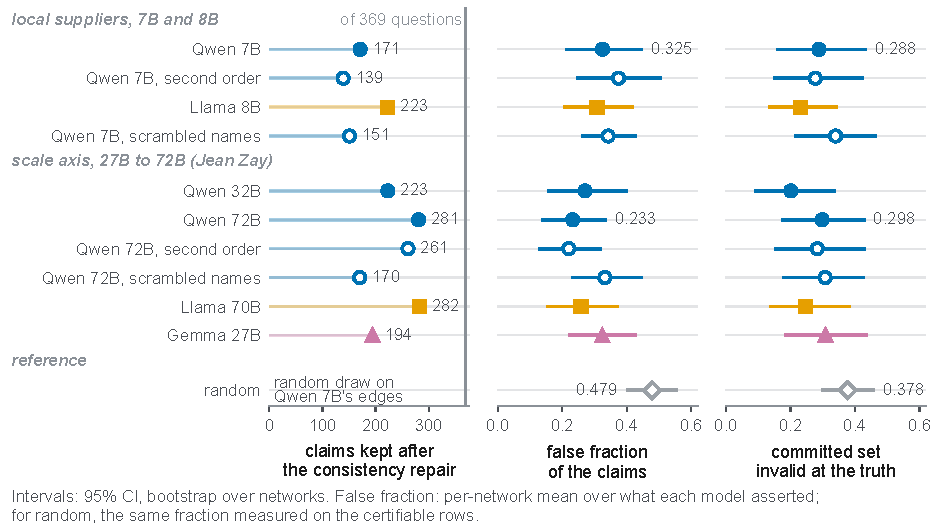
\includegraphics[width=\linewidth,height=0.25\textheight,keepaspectratio]{supplier_scale.pdf}
\caption{Scale buys claims and accuracy per claim, not validity: across the Qwen family the number of
kept claims rises from 171 to 223 to 281 and the false fraction falls, while the share of certifiable
rows whose committed set is invalid at the truth goes 0.288, 0.201, 0.298, in no order and with
overlapping intervals.}
\label{fig:supplier-scale}
\end{figure}

The mechanism is counting. A set is invalid when one wrong claim sits where the query needs it, and a
supplier that asserts more puts more claims near each query. On commission, gemma is the high outlier
against the 72B.
At 72B the model is also far more stable under presentation order: instrument disagreement
\textbf{0.047} [0.019, 0.079] on shared edges, against 0.160 at 7B (\texttt{TABLE4.md}). The batch
script is \texttt{experiments/remote/elicit\_jz.slurm} (one node, four H100, every cache on scratch
because vLLM's compile cache overflowed the home quota, eager mode); \texttt{elicit\_import.py} puts the
answers under the local cache key, and \texttt{elicit\_run.py} refuses to call a cluster model.


\prompt[conceito=escala-validade,dificuldade=0.7]{Without numbers: why can a supplier that is wrong
less often per claim leave the committed set invalid just as often?}{A committed set is invalid when at
least one wrong claim sits where the query needs it. The larger model declines far less, so it asserts
more edges in each component and more queries become certifiable; every extra claim near a query is
another chance that one of them is wrong. A lower rate per claim times more claims per query leaves the
chance of at least one wrong claim where it was. Accuracy per claim and validity per query are
different quantities, and the certificate sits between them.}

% -----------------------------------------------------------------------------
\begin{antes}
\antesq[sobreposicao-fonte]{Asked cold for the publication behind each network, how many do the local
suppliers name?}
\antesq[ponte-compelida]{Is the error on compelled edges, which needs no truth, an unbiased estimate of
commission on open edges?}
\end{antes}

\section{Names, a truth-free bridge, and two negative results}\label{sec:sup-names}

\emph{Scrambled names.} At 7B, scrambling gives commission 0.343 [0.260, 0.431] against 0.325; what
changes is declining, omission 0.568 against 0.450 (L3 not supported). At 72B the gap is $+0.088$
[$-0.064$, $+0.238$] and the model declines 96 pairs against 27 (S3). A source reciting the benchmarks
would collapse without the names, and neither does; by invariance, that licenses ``no recitation
detected'' and nothing stronger.

\emph{The compelled-edge bridge.} The control block asks about edges the data already orient, so its
error needs no truth. If it estimated open-edge commission without bias, a tier with no known truth
could be scored. At 7B it does not: 0.191 [0.094, 0.293] against 0.325, a correction of about 0.13 that
varies by network (L9 not supported).

\begin{medido}[Control minus open-edge commission, \texttt{results/elicit/knowledge\_audit.json}]
Paired by network: 7B \textbf{$-0.153$} [$-0.324$, $+0.009$] on 23 networks; 72B \textbf{$+0.004$}
[$-0.153$, $+0.159$] on 26. The 72B's own control error is 0.232 [0.121, 0.358], higher than the 7B's
0.191, so size did not improve the control; it removed the bias. At 7B the paired interval reaches
$+0.009$: the bias rests on the registered comparison and a point estimate of $-0.15$.
\end{medido}

The bridge is therefore reported per supplier: usable at 72B, biased at 7B.

\emph{The source-overlap probe.} The scrambled arm answers the recitation question only by invariance,
so a second probe asks it directly: shown the variable list alone, name the publication behind the
network and its declared exposure, outcome and adjustment set. ``Recited'' requires the source and the
query.

\begin{medido}[Source overlap, \texttt{results/elicit/SOURCE\_OVERLAP.md}]
32 networks, 29 with a scorable source, 10 with a declared query. Source named: \textbf{0 of 29} for
\texttt{qwen2.5:7b}, which declines on 28 and misattributes the one it answers; \textbf{0 of 29} for
\texttt{llama3.1:8b}, which answers all 29 and matches none. Declared query reproduced on 2 of 10 by
each, never with the source. \textbf{Recited: none}, for both.
\end{medido}

Matching a query without the source is reading the names. The pre-registration's appendix scores an
earlier pass on prompts rendered with the salted seed of Chapter~\ref{ch:frame} (27 declines, same
verdict); the box is the rerun on stable prompts. The cluster models have not been probed.

\emph{Ancestral claims.} Asked about 156 non-adjacent pairs at skeleton distance two, the 7B asserted
ancestry on \textbf{6}, said ``neither'' on 45 and declined 105; the six reduce soundly to ten
orientations, four false, which change one true claim on one swept network and no certificate
(\texttt{results/elicit/PREREGISTRATION\_ANCESTRAL.md}). All three predictions fell: a negative result.

\prompt[conceito=ponte-compelida,dificuldade=0.75]{At which supplier size is the compelled-edge bridge
unbiased, what is the number, and why does that not mean the larger model is better on compelled
edges?}{At 72B: control minus open-edge commission $+0.004$ [$-0.153$, $+0.159$], paired over 26
networks, against $-0.153$ [$-0.324$, $+0.009$] at 7B. The 72B's error on compelled edges is 0.232,
higher than the 7B's 0.191; the bridge is unbiased because its control error and its open-edge
commission now agree, not because the control error fell.}

% -----------------------------------------------------------------------------
\begin{antes}
\antesq[teste-cascata]{Does the greedy recovering set, which the old pipeline used as knowledge,
orient more edges per claim than the 7B supplier?}
\antesq[teste-cascata]{Which justification for the redesign was withdrawn, and what still carries it?}
\end{antes}

\section{The cascade test: a justification withdrawn}\label{sec:sup-cascade}

The committed pipeline's knowledge was the greedy recovering set, now \texttt{A\_ORACLE}: few claims,
chosen from the truth so that Meek's closure recovers as much as possible. The redesign had two reasons
to drop it: the invariant, and ``the old generator cascades unrealistically'', registered to be
withdrawn unless the oracle set compels more edges per claim than an elicited set, paired by network.

\begin{exemplo}[Three sources on \texttt{child}]
The 7B keeps one claim, the false \texttt{CO2} $\to$ \texttt{LungParench} of Chapter~\ref{ch:frame},
and the closure orients 10 edges the CPDAG left open. The oracle set asserts 2 and orients 12; the 72B
asserts 8 and orients 9. Per claim: 10, 6 and 1.125. The same edge oriented truthfully,
\texttt{LungParench} $\to$ \texttt{CO2}, orients 2 (\texttt{results/ledger/rows.csv}, columns
\texttt{n\_k} and \texttt{k\_g0}). On this network the 7B cascades most.
\end{exemplo}

The quantity is \emph{closure per claim}, $k_{\Gz}/|\Kset|$: edges the analyst's graph orients that
$\Chat$ left open, asserted or propagated, over kept claims. It is constant within a network and an arm,
so the test pairs arms by network (\texttt{experiments/cascade\_test.py}).

\begin{medido}[Cascade test, \texttt{results/ledger/cascade\_test.json}]
Oracle $-$ 7B: \textbf{$+1.13$} [$-0.26$, $+2.86$] on 27 networks, larger on 14: \textbf{not
separated}. Oracle $-$ 72B: $+1.28$ [$+0.43$, $+2.50$]; oracle $-$ Llama 70B: $+1.62$ [$+0.32$,
$+3.27$]; both separated. Truthful orientations on the 7B's edges $-$ 7B: $-0.63$ [$-1.52$, $-0.02$].
Network means: oracle 2.97, 7B 1.84, 70B 1.35, 72B 1.15.
\end{medido}

The justification is withdrawn as written (\texttt{results/ledger/CHECKS.md}). \figref{fig:cascade}
shows why ``unrealistic'' had no fixed referent: the 7B declines a lot, keeps few claims, and each drags
others along, as the oracle's minimal set does; the large models assert almost every edge of a
component, and then the closure has little left to add.

\begin{figure}[htbp]
\centering
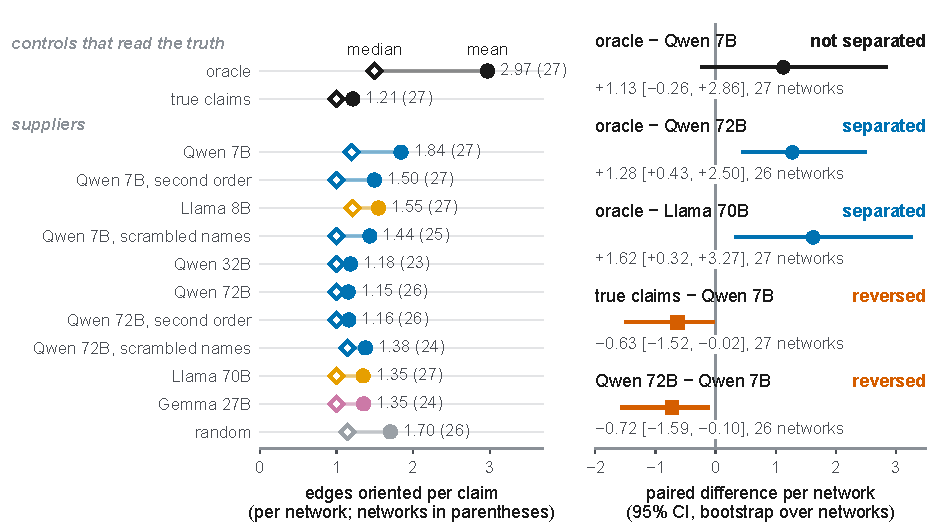
\includegraphics[width=\linewidth,height=0.22\textheight,keepaspectratio]{cascade.pdf}
\caption{Whether the old generator ``cascades too much'' depends on the supplier it is compared with:
the oracle set does not separate from the 7B supplier in edges oriented per claim, and does separate
from the 72B and 70B suppliers, which assert many claims that propagate little. The redesign keeps
only the invariant as its reason.}
\label{fig:cascade}
\end{figure}

\prompt[conceito=teste-cascata,dificuldade=0.7]{Explain without contradiction why the same oracle set
does not cascade more than the 7B supplier but does cascade more than the 72B.}{Closure per claim
depends on how much a source says. The 7B declines a lot (137 of 369 pairs) and keeps few claims per
component, and each drags orientations along through Meek's rules, as the oracle's minimal set does.
The 72B keeps claims on almost every pair (281 of 369); when nearly every edge of a component is asserted
directly, the closure adds little and the ratio is close to 1. ``Unrealistic'' only means something
against a reference source, and the real sources disagree with each other.}

\naopasse[escala-validade]{Write the chain from ``the 72B keeps 281 claims'' to ``its set is invalid
on 0.298 of certifiable rows''. If the step from more claims to more invalid sets does not come, reread
Section~\ref{sec:sup-scale}.}

\begin{exercicio}[metodo=table-reading,conceito=escala-validade]
From \texttt{TABLE4.md} and \texttt{knowledge\_audit.json}, the six real-name suppliers at the first
order. (a) Within the Qwen
family, does the invalid-set rate fall with size? (b) Which column explains gemma? (c) Check that the
first four columns account for all 369 pairs for the 72B and for Llama 70B. (d) Which supplier is
``best'', and why does that question not belong in the paper?

\begin{center}
\small
\begin{tabular}{@{}lrrrrrrr@{}}
\toprule
supplier & kept & dropped & declined & not reached & commission & certifiable & invalid \\
\midrule
Qwen 7B   & 171 & 43 & 137 & 18 & 0.325 & 229 & 0.288 \\
Qwen 32B  & 223 & 26 &  83 & 37 & 0.271 & 204 & 0.201 \\
Qwen 72B  & 281 & 24 &  27 & 37 & 0.233 & 285 & 0.298 \\
Llama 8B  & 223 & 41 &  92 & 13 & 0.308 & 243 & 0.230 \\
Llama 70B & 282 & 78 &   9 &  0 & 0.259 & 267 & 0.247 \\
gemma 27B & 194 & 68 &  14 & 93 & 0.324 & 263 & 0.308 \\
\bottomrule
\end{tabular}
\end{center}
\end{exercicio}
\begin{solucao}
(a) No: 0.288, 0.201, 0.298, in no order, and Table~4's intervals overlap. (b) ``Not reached'': gemma
leaves 93 pairs unanswered, drops 68 in the repair and keeps a commission as high as the 7B's.
(c) 72B: $281 + 24 + 27 + 37 = 369$. Llama 70B: $282 + 78 + 9 + 0 = 369$. (d) None: the suppliers are
error sources for testing instruments, and what the paper uses is that validity does not improve with
scale.
\end{solucao}

\begin{exercicio}[metodo=estimation,conceito=escala-validade]
Model a certifiable row as depending on $m$ claims, each false independently with probability equal to
the supplier's commission $c$, so the set is invalid with probability $1 - (1-c)^m$. (a) Estimate the
effective $m$ that reproduces the invalid-set rate for the 7B ($c = 0.325$, rate 0.288) and for the 72B
($c = 0.233$, rate 0.298). Use $\ln 0.675 \approx -0.393$, $\ln 0.712 \approx -0.340$,
$\ln 0.767 \approx -0.265$, $\ln 0.702 \approx -0.354$. (b) Compare the ratio of the two $m$ with the
ratio of pairs the two suppliers kept. (c) Name two reasons the model is too crude to report.
\end{exercicio}
\begin{solucao}
(a) 7B: $m = \ln 0.712 / \ln 0.675 \approx 0.340/0.393 \approx 0.86$. 72B: $m = \ln 0.702 / \ln 0.767
\approx 0.354/0.265 \approx 1.33$. (b) $1.33/0.86 \approx 1.5$, against $281/171 \approx 1.6$ kept
claims: the rise in effective claims per query is about the rise in claims, which is the counting
mechanism in numbers. (c) Errors are not independent (one answer, one repair, clustering by network); validity
depends on the claims on the query's paths, not on a random $m$; and the rates come from different
certifiable rows, 229 and 285. An order-of-magnitude check, not a result.
\end{solucao}

\section*{Chapter map}

\begin{center}
\begin{tikzpicture}[x=1cm, y=1cm]
\node[cmap]  (q)  at (0, 0)      {four knowledge processes};
\node[cmapc] (f)  at (4.15, 0)   {knowledge suppliers as error processes};
\node[cmap]  (co) at (8.3, 0)    {commission and omission, never summed};
\node[cmap]  (b)  at (12.45, 0)  {compelled-edge bridge, per supplier};
\node[cmapr] (v)  at (0,-1.7)    {validity does not improve (S6)};
\node[cmap]  (e)  at (4.15,-1.7) {scale, 7B to 72B};
\node[cmapr] (c)  at (8.3,-1.7)  {cascade justification withdrawn};
\node[cmapg] (s)  at (12.45,-1.7) {no recitation: source named 0 of 29};
\draw[cedge] (q) -- node[above] {one of them} (f);
\draw[cedge] (f) -- node[above] {scored by} (co);
\draw[cedge] (co) -- node[above] {bias test} (b);
\draw[cedge] (f) -- node[left] {varied by} (e);
\draw[cedge] (e) -- node[above] {more claims} (v);
\draw[cedge] (e) -- node[above] {7B ties} (c);
\draw[cedge] (f.south east) -- node[above, sloped, pos=0.75] {probed by} (s.north west);
\end{tikzpicture}
\end{center}

% =============================================================================
\chapter[Table 4: the claim unit never over-certifies, the hop unit does]{Table 4: the claim unit\\ never over-certifies, the hop unit does}\label{ch:table4}

Table~4 is the audit that closes the protocol run. On every certifiable row it asks each instrument
one question: when you promised that $r-1$ revisions were safe, had the analyst already made more
wrong claims than that, on a set that was invalid? This chapter reads
\texttt{results/ledger/TABLE4.md}, shows why the claim radius's zero is a consequence and not an
estimate, and tells what the pre-registered inspection trigger found on 12 September. Three findings
touch code in your repository; I state each one as exactly as I can.

\begin{antes}
\antesq[baldes]{A radius promises that $r-1$ revisions are safe. Against which two facts, known only
to the truth, does the audit check that promise?}
\antesq[distancia-em-saltos]{On the \texttt{child} row of this section, how many claims and how many
covering hops separate $\Gz$ from the first state where the committed set fails?}
\end{antes}

\section{The ledger, five instruments and four buckets}

\begin{ideia}
A radius is a promise: you may be wrong in up to $r-1$ of your moves and the adjustment set still
holds. The audit checks it against the two things only the truth knows, the number $w$ of asserted
claims that are false and whether $Z$ is valid; two yes-or-no answers give four buckets.
\end{ideia}

The ledger crosses the frozen frame of Chapter~\ref{ch:frame} with every knowledge condition of
Chapter~\ref{ch:suppliers}.

\begin{medido}[The ledger, \texttt{results/ledger/sweep\_summary.json} and \texttt{TABLE4.md}]
528 frame rows on 27 networks, 14 knowledge conditions, 8,308 evaluations by
\texttt{experiments/ledger\_sweep.py}. The eleven deployment conditions that assert knowledge (the 7B
primary supplier with its order and scrambled-name replicates, the 8B second family, six conditions on
four larger checkpoints, chance with three draws) certify \textbf{3,014} rows; no knowledge certifies
68, none invalid at the truth; the two audit conditions, which read the truth, 503. The primary
supplier \texttt{D\_LLM} (qwen2.5 7B, real names) certifies 229 of 528; on 155 its own graph reverses
the query, and 144 are not amenable.
\end{medido}

Every CPDAG in the ledger is the true DAG's (stamp \texttt{via\_Chat\_only}); Chapter~\ref{ch:pest}
removes that idealisation. Five instruments answer from observables alone.

\begin{center}\small
\begin{tabular}{@{}p{3.75cm}p{11.75cm}@{}}
\toprule
free rule (B2) & hop distance inside $X$'s chain component to the nearest member of $Z$; 1 when none
is there \\
closure count $k_{\Gz}$ (B4) & orientations of $\Gz$ absent from $\Chat$, asserted and propagated \\
claim count $|\Kset|$ (B5) & number of claims \\
hop radius $\rhop$ (B6) & your $\rval$ as \texttt{hybrid.breakdown\_radius} computes it: fewest covering
hops up from $\Gz$ to a failing state; a floor when the walk is budgeted \\
claim radius $\rclaim$ (B7) & fewest claims whose retraction and re-closure make $Z$ fail, exhaustive to
depth 3 under 300 subsets; a floor when censored \\
\bottomrule
\end{tabular}
\end{center}

\begin{exemplo}[\texttt{child}, LungParench $\to$ Grunting, primary supplier]\label{ex:child}
One claim, CO2 $\to$ LungParench, and it is false ($w = 1$). Meek's rules turn it into ten
orientations: LungParench $\to$ Disease, seven edges out of Disease (Sick among them), LVH $\to$
LVHreport. In $\Gz$ Disease is a mediator and the committed set $Z = \emptyset$ is valid; in the truth
Disease causes both LungParench and Sick, and $\emptyset$ leaves that path open.

\begin{center}
\begin{tikzpicture}[x=1cm,y=1cm,
  nd/.style={nodot, font=\scriptsize\sffamily},
  st/.style={blk, font=\tiny\sffamily, align=center, text width=2.2cm, inner sep=2pt},
  stf/.style={blkr, font=\tiny\sffamily, align=center, text width=2.2cm, inner sep=2pt},
  lab/.style={font=\tiny\sffamily, text=cinzaescuro}]
\node[font=\scriptsize\sffamily\bfseries] at (1.6,0.95) {$\Gz$: one claim, false};
\node[nd] (c) at (0,0.3) {CO2};
\node[nd] (l) at (1.6,0.3) {LungParench};
\node[nd] (g) at (3.3,0.3) {Grunting};
\node[nd] (d) at (1.6,-0.9) {Disease};
\node[nd] (s) at (3.3,-0.9) {Sick};
\draw[falsa] (c) -- (l);
\draw[aresta] (l) -- (g);
\draw[propagada] (l) -- (d);
\draw[propagada] (d) -- (s);
\draw[aresta] (s) -- (g);
\node[font=\tiny\sffamily, text=azulesc] at (1.6,-1.45) {+ 7 more propagated};
\begin{scope}[xshift=4.5cm]
\node[font=\scriptsize\sffamily\bfseries] at (1.6,0.95) {the truth};
\node[nd] (c) at (0,0.3) {CO2};
\node[nd] (l) at (1.6,0.3) {LungParench};
\node[nd] (g) at (3.3,0.3) {Grunting};
\node[nd, draw=vermesc] (d) at (1.6,-0.9) {Disease};
\node[nd] (s) at (3.3,-0.9) {Sick};
\draw[aresta] (l) -- (c);
\draw[aresta] (l) -- (g);
\draw[aresta] (d) -- (l);
\draw[aresta] (d) -- (s);
\draw[aresta] (s) -- (g);
\node[font=\tiny\sffamily, text=vermesc] at (1.6,-1.45) {$Z=\emptyset$ invalid};
\end{scope}
\begin{scope}[xshift=9.3cm]
\node[st, text width=2.6cm] (g0) at (2.5,0.8) {$\Gz$: 10 orientations; $\emptyset$ valid};
\node[st] (h1) at (1.15,-0.35) {drop the claim, keep its 9; $\emptyset$ valid};
\node[stf] (h2) at (1.15,-1.45) {also drop LungPar.\,$\to$\,Disease; fails};
\node[stf] (ch) at (4.1,-0.35) {back to $\Chat$; $\emptyset$ fails};
\draw[flow] (g0.south west) ++(0.35,0) -- node[lab, left, pos=0.45] {hop 1} (h1.north);
\draw[flow] (h1) -- node[lab, left] {hop 2} (h2);
\draw[flow] (g0.south east) ++(-0.35,0) -- node[lab, right, pos=0.45] {1 claim} (ch.north);
\end{scope}
\end{tikzpicture}
\end{center}

Retracting the claim returns to $\Chat$, where $\emptyset$ fails: $\rclaim = 1$. The hop walk moves one
orientation at a time; its only first step keeps the nine propagated orientations, a closed state
nobody asserted, and only the second step breaks $Z$: $\rhop = 2$. Free rule, closure count, claim
count,
hop and claim radius certify 1, 10, 1, 2, 1 (\texttt{results/ledger/rows.csv}); covering $w = 1$ needs
$r \ge 2$, so the closure count and the hop radius promise safety on a broken set.
\end{exemplo}

Every instrument is scored against $w$ counted in claims, since claims are what the analyst asserted.
In its own unit the hop radius is right; the danger is hearing «one revision is safe» as «one wrong
claim is safe», when undoing this one wrong claim takes ten orientations.

\begin{formulabox}[The buckets, \texttt{experiments/ledger\_sweep.py}, function \texttt{bucket}]
An instrument certifies $r$ on a row with $w$ false claims. It \emph{covers} the row iff $r = \infty$ or
$w \le r-1$. \textbf{dangerous}: covers, $Z$ invalid at the truth; \textbf{held}: covers, valid;
\textbf{safe}: does not cover, invalid; \textbf{slack}: does not cover, valid. Dangerous rate over
certifiable rows; detection = safe over invalid rows; false alarm = slack over valid rows. A budgeted
search enters with the floor it certifies (\texttt{claim\_lower\_bound}), never as $\infty$.
\end{formulabox}

Dangerous is the verdict an analyst cannot recover from; slack is a refused move that was fine. So
validity is read as absolute and sharpness only among safe instruments, as one reads a conformal
method: coverage first, size second.

\prompt[conceito=baldes,dificuldade=0.65]{Explain to yourself, then check: why can a row on which no
retraction breaks $Z$ ($r = \infty$) only be held or dangerous, and what would a dangerous row of that
kind mean for the claim radius?}{Because $r = \infty$ covers every $w$, so only validity at the truth
separates held from dangerous. For the claim radius such a row contradicts the proposition of
Section~\ref{sec:t4-why} as long as the class is correct: retracting the $w$ false claims leaves a graph
the truth extends, where an invalid $Z$ must fail, so some retraction would have broken $Z$. The row
is a code defect or a violated premise, which is what the inspection trigger of
Section~\ref{sec:t4-trigger} exists to separate.}

% -----------------------------------------------------------------------------
\begin{antes}
\antesq[fornecedor-conhecimento]{Is the primary supplier better than chance at what it asserts, and is
its committed set invalid less often?}
\antesq[baldes]{On how many deployment rows is each of the free rule, the hop radius and the claim
radius dangerous, and over which population?}
\end{antes}

\section{What Table 4 says}

\begin{medido}[Table 4, blocks 1 and 2, \texttt{results/ledger/TABLE4.md}]
Primary supplier, 229 certifiable rows: false claims over asserted \textbf{0.329} [0.184, 0.494]; set
invalid at the truth \textbf{0.288} [0.155, 0.435], 66 rows. Chance on the same edges, 649 rows: 0.479
[0.398, 0.559] and 0.378 [0.295, 0.460]. Paired on 24 networks, chance minus supplier, post hoc: +0.143
[+0.006, +0.287] and +0.082 [$-$0.020, +0.176]. Network cluster bootstrap, $B = 4000$. The false-claim
rate here is over the 229 certifiable rows on 27 networks; Chapter~\ref{ch:suppliers} quotes 0.325
[0.210, 0.449], the network mean over all kept claims on 32 networks (\texttt{results/elicit/knowledge\_audit.json}).
Both are right for their population.
\end{medido}

The supplier beats a coin on what it says, in a contrast declared afterwards; on whether the set breaks
the difference is not shown. L4 asked for separated intervals and did not get them, so the abstract
leads
with the identifiability step (68 certifiable rows without knowledge, 229 with it) and with the
dangerous
counts, each of which needs its population.

\begin{medido}[Dangerous rows, \texttt{TABLE4.md} ladder block, recounted from \texttt{rows.csv}]
\centering\small
\begin{tabular}{@{}lcccc@{}}
\toprule
& primary supplier & five conditions, 12 Sep & eleven conditions & audit conditions \\
certifiable rows & 229 & 1,524 & 3,014 & 503 \\
\midrule
free rule & 0 & 15 & 15 & 0 \\
hop radius & 4 & 29 & 39 & 0 \\
claim radius & \textbf{0} & \textbf{0} & \textbf{0} & 0 \\
\bottomrule
\end{tabular}\\[0.3em]
\raggedright
The five conditions of 12 September: primary supplier, order replicate, second family, scrambled names,
chance. There the closure count is dangerous on 0.22 to 0.34 of rows, the claim count on 0.17 to 0.34.
The audit zeros hold by construction ($w = 0$, true claims keep $Z$ valid) and never enter a sentence
about instruments.
\end{medido}

On the primary supplier the free rule and the claim radius are both safe, so what separates them is
sharpness. \figref{fig:buckets} shows it bucket by bucket, and the paired ladder measures it.

\begin{figure}[tbp]
\centering
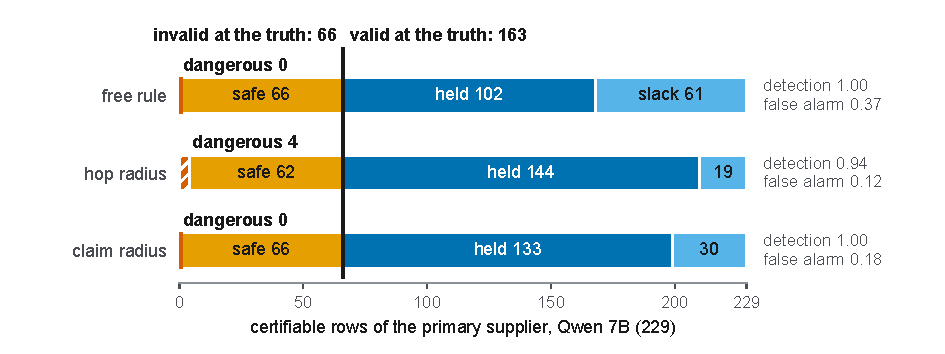
\includegraphics[width=\linewidth]{buckets_7b.pdf}
\caption{Safety is read left of the rule and sharpness right of it. Of the 66 sets invalid at the
truth, only the hop radius leaves any in the dangerous bucket. Of the 163 valid sets, the claim radius
refuses a move on 30 and the free rule, equally safe on this supplier, on 61.}
\label{fig:buckets}
\end{figure}

\begin{medido}[The paired ladder, \texttt{TABLE4.md}, last block]
False alarm, claim radius minus the other instrument, difference of network means on the same rows.
Against the free rule: primary supplier \textbf{$-$0.206} [$-$0.380, $-$0.053] on 25 networks, radius
wins; order replicate $-$0.188, scrambled $-$0.246, chance $-$0.308, wins; second family $-$0.129
[$-$0.294, +0.038], underpowered; the six scale-axis conditions $-$0.19 to $-$0.27, six wins. Against
the
hop radius: primary supplier \textbf{+0.144} [+0.025, +0.297], radius loses; +0.12 to +0.19 on the other
four conditions of 12 September.
\end{medido}

Appendix A.2 of \texttt{results/ledger/PREREGISTRATION.md} writes the abstract from one sentence: the
free rule is safe and blunt, the hop radius sharp and unsafe, the claim radius safe and sharper than the
safe alternative. Its errata of 13 September qualify «safe» for the free rule, strict only on the
primary
supplier and the scale axis and dangerous on 3 to 6 rows in each of the other four conditions.

\prompt[conceito=fornecedor-conhecimento,dificuldade=0.75]{Is the primary supplier better than chance?
Answer on both measures with the numbers, and say what the pre-registration asked.}{On false claims
yes, but only in a post hoc paired contrast: chance is +0.143 [+0.006, +0.287] higher on 24 networks
(0.479 against 0.329). On sets invalid at the truth it is not shown: +0.082 [$-$0.020, +0.176] (0.378
against 0.288). L4 asked for separated intervals and is not supported as registered, so the elicited
condition is reported as not shown to be informative on this substrate.}

% -----------------------------------------------------------------------------
\begin{antes}
\antesq[unidade-afirmacao]{Why does the claim radius's zero get no confidence interval?}
\antesq[gac-backdoor]{Do the claim radius and the hop radius in the ledger decide validity with the
same criterion?}
\end{antes}

\section{Why the zero is structural, and what the hop rows are}\label{sec:t4-why}

More rows would not tighten the zero. It follows from one move: retracting exactly the false claims.

\begin{proposicao}[The claim radius cannot over-certify, given a correct
class]\label{prop:t4-structural}
Let $Z$ be committed in $\Gz = \mathrm{Meek}(\Chat, \Kset)$, let certificate and audit decide validity
with the same generalised adjustment criterion, and suppose the true DAG belongs to the class of
$\Chat$. If $Z$ is invalid at the truth and the false claims form $W \subseteq \Kset$, $|W| = w$, then
retracting $W$ breaks $Z$. Hence $\rclaim \le w$ whenever the search reaches depth $w$, every floor
certified below depth $w$ is at most $w$, and the claim radius never covers $w$.
\end{proposicao}

\noindent\emph{Proof.} The claims in $\Kset \setminus W$ are true and the truth is in the class of
$\Chat$, so the truth extends $\mathrm{Meek}(\Chat, \Kset \setminus W)$. Validity in an MPDAG is
validity
in every extension, and $Z$ fails in this one. \hfill$\square$

The zero is what a sound criterion and an audit asking the same question must return, so it gets no
interval; the rule-of-three floor Table~4 prints beside it (0.0131 for the primary supplier, $3/229$)
would turn a consequence into a rate. Reading the radius as a minimal correction set needs failure to be
upward-closed under retraction, your Theorem~1, and that was audited as implemented.

\begin{medido}[Monotonicity, \texttt{experiments/monotonicity\_audit.py}]
5,000 pairs (a failing retraction set, a random superset) on 469 rows of the elicited, truthful and
oracle conditions: \textbf{0 violations}; one-sided 95\,\% bound 0.0006, treating pairs as independent
although they cluster within rows (\texttt{results/ledger/monotonicity\_audit.json}). Proposition~1 of
your draft rests on this theorem.
\end{medido}

The hop radius's dangerous rows are where the two units part.

\begin{medido}[The unit gap, \texttt{PREREGISTRATION.md} A.0b and A.2, recounted from \texttt{rows.csv}]
Of the hop radius's 29 dangerous rows on the five conditions of 12 September, \textbf{22} have
$\rclaim = 1$, $\rhop = 2$, one false claim and an invalid set, the shape of Example~\ref{ex:child}; of
its 39 on all eleven conditions, 28. Leverage $\rhop/\rclaim$ on the 1,390 rows of the 12 September
ledger with both radii exact and finite: median 1, above 5 on 8 rows, maximum 12 (oracle) and 9
(deployment).
\end{medido}

One confound had to be ruled out before quoting the gap, and I found it only while writing this chapter.

\begin{armadilha}[Two criteria inside one ladder]
In the ledger the claim radius decides failure with the generalised criterion,
\texttt{is\_gac\_valid\_mpdag}
in \texttt{src/bkrobust/gac/mpdag\_level.py}. The hop radius, through \texttt{breakdown\_radius}, uses
\texttt{is\_valid\_mpdag} in \texttt{src/bkrobust/mpdag\_criterion/criterion.py}, which carries the
back-door strengthening. Your \texttt{THEOREMS.md} §13 gives the direction, $\rval(\text{GAC}) \ge
\rval(\text{back-door})$, so a GAC
hop radius would be dangerous on at least the same rows and raise no more false alarms. Both hop
conclusions are conservative; the columns should still share one criterion before the paper sets them
side by side.
\end{armadilha}

For your draft, this is the measurement behind the abstract's distance that «counts elementary revisions
of the analyst's own claims». An elementary revision is a covering step, which on every case checked
changes exactly one orientation, propagated or asserted alike (\texttt{THEOREMS.md}, Lemma~R). Read as a
count of wrong claims, the hop radius over-certified on 39 of 3,014 rows where the claim radius never
did. Chapter~\ref{ch:merge} takes up the unit the paper reports in.

\begin{sonorio}[The licensed form, for the audit table]
\emph{On the 3,014 certifiable queries of eleven elicited and chance knowledge conditions, on the true CPDAG, the claim radius never
certified more wrong claims than the analyst had made on an invalid adjustment set, which a sound
criterion guarantees when the equivalence class is correct. Counted in covering hops, the radius did so
on 39 queries, and the free hop-count rule on 15. Where the free rule was also safe, the claim radius
raised fewer false alarms.} Never: an interval on the zero, «robust», «in deployment», «beats a
leave-$k$-out screen» (Chapter~\ref{ch:m1b}).
\end{sonorio}

\prompt[conceito=unidade-afirmacao,dificuldade=0.75]{State the move that makes the claim radius's zero
structural, its premise, and why the rule-of-three column must not be quoted as its bound.}{Retract
exactly the $w$ false claims: the rest are true, so if the truth is in the class of $\Chat$ it extends
the re-closed graph, where an invalid $Z$ fails, giving $\rclaim \le w$ (and any censored floor below
depth $w$ is at most $w$). The premise is a correct class, with certificate and audit on one criterion.
The zero is a consequence, not a frequency: a bound like $3/229 = 0.0131$ describes a rate that more
rows
could tighten, while this zero fails only when the premise does.}

\prompt[conceito=gac-backdoor,dificuldade=0.8]{In the ledger the two radii decide failure with different
predicates. Which ones, and why can that not have produced any of the 39 dangerous hop rows?}{The claim
radius uses \texttt{is\_gac\_valid\_mpdag}, the generalised criterion; the hop radius uses
\texttt{mpdag\_criterion.is\_valid\_mpdag}, with the back-door strengthening. Back-door validity implies
GAC validity (\texttt{THEOREMS.md} §13), so back-door failure comes no later and that hop radius is
never
larger than a GAC one. A larger radius covers more, so a GAC hop radius would be dangerous on at least
the same rows.}

% -----------------------------------------------------------------------------
\begin{antes}
\antesq[gatilho-inspecao]{What does the clause attached to L6 order when one dangerous row of the claim
radius appears, and what does it forbid until then?}
\antesq[orcamento-retracao]{A claim search stopped by its 300-subset budget: what did it certify?}
\antesq[gac-backdoor]{Which function in your repository is Pearl's back-door criterion, and which test
now pins where it differs from the generalised criterion?}
\end{antes}

\section{The inspection trigger fired}\label{sec:t4-trigger}

L6 predicted no dangerous row for the claim radius, and the clause beside it said: one such row, halt
and inspect it before reading anything else, because it is a bug or the result. The first complete
table showed seven, six under the order replicate and one under the second family, and 29 for the hop
radius (\texttt{PREREGISTRATION.md}, A.0b). The inspection found two bugs and one result.

\paragraph{Six rows: a floor read as infinity.} All six are on \texttt{paths}, the 17-node textbook network (its chain component holds 15 nodes)
chain, where the order replicate asserted 13 claims, all false. The search stops before exceeding 300
subsets: $13 + 78 = 91$, and size three would add 286, so it stops at \texttt{censored\_at\_depth\_3},
certifying $\rclaim \ge 3$. That floor covers two wrong claims against $w = 13$: safe. The first bucket
function scored the censored radius as unbounded, hence dangerous. Every censored radius now enters at
its floor, and a search that tried every subset without a failure is stamped \texttt{unreached} instead
of \texttt{gt\_d}. The six rows are still in \texttt{rows.csv}, now safe; the ledger holds 66 rows
censored at depth 3 and 3 at depth 2.

\paragraph{One row: the audit asked a different question.} On \texttt{ecoli70}, second family, query
yedE $\to$ b1963: four claims, three false (nmpC $\to$ pspA, pspA $\to$ cspG, pspA $\to$ pspB),
committed
set $\{\text{atpD}, \text{pspA}\}$. The certificate found no break up to depth three; the audit called
the set invalid. By the proposition both cannot hold, since the three false claims were a subset the
search tried. An independent implementation of the generalised criterion on \texttt{networkx} sided with
the certificate. The audit had used \texttt{is\_valid\_adjustment\_set\_dag}
(\texttt{src/bkrobust/demo/evaluate.py}), which is Pearl's back-door criterion and says so in its
docstring: it forbids every descendant of the treatment, and pspA descends from yedE on no causal path
to
b1963. Your \texttt{THEOREMS.md} §13 and §14 already state the relation (the generalised criterion
accepts a superset and coincides on $\Ostar$). The error was ours, in choosing that function for the
audit.

\begin{medido}[The oracle, \texttt{PREREGISTRATION.md} A.0b, recounted from \texttt{rows.csv}]
On the 1,169 committed sets of the four elicited conditions of 12 September and the oracle condition,
the back-door function rejected \textbf{4} that the generalised criterion accepts, each holding a
descendant of the treatment off every causal path, and agreed on the other 1,165. On all 3,585
certifiable rows of the current ledger: 6, always in that direction.
\end{medido}

Your function was not touched. The audit calls \texttt{is\_valid\_adjustment\_set\_gac\_dag} in
\texttt{src/bkrobust/benchmarks/audit.py}, which shares no code with the instrument, and keeps the
back-door verdict as the column \texttt{z\_backdoor\_at\_truth}. The guard test
\texttt{tests/\allowbreak benchmarks/\allowbreak test\_audit\_oracle.py} pins the smallest case: $U
\to X \to C \to Y$, $U \to Y$,
$X \to A$, where $\{U, A\}$ is valid under the generalised criterion and rejected by the back-door
function, while all three oracles agree on $\{U\}$, $\emptyset$, $\{C\}$, $\{U, C\}$. The 29 hop rows
showed no defect: they are the unit gap, and they stayed. The sweep was rerun with the two fixes and
nothing else.

A zero reached by fixing code is suspect by default. This one rests on checkable facts: the halt clause
predates the first row, each fix is recorded in A.0b with the row that triggered it and a reason
independent of the outcome, the unwelcome hop rows were left alone, and the next fix (the severity
label)
was rerun and diffed, changing only that column on 113 of 5,140 rows.

\begin{digressao}[The ladder that never returned]
The first sweep hung on \texttt{andes} (223 nodes) inside the CP-SAT ladder: \texttt{add\_failure}
(\texttt{src/bkrobust/sat/failure.py}) loops, at each of the path's node positions, over every ordered
node triple, about $2.4 \times 10^{9}$ iterations at 223 nodes against $1.2 \times 10^{7}$ at 60. The
5-second limit bounds the solver, not the build, which had not returned after twelve minutes; those rows
were discarded unread (A.0). The hop walk is now exhaustive up to 12 retractable edges and depth 3
beyond,
under 4,000 closures, the ladder runs only up to 60 nodes, and a budgeted walk enters the bucket as
$\rhop \ge \text{depth}+1$. The gate is a workaround; the build itself is unchanged.
\end{digressao}

\naopasse[gac-backdoor]{Write the three facts that made the \texttt{ecoli70} row a contradiction: how
many claims were false, how deep the search went, and what that implied for $\rclaim$ if $Z$ were
invalid. If one is missing, reread that paragraph before the exercises.}

\begin{exercicio}[metodo=diagnosis,conceito=gatilho-inspecao]
A row built for this exercise. Oracle CPDAG, claims $a, b, c$ with $a$ and $b$ false;
\texttt{r\_claim\_status} is \texttt{unreached}; \texttt{z\_valid\_at\_truth} $= 0$ and
\texttt{z\_backdoor\_at\_truth} $= 0$; the claim bucket reads dangerous. (a) Can either defect of 12
September explain it? (b) What should the search have found, and at which depth? (c) Name, in order, the
three checks you would run and the function each calls. (d) Could this row be a result on an estimated
CPDAG?
\end{exercicio}
\begin{solucao}
(a) No: \texttt{unreached} means all $3 + 3 + 1 = 7$ subsets were tried, and both oracles call $Z$
invalid. (b) Retracting $\{a, b\}$ leaves the true claim $c$, the truth extends
$\mathrm{Meek}(\Chat, \{c\})$, so $Z$ must fail at depth at most 2. (c)
\texttt{apply\_orientations}$(\Chat,
[c])$, checking the truth is a consistent extension (the closure); \texttt{is\_gac\_valid\_mpdag} on
that
graph against \texttt{is\_valid\_adjustment\_set\_gac\_dag} on the truth (the two implementations of the
criterion); the count of $w$ in \texttt{audit\_row}. On the oracle ledger it is a defect in one of
these,
never a result. (d) Yes: once the class may miss the truth, a dangerous row is a measurement
(Chapter~\ref{ch:pest}).
\end{solucao}

\begin{exercicio}[metodo=table-reading,conceito=baldes]
Table~4, scrambled names (\texttt{D\_SCRAMBLED}, 197 certifiable rows): free rule held 43, dangerous 3,
safe 64, slack 87; hop radius held 99, dangerous 7, safe 60, slack 31; claim radius held 76, safe 67,
slack 54. (a) How many rows are invalid at the truth? (b) Detection and false alarm of each. (c) The
ladder gives claim minus free rule $-$0.246 [$-$0.405, $-$0.103] and claim minus hop +0.171 [+0.074,
+0.279]; compare with the pooled differences and state each verdict. (d) Why is the printed
rule-of-three floor 0.0152 not the claim radius's bound?
\end{exercicio}
\begin{solucao}
(a) Safe plus dangerous: $64 + 3 = 60 + 7 = 67$; valid 130. (b) Free rule $0.955$ and $87/130 = 0.669$;
hop radius $60/67 = 0.896$ and $31/130 = 0.238$; claim radius $1$ and $54/130 = 0.415$. (c) Pooled
$-0.254$ and $+0.177$, close to the paired values (network means first). The claim radius
dominates the free rule (safe where it is dangerous on 3, and radius wins on false alarm); against the
hop
radius it is safe where the hop is dangerous on 7 but less sharp (radius loses). (d) $3/197$, the
bound a
zero would carry if it were a rate; this zero is a consequence of the proposition.
\end{solucao}

\section*{Chapter map}

\begin{center}
\begin{tikzpicture}[lb/.style={font=\tiny\sffamily, align=center}]
\node[cmapc] (p) at (0,0) {promise: $r-1$ revisions are safe};
\node[cmapr] (v) at (4.8,0) {truth: $w$ false claims, validity of $Z$};
\node[cmap] (b) at (9.6,0) {four buckets: dangerous, held, safe, slack};
\node[cmapr] (t) at (0,-1.55) {inspection trigger: 6 floors, 1 back-door oracle};
\node[cmap] (h) at (4.8,-1.55) {hop radius: 39 dangerous, the unit gap};
\node[cmapg] (c) at (9.6,-1.55) {claim radius: 0 dangerous on 3,014};
\node[cmap] (m) at (4.8,-3.1) {monotonicity: 0 violations in 5,000};
\node[cmapg] (s) at (9.6,-3.1) {structural: correct class, one criterion};
\draw[cedge] (p) -- node[lb, above] {checked\\ against} (v);
\draw[cedge] (v) -- node[lb, above] {sorts\\ into} (b);
\draw[cedge] (b) -- node[lb, right] {measures} (c);
\draw[cedge] (c) -- node[lb, above] {same rows,\\ other unit} (h);
\draw[cedge] (t) -- node[lb, above] {kept as\\ result} (h);
\draw[cedge] (s) -- node[lb, right] {explains\\ the zero} (c);
\draw[cedge] (m) -- node[lb, above] {supports} (s);
\draw[cedge] (t) -- node[lb, below, sloped, pos=0.3] {fixed before the zero} (s);
\end{tikzpicture}
\end{center}

% =============================================================================
\chapter{When the class itself is estimated}\label{ch:pest}

Every row of Chapter~\ref{ch:table4} was computed on the CPDAG of the true DAG, which is what the stamp
\texttt{via\_Chat\_only} says. The claim radius's zero rests on Proposition~\ref{prop:t4-structural},
and that proposition has a premise: the true DAG belongs to the
class of $\Chat$. This chapter reads \texttt{results/pest/TABLE7.md}, the panel that drops the premise
by learning the class from data. What it measured limits the scope of the paper's main claim. The
substrate decisions behind Table~2 close the chapter.

\begin{antes}
\antesq[premissa-classe]{Which algorithms, sample sizes and seeds did the panel use, and how was the
reference class chosen?}
\antesq[premissa-classe]{At $n = 200$, does a learned CPDAG leave more edges open than the oracle's?}
\end{antes}

\section{The panel}

\begin{ideia}
The claim radius answers how many of your claims can be wrong before the set breaks. It does not ask
whether the graph the claims were made on is right, and it has no way to ask.
\end{ideia}

The invariant of Chapter~\ref{ch:vocabulary} says the analyst sees $\Chat$, $\Kset$, the query and the
data. In the ledger $\Chat$ was the oracle's; in an analysis it comes out of a discovery algorithm.
Only four networks in the corpus carry fitted Gaussian parameters from which data can be simulated:
\texttt{ecoli70} and \texttt{arth150} (gene expression), \texttt{magic-niab} and \texttt{magic-irri}
(plant genetics). P-EST uses those four.

The design was registered in \texttt{results/pest/PREREGISTRATION.md} on 12 September, after the
ledger was read and before any discovery run: samples from each linear-Gaussian SEM at
$n \in \{200, 1000, 5000\}$, ten seeds; PC with a Fisher-$z$ test at $\alpha = 0.01$ and GES with BIC
(\texttt{causal-learn}), a 900-second wall per run, GES on \texttt{arth150} limited to three seeds. The
reference class $\Chat_E$ of each network is PC at $n = 5000$, seed 0, or the next seed if its Meek
closure fails. On $\Chat_E$ everything was rebuilt: frame, questionnaire, the primary 7B supplier,
sweep and audit. The truth draws the samples and audits the frozen rows, nothing else
(\texttt{true\_dag\_on\_path = false}). Fed the oracle CPDAG instead of $\Chat_E$, the pipeline
reproduced all 420 comparable ledger rows with no difference in any field (A.0).

\begin{medido}[What discovery returned, \texttt{TABLE7.md} blocks 1 and 2,
\texttt{experiments/pest\_table.py}]
219 runs, 7 at the wall. The Meek closure failed on 36 of 120 PC runs, 24 of which returned a graph
that already held a directed cycle; the references of \texttt{arth150} and \texttt{magic-niab} fell
back to seeds 1 and 5. Reference skeletons against the truth, edges missing and extra: 12 and 2
(\texttt{ecoli70}), 29 and 6 (\texttt{arth150}), 0 and 1 (\texttt{magic-niab}), 5 and 4
(\texttt{magic-irri}). Compelled edges pointing the wrong way: 12 of 52, 40 of 86, 14 of 62, 25 of 90.
Open edges, estimate against oracle: 8/25, 41/45, 5/10, 11/12.
\end{medido}

At $n = 200$ the two algorithms fail in opposite directions: PC leaves more edges open than the oracle
on all four networks, GES returns a sparse graph that is almost fully oriented.

\prompt[conceito=premissa-classe,dificuldade=0.75]{At $n = 200$ GES leaves only 3 to 4\,\% of its
edges open, far fewer than the oracle CPDAG. Why is that bad news for the analyst rather than good
news?}{Because its skeleton precision there is 0.47 to 0.67: BIC on few samples returns a sparse,
nearly fully oriented graph, so the low open fraction is a wrong graph with orientations, not
information. Fewer open edges means fewer questions to the supplier and more certifiable queries, all
built on orientations the truth does not have.}

% -----------------------------------------------------------------------------
\begin{antes}
\antesq[premissa-classe]{On how many of the 244 certifiable rows does the truth extend the analyst's
graph?}
\antesq[premissa-classe]{For the primary supplier, on how many rows is the claim radius dangerous, and
the hop radius?}
\antesq[premissa-classe]{Which network has no dangerous row on any deployment condition, and why?}
\end{antes}

\section{What the panel measured}\label{sec:pest-measured}

The number that decides is the premise itself, checked row by row: is the generating DAG a consistent
extension of the analyst's graph? On \textbf{0 of the 244} certifiable rows, summed over all
conditions. Every reference skeleton differs from the truth, so Proposition~\ref{prop:t4-structural}
has no row to apply to.

\begin{medido}[Table 7, \texttt{results/pest/TABLE7.md} blocks 3 to 7, from \texttt{rows.csv}]
Primary supplier: committed set invalid at the truth on \textbf{28 of 38} certifiable rows (0.737,
against 0.269 on the oracle panel of the same networks). Claim radius dangerous on \textbf{14 of 38};
hop radius on the same 14 rows. Chance: 43 and 44 of 116. No knowledge: 14 of 19. Truthful claims on
the supplier's edges: 23 of 34. On the oracle panel of the same four networks, neither radius is
dangerous on any row of any condition. Primary supplier by network: 6 of 8 (\texttt{ecoli70}), 5 of 7
(\texttt{arth150}), 0 of 14 (\texttt{magic-niab}), 3 of 9 (\texttt{magic-irri}).
\end{medido}

\begin{figure}[tbp]
\centering
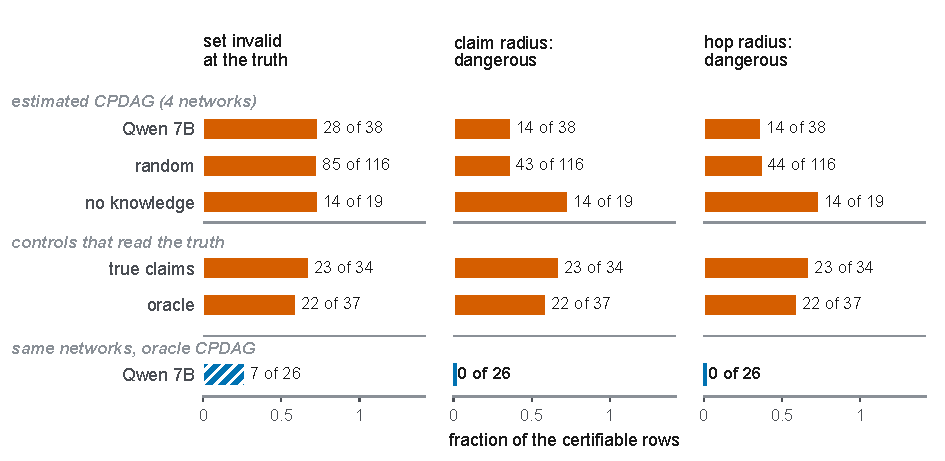
\includegraphics[width=0.9\linewidth]{pest_dangerous.pdf}
\caption{On the learned CPDAG the claim radius and the hop radius are dangerous on the same rows, and
truthful claims do not rescue them. On the oracle CPDAG of the same four networks the supplier's two
radii
are dangerous on none of its 26 rows. The error that breaks the set is in the learned graph, where no
retraction of
claims reaches it.}
\label{fig:pest}
\end{figure}

\figref{fig:pest} sets the two panels side by side. Without knowledge there is no claim to retract,
the certificate reports no break, and every invalid set becomes dangerous. The truthful condition
asserts nothing false and is still dangerous on 23 of 34 rows,
because the error is in the graph. In the ledger the two radii differed by the unit; here both reason
inside the wrong class
and certify the same broken sets, and over the whole panel they differ on one row.

The certifiable share rose instead of falling, which falsified P2: the primary supplier certifies 38 of
80 frame rows (0.475) against 26 of 80 (0.325) on the oracle panel. The learned graph orients more than
the truth does, and identifiability is bought with wrong orientations. \texttt{magic-niab}, whose
reference misses no skeleton edge and adds one, is the only network where neither the supplier nor
chance is ever dangerous, and all their invalid sets (6 and 14) are detected. The audit conditions are
still dangerous there on 3 and 4 rows, because 14 of its 62 compelled edges point the wrong way.

\prompt[conceito=premissa-classe,dificuldade=0.8]{\texttt{magic-niab} is the one network with no
dangerous row on the deployment conditions. Why does that confirm the scope limit rather than weaken
it, and why are the audit conditions still dangerous there?}{Its reference skeleton misses no edge
and adds one, so the invalid sets of the supplier and of chance come from their claims, which the
certificate sees: all 6 and 14 are detected. The truth still does not extend the analyst's graph,
because 14 of 62 compelled edges are wrong, and the audit conditions, which assert only true claims,
are dangerous on 3 and 4 rows: an error on a compelled edge that no retraction reaches. The limit shows
up exactly where the premise almost holds.}

% -----------------------------------------------------------------------------
\begin{antes}
\antesq[premissa-classe]{Name the three mechanisms the inspection found on the dangerous rows of the
supplier and of no knowledge.}
\antesq[correcao-minima]{Why can no retraction of claims repair an edge the data got wrong?}
\end{antes}

\section{Why no retraction reaches the error}\label{sec:pest-why}

P3 carried the ledger's decision rule, and it fired: the six dangerous rows of the supplier and of no
knowledge that passed its test (three queries, two networks) were inspected before anything else was
read. No bug: each committed set is valid on the analyst's graph and contains
a node the truth forbids.

\begin{exemplo}[A true claim, a dangerous row]\label{ex:pest-collider}
The data suggest a collider that does not exist: the learned CPDAG compels $X \to Y \leftarrow H$ and
leaves $W - X$ open. The analyst asserts $W \to X$, which is true.

\begin{center}
\begin{tikzpicture}[x=1cm, y=1cm]
\begin{scope}
\node[font=\scriptsize\sffamily] at (2.25,0.8) {analyst's graph $\Gz$: learned class + one true claim};
\node[nodo] (w) at (0,0) {$W$};
\node[nodo] (x) at (1.5,0) {$X$};
\node[nodo] (y) at (3.0,0) {$Y$};
\node[nodo, draw=verdesc, very thick] (h) at (4.5,0) {$H$};
\draw[afirmada] (w) -- (x);
\draw[aresta] (x) -- (y);
\draw[falsa] (h) -- (y);
\node[font=\scriptsize\sffamily, text=verdesc] at (4.5,-0.6) {$Z = \{H\}$};
\node[font=\tiny\sffamily, text=vermesc] at (3.75,0.3) {wrong};
\end{scope}
\begin{scope}[xshift=7.4cm]
\node[font=\scriptsize\sffamily] at (2.25,0.8) {the truth};
\node[nodo] (w) at (0,0) {$W$};
\node[nodo] (x) at (1.5,0) {$X$};
\node[nodo] (y) at (3.0,0) {$Y$};
\node[nodo, draw=vermesc, very thick] (h) at (4.5,0) {$H$};
\draw[aresta] (w) -- (x);
\draw[aresta] (x) -- (y);
\draw[aresta] (y) -- (h);
\node[font=\scriptsize\sffamily, text=vermesc] at (4.5,-0.6) {child of $Y$};
\end{scope}
\end{tikzpicture}
\end{center}

On $\Gz$ the optimal set for $X \to Y$ is $\mathrm{pa}(Y) \setminus \{X\} = \{H\}$, and it is valid.
Retracting $W \to X$ reopens $W - X$ and leaves $H \to Y$ alone, since no claim created it, so $\{H\}$
stays valid and the certificate reports no break. At the truth $H$ is a child of $Y$, hence forbidden,
and $\{H\}$ is invalid. The row is dangerous with no false claim at all.
\end{exemplo}

The measured rows follow the same pattern with real variables. On \texttt{magic-irri}, for the effect
on \texttt{FT}, $\Chat_E$ compels \texttt{HT} $\to$ \texttt{FT} and \texttt{YLD} $\to$ \texttt{FT}
against the truth, so both variables, descendants of the outcome in the truth, enter the set; that is
the example above. The other two mechanisms are missing edges: on \texttt{magic-irri}, for the effect
of \texttt{GTEMP}, $\Chat_E$ lacks \texttt{GTEMP} -- \texttt{GW}, so \texttt{GW}, which the truth
forbids, enters the set; on \texttt{arth150}, $\Chat_E$ lacks three of the treatment's edges and 11
members of the set are forbidden at the truth (\texttt{PREREGISTRATION.md}, A.1, P3).

The inspection also showed that P3 had been registered on the wrong test: it looked only at the claims
and the query, and an error in the skeleton or in a compelled edge passes it. The exact test,
\texttt{truth\_extends\_g0}, was added after the first table and is marked post hoc; the frozen
instrument rows were byte-identical across both runs. Written with its premise in view,
Proposition~\ref{prop:t4-structural} says: \emph{if the true DAG belongs to the class of $\Chat$},
retracting the false claims lands on a graph the truth extends. Without that clause nothing follows,
and on this panel the clause held on no row.

\prompt[conceito=premissa-classe,dificuldade=0.75]{State the structural property of the claim radius
with the premise P-EST removed, and say on how many certifiable rows of the panel the premise
held.}{With certificate and audit on the same criterion, and supposing the true DAG belongs to the
class of $\Chat$: if the committed set is invalid at the truth and $w$ claims are false, retracting
those $w$ claims leaves a graph the truth extends, where the set fails, so $\rclaim \le w$ and the
claim radius does not over-certify. The premise is that the class contains the truth. On the panel it
held on 0 of 244 certifiable rows.}

% -----------------------------------------------------------------------------
\begin{antes}
\antesq[pre-registro]{Which of P1 to P5 turned out vacuous, and why?}
\antesq[frases-proibidas]{What is the licensed sentence for this panel, and which sentence does it
forbid?}
\end{antes}

\section{Predictions, and the sentence the paper can print}

\begin{center}\footnotesize
\begin{tabular}{@{}l>{\raggedright\arraybackslash}p{4.4cm}>{\raggedright\arraybackslash}p{3.1cm}>{\raggedright\arraybackslash}p{6.0cm}@{}}
\toprule
& \textbf{prediction} & \textbf{verdict} & \textbf{what decided it} \\
\midrule
P1 & estimation leaves more open than the oracle, less as $n$ grows & not supported as registered &
holds for PC (non-increasing on three networks); GES at $n = 200$ is sparse and almost fully oriented \\
P2 & the certifiable share falls & falsified & 0.475 against 0.325 \\
P3 & no dangerous row where the truth extends the graph & falsified as operationalised; premise held
on no row & truth extends $\Gz$ on 0 of 244; the inspection found no bug \\
P4 & wrong-skeleton rows are counted, not dropped & partly supported & nothing dropped; one of the two
statuses never fires \\
P5 & realised bias larger at certified floor 1 & supported as registered, not robust & 0.110 against
0.063; medians reverse \\
\bottomrule
\end{tabular}
\end{center}

P5 is supported only as pooled means (absolute bias of the OLS estimate 0.110 on 71 rows at floor 1,
0.063 on 102 at floor 2 or more, deployment conditions): the medians reverse, and so do the means
without \texttt{magic-irri}. On an invalid set the bias is structural, so the certified floor is not a
bias proxy on this panel.

\begin{sonorio}[The licensed form, \texttt{docs/PROTOCOL\_RUN.md}, stage 6]
\emph{The claim radius certifies against error in the analyst's claims given a correct equivalence
class. It does not certify against discovery error, which on these four networks at $n = 5000$
invalidates more committed sets than the claims do.} It goes in the main text (one results paragraph,
one sentence in the limitations, Table~7 in the appendix), as \texttt{results/pest/PREREGISTRATION.md}
A.2 says. Never «robust under an estimated
CPDAG», for the claim radius or for the hop radius.
\end{sonorio}

The wrong use of this panel is the usual limitations sentence, and your draft has one.

\begin{armadilha}[A scope limit, not a softened idealisation]
Section~7 of your draft says: «The skeleton and the v-structures are treated as given \ldots\ Real
discovery on finite data returns a different and usually sparser skeleton, and a missing weak edge is
precisely the error that breaks back-door blocking; nothing here speaks to it.» The mechanism is right,
and it is one of the two the inspection found; the other is a compelled edge pointing the wrong way.
«Nothing here speaks to it» is no longer true: P-EST measured that the guarantee fails, not an
idealisation to relax later. A deployment claim for either radius needs a certificate that also
retracts the discovery output; the panel sizes that gap and does not close it.
\end{armadilha}

\prompt[conceito=pre-registro,dificuldade=0.7]{P5 came out supported as registered: mean bias 0.110
at certified floor 1 against 0.063 at floor 2 or more. Give the three readings that stop anyone calling
the floor a bias proxy.}{The medians reverse, 0.021 against 0.028. Without \texttt{magic-irri} the
means reverse too, 0.047 against 0.050, because the pooled order comes from that network's 14 chance
rows at floor 1, averaging 0.344. And of the eight network-by-condition cells with rows at both floors,
four go each way. On an invalid set the bias is structural anyway, and a sampling band says nothing
about it.}

% -----------------------------------------------------------------------------
\begin{antes}
\antesq[var-sortability]{How close to one are var-sortability and $R^2$-sortability on the four
Gaussian networks?}
\antesq[invariante]{What exactly is the \texttt{sachs} network in the repository, and what word must
the paper never use for it?}
\end{antes}

\section{The substrate decisions behind Table 2}

Table~2 describes the corpus network by network (\texttt{results/substrate/TABLE2\_SUBSTRATE.md}).
Four decisions were closed on 12 September in \texttt{results/substrate/DECISIONS.md}, and the first
concerns the four networks of this chapter.

\begin{medido}[Sortability, \texttt{results/substrate/sortability.json}]
\texttt{experiments/sortability\_probe.py}, $n = 5000$, ten seeds, definitions of Reisach et al.\
(2021, 2023) implemented from the papers.
Var-sortability 0.62 (\texttt{arth150}), 0.71 (\texttt{ecoli70}), 0.59 (\texttt{magic-irri}), 0.33
(\texttt{magic-niab}); $R^2$-sortability 0.25, 0.38, 0.61, 0.76. Seed dispersion at most 0.015; every
mean within about one standard deviation of its population value.
\end{medido}

None of the four sits near one on either criterion, and the two do not track each other
(\texttt{arth150} has the second-highest var-sortability and the lowest $R^2$-sortability). A learned
CPDAG on these networks cannot be read off the variances, so the discovery errors of P-EST
are not an artefact of an easy ordering; every other network is undefined, having no continuous
parameters.

The other three decisions fix what three files are. \texttt{M-bias.txt}, dagitty's three-node ADMG, is
refused as a DAG and expanded into \texttt{M-structure.txt}, five nodes with both latent causes
explicit; once they are measured the trap disappears (the optimal set for $(E, D)$ is $\{U_2\}$ either
way), so it is a calibration fixture outside the frozen frame and the ledger. In
\texttt{Didelez\_2010} the node \texttt{S} is dagitty's \texttt{selected} indicator; it
changes no orientation, and the 48 ledger rows with \texttt{S} as outcome are declared as a named
stratum. \texttt{sachs} is byte-identical to bnlearn's file: the 17-arc network that Sachs et
al.\ (2005) inferred, which differs from the 20-edge Tetrad ground truth by one reversal
(\texttt{Plcg}--\texttt{PIP3}) and three added edges. Its CPDAG is fully undirected, and on that one
edge five knowledge
conditions answered in the map's direction and two in the file's. The commission count on
\texttt{sachs} depends on the choice, and the paper names the object and never calls it the consensus
network.

\prompt[conceito=invariante,dificuldade=0.7]{What is \texttt{sachs} in the repository, how does it
differ from the Tetrad ground truth, and why does the difference change a measured
number?}{bnlearn's 17-arc network inferred in Sachs et al.\ (2005), with tables fitted to discretised
data. The Tetrad ground truth has 20 edges: it shares 16, reverses \texttt{Plcg}--\texttt{PIP3} and
adds three. The CPDAG of the 17-arc graph is fully undirected, so the reversed edge is a claim; five
conditions answered \texttt{PIP3} $\to$ \texttt{Plcg} and two \texttt{Plcg} $\to$ \texttt{PIP3}, so
which group is scored as wrong depends on which object is called the truth.}

\naopasse[premissa-classe]{In Example~\ref{ex:pest-collider}, point to the edge that makes the row
dangerous and say why retracting $W \to X$ cannot reach it. If you pointed to the claim $W \to X$,
reread the example before the exercises.}

\begin{exercicio}[metodo=counterexample,conceito=premissa-classe]
P3 was registered on rows whose claims all name true edges in the true direction and whose outcome is
a true descendant of the treatment. A colleague argues that on such rows the claim radius cannot be
dangerous, since every claim is true. Refute it with four nodes, using a \emph{missing} edge rather
than the wrong collider of Example~\ref{ex:pest-collider}: give the truth, the learned CPDAG, the claim,
the committed set, and the bucket. Which measured mechanism does your construction reproduce?
\end{exercicio}
\begin{solucao}
Truth: $W \to X$, $X \to Y$, $X \to C$, $C \to Y$, so $C$ is a mediator. The learned skeleton misses
$X - C$; with $X$ and $C$ non-adjacent, $X \to Y \leftarrow C$ is compelled as a v-structure and $W - X$
stays open. The analyst asserts $W \to X$, which is true, and $Y$ is a true descendant of $X$, so the
row passes P3's test. On $\Gz$ the optimal set is $\mathrm{pa}(Y) \setminus \{X\} = \{C\}$, valid
because $C$ is not a descendant of $X$ there. Retracting $W \to X$ leaves $\{C\}$ valid, so the
certificate reports no break and covers $w = 0$. At the truth $C$ lies on the causal path
$X \to C \to Y$, is forbidden, and $\{C\}$ is invalid: dangerous. It reproduces the missing-edge
mechanism of
\texttt{GTEMP} -- \texttt{GW} on \texttt{magic-irri}; Table~7 counts 3 rows of the supplier that pass
P3's test and are dangerous.
\end{solucao}

\begin{exercicio}[metodo=rewriting,conceito=frases-proibidas]
Rewrite the first two sentences of the paragraph quoted in the trap of this chapter («Assumptions
inherited by every number», Section~7 of your draft) so that they carry what P-EST measured, in at most
five sentences, in the paper's register: no percentages in parentheses on every clause, no forbidden
phrase, and the premise stated as the scope of the certificate.
\end{exercicio}
\begin{solucao}
One acceptable version: \emph{The radius certifies against error in the analyst's claims given a
correct equivalence class; the skeleton and the v-structures are treated as given. We measured what
happens when that condition is dropped. On four networks with fitted Gaussian parameters we learned the
class with PC from 5,000 samples and rebuilt every stage on it: no learned class contained the true
graph, and the committed set was invalid at the truth on 28 of the 38 certifiable queries of the
primary knowledge source. Both the claim radius and the hop radius over-certified on 14 of them, and
truthful claims did not prevent it, because a missing edge or a wrong compelled orientation lies
outside every retraction of claims.} What changed: the premise became the scope of the
certificate, «nothing here speaks to it» became a measurement, and «usually sparser» went, since the
learned classes both lose and add edges and orient more than the truth.
\end{solucao}

\section*{Chapter map}

\begin{center}
\begin{tikzpicture}[x=1cm, y=1cm, lb/.style={font=\tiny\sffamily, align=center}]
\node[cmapc] (g)  at ( 0.0, 0)    {claim radius's guarantee};
\node[cmap]  (p)  at (-4.4, 0)    {premise: the class contains the truth};
\node[cmapg] (o)  at ( 4.4, 0)    {oracle panel: dangerous on 0 rows};
\node[cmap]  (a)  at (-4.4,-1.45)  {learned CPDAG: PC and GES, three $n$, ten seeds};
\node[cmapr] (e)  at ( 0.0,-1.45)  {truth extends $\Gz$ on 0 of 244};
\node[cmapr] (d)  at ( 4.4,-1.45)  {dangerous on 14 of 38; hop radius the same 14};
\node[cmap]  (n)  at (-2.2,-2.8)  {missing edges, wrong compelled edges};
\node[cmapg] (s)  at ( 2.2,-2.8)  {licensed: given a correct class};
\draw[cedge] (p) -- node[lb, above]{sustains} (g);
\draw[cedge] (g) -- node[lb, above]{holds on} (o);
\draw[cedge] (p) -- node[lb, left]{tested by} (a);
\draw[cedge] (a) -- node[lb, above]{voids} (e);
\draw[cedge] (e) -- node[lb, above]{so} (d);
\draw[cedge] (n) -- node[lb, left, pos=0.4]{no retraction\\ reaches} (e);
\draw[cedge] (d) -- node[lb, right, pos=0.4]{scopes\\ the claim} (s);
\end{tikzpicture}
\end{center}


\part{Pricing knowledge: the Rosenbaum analogue}
% =============================================================================
\chapter{Rosenbaum's \texorpdfstring{$\Gamma$}{Gamma}, and Table 1 on real structure (M1)}\label{ch:gamma}

Chapters~\ref{ch:frame} to~\ref{ch:pest} audited a certificate. This chapter is about what the
paper is for, and about the first measurement that answers that question on real structures.

\begin{ideia}[The paper in two sentences]
Rosenbaum did not test what the data cannot test: he asked how strong hidden confounding would
have to be to overturn the conclusion. We ask the same question of background knowledge, and the
unit of violation is the number of the analyst's orientation claims that would have to be withdrawn.
\end{ideia}

\begin{antes}
\antesq[deriva-enquadramento]{The first measurement-paper draft of 12 September had correct
numbers. What was wrong with it?}
\antesq[gamma-de-rosenbaum]{What does $\Gamma$ bound, in what design, and what does $\Gamma = 1$
mean?}
\end{antes}

\section{12 September: the subject was wrong}

On 12 September, with Table~4 of the ledger just out, I wrote a full draft of the measurement paper,
\emph{Claim Radius: Certifying Covariate Adjustment Sets Against Misspecified Background Knowledge}.
Its numbers came from the result files, and its centre was the supplier ledger: knowledge suppliers
from 7B to 72B, scrambled names, a scale axis as a table of its own. That was the wrong paper. The
evaluation protocol had been built first, and its most elaborate arm had become the subject. What we
set out to write is an uncertainty measure for background knowledge, the analogue of Rosenbaum's
$\Gamma$ for orientation claims. Elicited knowledge is one of four knowledge processes in the
evaluation (with controlled reversals, chance orientations and truthful controls, the last asserting nothing false), never the title,
the abstract's lead or Table~1. Your related-work paragraph (\texttt{sections/03\_related\_work.tex})
already has the sentence: the radius asks the structural analogue of how strong a confounder must be.
The change is that this sentence becomes the spine of the paper.

\textbf{What Rosenbaum does.} In a matched study each pair joins a treated and a control unit with
the same observed covariates; with perfect matching either member is equally likely to be the treated
one. An unmeasured covariate breaks this. Rosenbaum does not estimate it: he lets the two members
differ in their odds of treatment by at most a factor $\Gamma$, redoes the inference in the worst case
the model allows, and reports the $\Gamma$ at which the conclusion is lost.

\begin{exemplo}[Illustrative: the numbers are constructed for this page, not measured in any study]
Take 40 discordant pairs with a binary outcome; in each, exactly one member had the event, and in
30 of them it was the treated one. With no treatment effect and $\Gamma = 1$, the count $T$ of
pairs where the treated member had the event is $\mathrm{Bin}(40, 1/2)$ and the one-sided p-value is
$P(T \ge 30) \approx 0.001$. With $\Gamma > 1$ the chance that the event member is the treated one
may be as large as $p^{+} = \Gamma/(1+\Gamma)$, and the worst-case p-value is the upper tail of
$\mathrm{Bin}(40, p^{+})$. For $\Gamma = 1, 1.25, 1.5, 1.6, 1.75$ it is $0.001, 0.009, 0.035, 0.053,
0.089$ (exact binomial tails, computed for this page). Significance at 5\,\% is lost near
$\Gamma^{*} \approx 1.58$, and the report reads: the conclusion survives a hidden confounder that
multiplies the within-pair odds of treatment by up to 1.58, and falls above that.
\end{exemplo}

The example is the sign test, the simplest case of this model.

\begin{definicao}[Sensitivity model and sensitivity value]
Let $\pi_{1}, \pi_{2}$ be the treatment probabilities of two members of a pair with the same observed
covariates. The model with parameter $\Gamma \ge 1$ admits every assignment with
\[
\frac{1}{\Gamma} \;\le\; \frac{\pi_{1}(1-\pi_{2})}{\pi_{2}(1-\pi_{1})} \;\le\; \Gamma .
\]
Given that exactly one member is treated, the probability that it is the first lies in
$[1/(1+\Gamma),\ \Gamma/(1+\Gamma)]$, and $\Gamma = 1$ is randomisation within the pair. The
\emph{sensitivity value} $\Gamma^{*}$ is the smallest $\Gamma$ at which the worst-case p-value over
the model exceeds the level $\alpha$.
\end{definicao}

\prompt[conceito=gamma-de-rosenbaum,dificuldade=0.7]{State what $\Gamma$ bounds, why $\Gamma = 1$ is
the randomised experiment within pairs, and why the worst-case p-value can only grow with
$\Gamma$.}{$\Gamma$ bounds the ratio of the odds of treatment of two members of a pair that agree on
the observed covariates: a hidden confounder can tilt that chance by at most this factor. At
$\Gamma = 1$ both members have the same chance, which is a coin flip within the pair. The worst-case
p-value is a maximum over the admitted assignments, and the set admitted at $\Gamma'$ contains the
set admitted at any $\Gamma < \Gamma'$; a maximum over a larger set cannot decrease. So there is a
single point where significance is lost, $\Gamma^{*}$.}

\begin{antes}
\antesq[intervalo-conhecimento]{Which object of ours plays the worst-case p-value at each $\Gamma$,
and which plays $\Gamma^{*}$?}
\antesq[rval]{Which of our two radii has no counterpart in Rosenbaum?}
\end{antes}

\section{The translation, and where it breaks}

Inside a Markov equivalence class every graph generates the same observational distributions, and
Meek's rules certify that claims are consistent, not true: no test on the data separates an
orientation from its reverse. That is the position of Rosenbaum's unmeasured covariate, and it takes
the same answer, price the error instead of measuring it. The red rows are where the analogy breaks.

\begin{center}
\begin{tikzpicture}[
  lbox/.style={draw=laranjaesc, fill=laranjaesc!7, rounded corners=2pt, text width=5.2cm,
               minimum height=0.78cm, align=left, font=\scriptsize, inner sep=2.5pt},
  rbox/.style={draw=azulesc, fill=azulesc!6, rounded corners=2pt, text width=5.2cm,
               minimum height=0.78cm, align=left, font=\scriptsize, inner sep=2.5pt},
  xbox/.style={draw=vermesc, fill=vermesc!6, rounded corners=2pt, text width=5.2cm,
               minimum height=0.78cm, align=left, font=\scriptsize, inner sep=2.5pt},
  vbox/.style={draw=cinzamedio, dashed, rounded corners=2pt, text width=5.2cm,
               minimum height=0.78cm, align=center, font=\scriptsize, text=cinzamedio, inner sep=2.5pt},
  mid/.style={font=\scriptsize\sffamily\bfseries, text width=2.6cm, align=center, text=cinzaescuro},
  midx/.style={font=\scriptsize\sffamily\bfseries, text width=2.6cm, align=center, text=vermesc},
  y=0.81cm]
\node[font=\small\sffamily\bfseries, text=laranjaesc] at (-4.5,0.75) {Rosenbaum: matched pairs};
\node[font=\small\sffamily\bfseries, text=azulesc] at (4.5,0.75) {Our paper: orientation claims};
\foreach \yy/\mtxt/\ltxt/\rtxt/\rst/\mst in {
  0/{what the data\\ cannot test}/{an unmeasured covariate $u$ within pairs equal on the observed
     $x$}/{the orientations in $\Kset$ inside the class: Meek checks consistency, not
     truth}/rbox/mid,
  -1/{the parameter}/{$\Gamma \ge 1$: within-pair odds ratio of treatment}/{$r = 0,1,2,\dots$:
     the number of the analyst's claims allowed to be wrong}/rbox/mid,
  -2/{the report at\\ each value}/{the worst-case p-value over the assignments $\Gamma$
     admits}/{$\Ir{r}$: hull of the 95\,\% bands of the effects over the graphs of
     $\Ball{r}$}/rbox/mid,
  -3/{the breakdown\\ value}/{$\Gamma^{*}$: smallest $\Gamma$ at which significance is
     lost}/{$\rnul$: smallest $r$ at which the band contains zero}/rbox/mid,
  -4/{the scale}/{continuous: $\Gamma^{*} \approx 1.58$ is an ordinary report}/{an integer; on real
     structures $\rnul$ is almost always 1 or beyond 3}/xbox/midx,
  -5/{the reading}/{a parameter of a model for treatment assignment}/{a count with no probability
     reading: it does not estimate how many claims are wrong}/xbox/midx}
{
  \node[lbox] (L) at (-4.5,\yy) {\ltxt};
  \node[\mst] (M) at (0,\yy) {\mtxt};
  \node[\rst] (R) at (4.5,\yy) {\rtxt};
  \draw[-{Stealth[length=1.4mm]}, cinzamedio] (L.east) -- (M.west);
  \draw[-{Stealth[length=1.4mm]}, cinzamedio] (M.east) -- (R.west);
}
\node[vbox] at (-4.5,-6.15) {no counterpart};
\node[mid] at (0,-6.15) {a second radius};
\node[rbox] at (4.5,-6.15) {$\rval$: smallest $r$ at which the committed set $Z$ stops being
     valid};
\end{tikzpicture}
\end{center}

In symbols, with $\Gz = \mathrm{Meek}(\Chat, \Kset)$ and the committed set $Z = \Ostar(\Gz)$ read off
the analyst's graph, the right-hand column is this.

\begin{formulabox}[The translation, formally]
\[
\Ball{r} = \bigl\{\mathrm{Meek}(\Chat, \Kset \setminus S) : S \subseteq \Kset,\ |S| \le r\bigr\},
\qquad
\Ir{r} = \operatorname{hull} \bigcup_{G \in \Ball{r}} \mathrm{band}_{95}(G),
\]
\[
\rnul = \min\{r : 0 \in \Ir{r}\}, \qquad
\rval = \min\{r : Z \text{ is not valid in some } G \in \Ball{r}\},
\]
and each endpoint of $\Ir{r}$ comes with the set $S$ that produces it, named in the domain's
variables. Both events are upward closed in $r$ because $\Ball{r} \subseteq \Ball{r+1}$.
\end{formulabox}

A real analysis shows the translation end to end. The query G311 $\to$ G43 on \emph{magic-niab},
whose coefficients are fitted to real measurements, has two claims in the treatment's chain
component under the larger supplier's knowledge, and both are true.

\begin{medido}[One report, \texttt{results/interval/fig1\_candidates.json}, relaxed list (outside the registered rule), row 1]
True effect $-0.255$; estimate $-0.251$ $[-0.259, -0.244]$ at $n = 20\,000$. The band barely moves at
$r = 1$ (width ratio 1.06) and reaches zero at $r = 2$, when G1853 $\to$ G311 and G311 $\to$ G43 are
both retracted: $\rnul = 2$ on 20 of 20 seeds, $\rval = 2$. The supplier made six claims in the
network, three false, all outside the component.
\end{medido}

Read as Rosenbaum would: the conclusion that G311 lowers G43 rests on two named claims and survives the
withdrawal of either. Three breaks in the analogy have to be said once, in the paper. The scale is an
integer and, on real structures, almost without a middle (next section). There is no probability model
behind $r$: this row has $\rnul = 2$ with both local claims true and three false claims elsewhere, so
$r$ counts claims whose withdrawal changes the conclusion, not claims that are wrong. And the report is
honest only if the class contains the truth, which fails once the CPDAG is estimated
(Chapter~\ref{ch:pest}).

\prompt[conceito=intervalo-conhecimento,dificuldade=0.65]{Complete the translation: $\Gamma$
becomes what, the worst-case p-value becomes what, $\Gamma^{*}$ becomes what, and which object of
ours has no counterpart in Rosenbaum?}{$\Gamma$ becomes $r$, the number of the analyst's claims
allowed to be wrong. The worst-case p-value becomes the knowledge interval $\Ir{r}$, the hull of the
95\,\% bands over the graphs of the retraction ball $\Ball{r}$. $\Gamma^{*}$ becomes the null radius
$\rnul$, the smallest $r$ at which the band contains zero. The validity radius $\rval$ has no
counterpart: a matched design does not read an adjustment set off a graph that can break. The named
witnesses of each endpoint are also ours.}

\begin{antes}
\antesq[linhas-procedimento]{What do the rows of Table~1 have in common, and what do they differ
in?}
\antesq[colunas-cruzamento]{With one wrong claim, how much does the stated report cover, and at what
width does the one-claim interval restore coverage?}
\antesq[metrica-unica]{What does an $\Lnf$ above 1 mean?}
\end{antes}

\section{M1: Table 1 on real structure}

Before M1 the headline table existed only on synthetic generators, uncalibrated. Its
pre-registration (\texttt{results/interval/PREREGISTRATION.md}, P1 to P9) was written on 12 September
before \texttt{experiments/interval\_panel.py} produced a row. A run takes about 90 seconds; five runs
with 3 to 7 processes gave a byte-identical \texttt{rows.csv}.

\textbf{Design.} The frozen frame, 528 queries. Panel~A: the 23 other networks of the ledger, real
structure, semi-synthetic coefficients (magnitude uniform on $[0.5, 1.5]$, random sign, unit noise),
448 queries. Panel~B: \texttt{ecoli70}, \texttt{arth150}, \texttt{magic-niab}, \texttt{magic-irri}
with fitted coefficients, 80 queries. Knowledge: controlled reversals of $b = 0, 1, 2$ true claims
inside the treatment's chain component (a reversal outside it moves no interval, a reduction tested
against brute force on 7,770 pairs), and the 7B and 72B suppliers' elicited claims stratified by false
local claims. Samples at $n = 1000$ and $20\,000$, twenty seeds. \textbf{One estimator} in every row,
the OLS coefficient of $X$ given a set; rows differ only in the graphs the hull is taken over: the
committed report (PLAIN), a matched control retracting one claim far from $X$ and $Y$ (FAR1),
$\Ir{1}$, $\Ir{2}$, and the whole class (BLANKET, discarding the knowledge). The metric $\Lnf$
stretches each procedure's intervals by the smallest common factor giving 95\,\% coverage in the cell
and divides the mean stretched width by BLANKET's (Chapter~\ref{ch:tables} opens a cell).
\textbf{Above 1 means wider than throwing the knowledge away.}

\begin{table}[!ht]
\centering\footnotesize
\setlength{\tabcolsep}{3.4pt}
\caption{M1, informative queries, $n = 1000$: $\Lnf$ [network-bootstrap 95\,\% interval] / raw
coverage. The three columns are different populations (see the rows line). Source:
\texttt{results/interval/TABLE1\_L95.md}.}
\label{tab:m1-gamma}
\begin{tabular}{@{}l ll ll ll@{}}
\toprule
 & \multicolumn{2}{c}{$b = 0$} & \multicolumn{2}{c}{$b = 1$} & \multicolumn{2}{c}{$b = 2$} \\
\cmidrule(lr){2-3}\cmidrule(lr){4-5}\cmidrule(lr){6-7}
procedure & $\Lnf$ & cov. & $\Lnf$ & cov. & $\Lnf$ & cov. \\
\midrule
\multicolumn{7}{@{}l}{\emph{Panel~A, semi-synthetic coefficients, 23 networks}} \\
PLAIN (committed) & 0.464 [0.35, 0.57] & 0.967 & 5.123 [3.24, inf) & 0.597 & 4.082 [2.71, inf) & 0.554 \\
FAR1 (control)   & 0.655 & 0.967 & 10.771 & 0.640 & 7.539 & 0.614 \\
$\Ir{1}$         & 0.957 [0.87, 0.99] & 0.982 & 0.851 [0.76, 0.94] & 0.980 & 4.234 & 0.781 \\
$\Ir{2}$         & 0.984 & 0.984 & 0.980 & 0.984 & 0.847 [0.74, 0.94] & 0.984 \\
BLANKET (class)  & 1.000 & 0.984 & 1.000 & 0.985 & 1.000 & 0.988 \\
rows (networks)  & 391 (23) & & 359 (23) & & 131 (9) & \\
\midrule
\multicolumn{7}{@{}l}{\emph{Panel~B, fitted coefficients, 4 networks}} \\
PLAIN            & 0.840 [0.76, 0.88] & 0.969 & 3.316 [0.81, 4.59] & 0.885 & 2.588 & 0.891 \\
$\Ir{1}$         & 0.979 & 0.979 & 0.974 [0.94, 1.00] & 0.980 & 0.887 & 0.947 \\
$\Ir{2}$         & 0.997 & 0.980 & 0.989 & 0.983 & 0.945 & 0.979 \\
rows (networks)  & 69 (4) & & 44 (4) & & 35 (4) & \\
\bottomrule
\end{tabular}
\end{table}

On Panel~A, with no wrong claim the committed report is the narrowest (0.464) and the one-claim
interval pays a premium (0.957): insurance costs when nothing is wrong (P1). With one wrong claim the
committed report covers 0.597 and would need 5.1 class widths to reach 95\,\%, while $\Ir{1}$ covers
0.980 at 0.851 of the class width. With two, $\Ir{1}$ is not enough (0.781) and $\Ir{2}$ pays.
\figref{fig:l95} draws the crossing.

\begin{figure}[!ht]
\centering
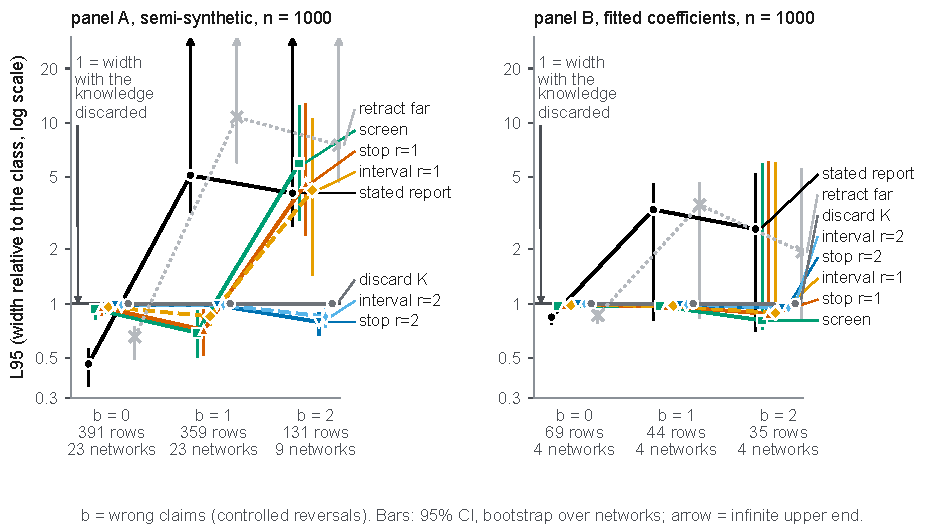
\includegraphics[width=0.74\linewidth]{l95_crossing.pdf}
\caption{Panel~A: with one wrong claim the committed report costs more than five class widths and
retracting a far claim does not help; with two, only the budget-two procedures stay below 1. Panel~B's
four networks keep the order at smaller magnitudes. The columns are different populations, so the lines
between them do not follow the same analyses.}
\label{fig:l95}
\end{figure}

\begin{medido}[The crossing and the saving, \texttt{results/interval/TABLE1\_L95.md} and \texttt{PREREGISTRATION.md} A.2]
Against discarding the knowledge, $\Ir{1}$ at $b = 1$ saves 14.9\,\% of the width at $n = 1000$ and
24.2\,\% at $n = 20\,000$ on Panel~A (0.851 and 0.758), and 2.6\,\% and 4.8\,\% on Panel~B (0.974 and
0.952). With errors nobody planted (elicited, one false local claim, suppliers pooled, $n = 1000$)
the order repeats: PLAIN 0.600 at $\Lnf$ 6.92 against 0.867 for $\Ir{1}$ on Panel~A (208 rows), 0.696
at 2.41 against 0.901 on Panel~B (23 rows). P1, P2, P4, P5, P7, P8, P9 supported; P3 partial; P6
falsified.
\end{medido}

The saving is modest, and the paper should say so: the interval covers where the committed report does
not, at less than the price of discarding the knowledge.

\prompt[conceito=colunas-cruzamento,dificuldade=0.75]{Panel~A, $n = 1000$, one wrong claim: give the
coverage and $\Lnf$ of the committed report and of $\Ir{1}$, and say what 5.12 means.}{PLAIN covers
0.597 with $\Lnf = 5.123$; $\Ir{1}$ covers 0.980 with $\Lnf = 0.851$ [0.76, 0.94], over 359
informative queries on 23 networks. The 5.12 means that to reach 95\,\% coverage the committed
report's intervals would have to be stretched to a mean width of 5.1 times the calibrated width of the
whole class: trusting one wrong claim costs more than discarding all the knowledge.}

\begin{antes}
\antesq[r0-binario]{Where an effect is established with the full knowledge, what values does
$\rnul$ take on real structures?}
\antesq[banda-plugin]{How often does the hull of point estimates state a null radius above the
population one, and how often does the band?}
\end{antes}

\section{What M1 changed in the report}

The translation promises a scale: how many wrong claims until the conclusion falls. On real
structures the scale has almost no middle.

\begin{medido}[$\rnul$ by knowledge condition, counted in \texttt{results/interval/rows.csv} (\texttt{r0\_pop})]
Frame queries with an effect established under the full knowledge ($\rnul \ge 1$); ``beyond 3''
pools \texttt{>3}, \texttt{never} and censored. Panel~A, true claims ($b = 0$): 221 queries, $\rnul = 1$
on 71, 2 or 3 on 16, beyond 3 on 134, so 1 or beyond 3 on 92.8\,\%. The same share is 88.8\,\% at
$b = 1$, 74.2\,\% at $b = 2$ (66 queries), 93.6\,\% (7B), 94.1\,\% (72B) and 97.7\,\% under the
recovering set (6 of 257 at 2 or 3). Panel~B: 25 of 25 at $b = 0$, 33 of 38 under 72B. Restricted to
informative queries the $b = 0$ share on Panel~A is 148 of 164 (90.2\,\%): a non-informative query
with a nonzero effect is ``never'' by construction.
\end{medido}

\begin{figure}[!ht]
\centering
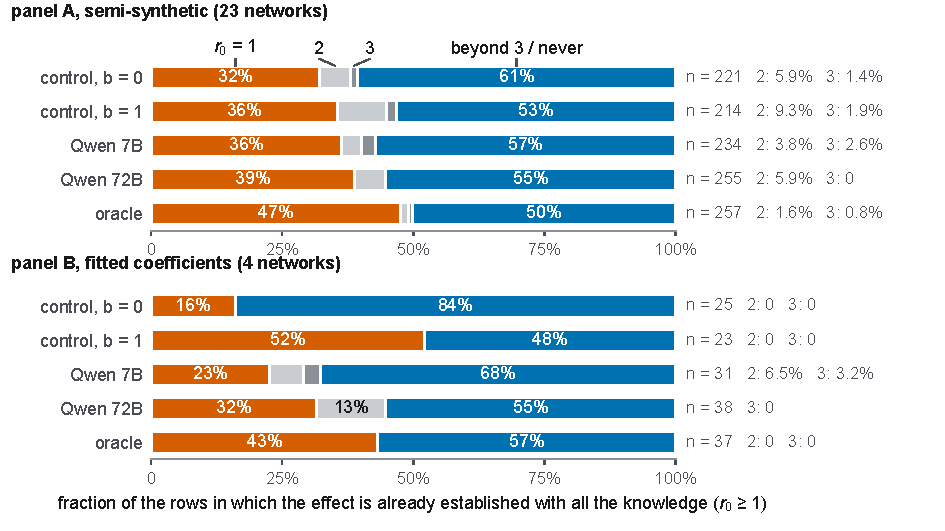
\includegraphics[width=0.70\linewidth]{r0_distribution.pdf}
\caption{Under every knowledge source and on both panels, where an effect is established the
conclusion rests on one claim or on none within depth three: the mass at 2 and 3 is a sliver, and
even complete oracle knowledge does not spread it.}
\label{fig:r0}
\end{figure}

\figref{fig:r0} shows it as a distribution. In the analyst's words, \emph{the conclusion rests on no
claim, or on one claim that can be named}. That changed decision D2 in the outline of 13 September:
lead with the knowledge interval and Table~1, print $\rnul$ beside it as ``rests on no claim / on this
claim'' with its distribution, and retire the title candidate that named the null radius.

A reading trap: $\rnul = 0$ (227 of 391 informative Panel~A queries under true claims, in
\texttt{summary.json}) means there is no established effect to break, not a break at the first
retraction.

\textbf{The band, not the hull of point estimates, is the estimator} (P7). At $n = 1000$, over 23,120
replicates of the controlled conditions, the plug-in hull states a null radius above the population
one on 39.7\,\% of replicates and the band on 1.7\,\% (39.0\,\% and 1.8\,\% at $n = 20\,000$). A
possible effect near zero lands on one side of it by sampling error, and the plug-in errs towards
claiming robustness.

\textbf{A confounding bound at its own oracle} (M2, P9). The Cinelli and Hazlett bound, given the true
partial $R^{2}$ of the block missing from $Z$, is defined on 666 of 808 committed-set queries (on 101
the wrong claim put a true descendant into $Z$; on 41 no valid set exists). There it is narrower than
$\Ir{1}$ (Panel~A, $b = 1$, $n = 20\,000$: $\Lnf$ 0.445 against 0.632), being handed what the analyst
lacks. On 102 queries whose set holds a true descendant and is invalid it covers 13.4\,\% at
$n = 20\,000$: a wrong orientation is outside its model class.

\begin{fonte}[Rosenbaum 2002; Cinelli and Hazlett 2020; Masten and Poirier 2020]
Rosenbaum, \emph{Observational Studies}, 2nd ed.: the chapter on hidden bias, where our report's form
comes from. Cinelli and Hazlett, JRSS~B 82(1):39--67: the bound M2 implemented. Masten and Poirier's
breakdown frontiers, \emph{Quantitative Economics} 11(1):41--111: a breakdown value with inference,
outside graphs, not yet in your bibliography.
\end{fonte}

\textbf{Table~2 came out thinner than planned.} Seven of the nine declared queries have no claim in the
treatment's component, so $\rnul$ is ``never'' (\texttt{results/interval/TABLE2\_REPORTS.md}); only
\texttt{mediator} has a finite one (2). The informative reports are the 17 real-coefficient queries,
mostly $\rnul = 1$ with the claim named (Chapter~\ref{ch:tables}).


\begin{sonorio}[The analogy stated once, with the place it breaks]
Following Rosenbaum, we report how many of the analyst's orientation claims would have to be withdrawn
before the conclusion changes, beside the interval of effects those withdrawals leave possible. Unlike
a sensitivity value, this count is an integer with no probability reading; on the real structures
measured here it is almost always one or more than three, so the report names the claim on which the
conclusion rests.
\end{sonorio}

\prompt[conceito=r0-binario,dificuldade=0.7]{Give the measured count that shows $\rnul$ near-binary,
with its population, and say what it changed in the way the paper reports.}{Panel~A, true claims
($b = 0$), frame queries with an established effect: 205 of 221 (92.8\,\%) have $\rnul = 1$ (71) or
beyond 3 (134); restricted to informative queries 148 of 164 (90.2\,\%); Panel~B 25 of 25. So the paper
leads with the knowledge interval and Table~1 and reports $\rnul$ as ``the conclusion rests on no
claim, or on this named claim'', printing the distribution; the title that named the radius was
withdrawn.}

\naopasse[nulidade]{Name the step where ``significance is lost'' becomes ``the band contains zero'', and
say why the band and not the plug-in hull, with the P7 numbers and their sample size.}

\subsection*{Exercises}

\begin{exercicio}[metodo=calculation,conceito=intervalo-conhecimento]
Illustrative, population level. Local claims $\Kset = \{a, b, c\}$, committed effect 0.80; effects
each retraction leaves possible: $\emptyset$: $\{0.80\}$; $\{a\}$: $\{0.80\}$; $\{b\}$: $\{0.80, 0.35\}$; $\{c\}$:
$\{0.80\}$; $\{a,b\}$: $\{0.80, 0.35\}$; $\{a,c\}$: $\{0.80, 0.00\}$; $\{b,c\}$:
$\{0.80, 0.35, 0.00\}$; $\{a,b,c\}$ (the class): $\{0.80, 0.35, 0.00, -0.10\}$. $Z$ is invalid after
retracting $b$ and valid after retracting $a$ or $c$ alone. (a) Compute $\Ir{0}$ to $\Ir{3}$. (b)
Give $\rnul$ and $\rval$, with the witnesses. (c) What share of the class width does $\Ir{1}$ cover?
\end{exercicio}
\begin{solucao}
(a) $\Ir{0} = [0.80, 0.80]$; $\Ir{1} = [0.35, 0.80]$ (from $\{b\}$); $\Ir{2} = [0.00, 0.80]$ (from
$\{a,c\}$ or $\{b,c\}$); $\Ir{3} = [-0.10, 0.80]$, the class. (b) $0 \notin \Ir{1}$ and $0 \in \Ir{2}$,
so $\rnul = 2$, witnessed by $\{a,c\}$ (and $\{b,c\}$); no single claim reaches zero, but $a$ and $c$
together do, an interaction. $\rval = 1$, witnessed by $b$. Here the set breaks before the sign does,
as on \texttt{mediator} ($\rval = 1$, $\rnul = 2$). (c) $0.45 / 0.90 = 50\,\%$. The listed sets respect
the pre-registered reduction ``retracting more never removes an extension'' (each superset retraction
contains its subsets' effects), which is what makes $\Ir{r}$ non-decreasing.
\end{solucao}

\begin{exercicio}[metodo=drawing,conceito=testemunha]
Draw the report for \texttt{magic-niab}, G311 $\to$ G43 ($n = 20\,000$, seed 0), effect against
$r = 0, 1, 2$, under two claim sets: (i) the 72B supplier's two local claims,
bands $[-0.260, -0.245]$, $[-0.260, -0.244]$, $[-0.260, 0.000]$; (ii) the recovering set, whose only
local claim is G1853 $\to$ G311, bands $[-0.260, -0.245]$ at $r = 0$ and $[-0.260, 0.000]$ at $r = 1$
and $r = 2$ (\texttt{results/interval/profiles.jsonl}). Mark $\rnul$ and its witness, and explain how one query has $\rnul = 2$ in one report and 1 in the
other.
\end{exercicio}
\begin{solucao}
\begin{center}
\begin{tikzpicture}[x=1.7cm, y=5.2cm]
\foreach \dx/\a/\b/\c/\col in {-0.1/-0.245/-0.244/0.0/azulesc, 0.1/-0.245/0.0/0.0/laranjaesc}{
  \draw[\col, line width=2.4pt] (0+\dx,-0.260) -- (0+\dx,\a);
  \draw[\col, line width=2.4pt] (1+\dx,-0.260) -- (1+\dx,\b);
  \draw[\col, line width=2.4pt] (2+\dx,-0.260) -- (2+\dx,\c);
}
\draw[cinzaescuro] (-0.5,0) node[left, font=\scriptsize] {zero} -- (2.5,0);
\draw[cinzamedio, densely dotted] (-0.5,-0.255) node[left, font=\scriptsize] {truth $-0.255$} -- (2.5,-0.255);
\foreach \r in {0,1,2} \node[font=\scriptsize] at (\r,-0.30) {$r = \r$};
\node[font=\scriptsize, text=laranjaesc, align=right, anchor=east] at (0.9,-0.10)
  {(ii) recovering set: $\rnul = 1$\\ witness G1853$\to$G311};
\node[font=\scriptsize, text=azulesc, align=left, anchor=west] at (2.2,-0.10)
  {(i) 72B supplier: $\rnul = 2$\\ witness G1853$\to$G311\\ and G311$\to$G43};
\end{tikzpicture}
\end{center}
Both start from a point interval at $r = 0$, so both analyst graphs orient G311 $\to$ G43. In (ii) that
orientation is not asserted, so it is propagated from G1853 $\to$ G311, and retracting that one claim
admits the graph where G43 is a parent of G311 and the effect is zero. In (i) it is also asserted
directly, so it survives either single retraction and falls only when both go. $\rnul$ belongs to the
claims around the query, not to the query, so a Figure~1 caption must name the claim set.
\end{solucao}

\section*{Chapter map}
\begin{center}
\begin{tikzpicture}[node distance=0.6cm and 1.15cm]
\node[cmapc] (g) {$\Gamma$: how strong\\ hidden bias must be};
\node[cmap, right=of g] (k) {orientation claims:\\ untestable in the class};
\node[cmapc, right=of k] (t) {$r$, $\Ir{r}$, $\rnul$, $\rval$,\\ named witnesses};
\node[cmapg, below=of t] (m1) {M1: $\Ir{1}$ covers 0.980\\ at 0.851 of the class};
\node[cmapr, below=of k] (bin) {$\rnul$ near-binary:\\ 1 or beyond 3};
\node[cmap, below=of g] (d2) {D2: interval first,\\ $\rnul$ as the named claim};
\node[cmap, below=of bin] (ch) {oracle $R^{2}$ bound:\\ 13.4\,\% on descendants};
\draw[cedge] (g) -- node[above]{same move} (k);
\draw[cedge] (k) -- node[above]{translated into} (t);
\draw[cedge] (t) -- node[right]{measured by} (m1);
\draw[cedge] (m1) -- node[above]{shows} (bin);
\draw[cedge] (bin) -- node[above]{decides} (d2);
\draw[cedge] (ch) -- node[right]{other model class} (bin);
\end{tikzpicture}
\end{center}

% =============================================================================
\chapter{M1b: the stop rule and the free screen tie}\label{ch:m1b}

\begin{ideia}[M1b in two sentences]
A stop rule uses the radius to decide when to widen the report; a free screen (leave a claim out,
re-close, see whether the set changes) decides almost the same thing without computing any radius.
M1b measured whether the rule beats such a screen, and at matched depth it does not.
\end{ideia}

Table~1 of Chapter~\ref{ch:gamma} compares intervals that always widen with a narrow committed
report. It never shows the measure being \emph{used}. The table design of 7 September had asked for
exactly that row, and I had not reread it when the outline was rebuilt on 12 September. M1b is that
row, run on the M1 harness in the night of 13 September, with five predictions registered in
Appendix~B of \texttt{results/interval/PREREGISTRATION.md} before any policy quantity was computed.
M1's own cells did not move: projected onto M1's columns the new \texttt{rows.csv} has the same hash.

\begin{antes}
\antesq[tabelas-pagas]{Which comparison did the 7 September design fix in advance as the only one a
radius could win against a free statistic?}
\antesq[tabelas-pagas]{What sentence was written, before measuring, for the case of a tie?}
\end{antes}

\section{What the 7 September design asked for}

Three conclusions of that design are the ones M1b tested. \textbf{Rows are complete procedures}, and
the natural use of the radius in that format is a stop rule: report the committed interval
when the set survives every retraction within the budget, widen only when it does not. \textbf{A free
screen is the same policy at one claim}: retract one claim, re-close under Meek, flag if the committed
set changes. An unchanged set under every single retraction is a set that stays valid under every
single retraction, so at depth one the screen cannot certify what the rule refuses. The only place
the radius could beat a free statistic is at two wrong claims, where two retractions interact; the
design fixed that comparison in advance (the starred comparison) and wrote the caption for the
null result before any number existed: the work would then be ``a measurement of when knowledge
error is silent rather than a method''. \textbf{The price of the guarantee is a cell of its own}: the
share of correct analyses the rule refuses when the knowledge is right.

\begin{armadilha}[Two things called ``stop rule'' in my September notes]
My notes of 12 September (in Portuguese) call the ledger's halt-and-inspect clause, the one that found
the bucket bugs and the back-door oracle of Chapter~\ref{ch:table4}, a \emph{regra de parada}. Here that
clause is the \textbf{inspection trigger}; the \textbf{stop rule} is the reporting policy
$\mathrm{STOP}_r$.
\end{armadilha}

\prompt[conceito=tabelas-pagas,dificuldade=0.7]{Which comparison did the 7 September design fix in
advance, why only that one, and what sentence did it write for a tie?}{The two-claim stop rule
against the leave-one-out screen, at two wrong claims. Only that one, because at one claim the screen
and the rule are the same policy (a set unchanged by every single retraction is valid under every
single retraction), so any difference has to come from two retractions interacting. The sentence: the
work would be ``a measurement of when knowledge error is silent rather than a method''.}

\begin{antes}
\antesq[screen-leave-k-out]{In what class of cases do the stop rule and the one-claim screen decide
differently?}
\antesq[regra-de-parada]{Why is ``refusal implies trigger'' an argument plus a measurement, and not a
theorem?}
\antesq[orcamento-retracao]{Why does comparing the two-claim rule with the one-claim screen mix two
things?}
\end{antes}

\section{Four policies, one argument, five predictions}

\begin{exemplo}[Three retractions, two decisions (schematic)]
$\Gz$ commits to $Z$ and holds three claims; what each single retraction does, and what each policy
decides:

\begin{center}
\begin{tikzpicture}[node distance=0.22cm and 0.9cm,
  box/.style={blk, font=\scriptsize, text width=4.3cm, align=left, inner sep=3pt},
  dec/.style={font=\scriptsize\sffamily, align=left, text width=4.6cm}]
\node[blkc, font=\scriptsize, align=center, inner sep=4pt] (g0) {$\Gz$ commits to $Z$\\ claims $c_1, c_2, c_3$};
\node[box, right=1.1cm of g0, yshift=0.95cm] (r1) {retract $c_1$: nothing changes};
\node[box, draw=vermesc, fill=vermesc!7, below=of r1] (r2) {retract $c_2$: $Z$ is invalid in the re-closure};
\node[box, draw=verdesc, fill=verdesc!7, below=of r2] (r3) {retract $c_3$: the optimal set becomes $Z' \neq Z$, and $Z$ is still valid};
\draw[flow] (g0.east) -- (r1.west);
\draw[flow] (g0.east) -- (r2.west);
\draw[flow] (g0.east) -- (r3.west);
\node[dec, right=0.4cm of r2] (d2) {rule refuses ($\rval = 1$), widens to $\Ir{1}$;\\ screen triggers, widens to $\Ir{1}$: \textbf{same}};
\node[dec, right=0.4cm of r3] (d3) {without $c_2$: rule certifies, reports PLAIN;\\ screen still triggers on $c_3$: \textbf{differ}};
\end{tikzpicture}
\end{center}

Where they differ, the screen widens without need and the rule is right to certify.
\end{exemplo}

Appendix~B fixed the policies before the run.

\begin{definicao}[The M1b policies]
$\mathrm{STOP}_r$, $r \in \{1, 2\}$: certify if $\Gz$ commits to a set and $\rval > r$, then report
PLAIN; otherwise report the band $\Ir{r}$. SCREEN: retract each claim, re-close, recompute the
committed result; if any differs from $\Gz$'s, report $\Ir{1}$, else PLAIN. SCREEN2: the same over
every retraction of one or two claims, widening to $\Ir{2}$. The \emph{committed result} is the set,
or the verdict class when there is no set. Policy comparisons are scored on informative queries
\emph{with} a committed set; without one, the two rules read literally differ by construction.
\end{definicao}

One direction always holds: whenever the rule refuses, the screen fires.

\begin{formulabox}[Argument: refusal implies trigger, at the same depth]
\emph{Premise P}: every set the committed-set procedure returns for a graph is valid in that graph.
If $\mathrm{STOP}_r$ refuses on a query with set $Z$, there is $S$ with $|S| \le r$ and $Z$ invalid in
$G_S = \mathrm{Meek}(\Chat, \Kset \setminus S)$. Either $G_S$ commits to some $Z_S$, valid by P and
therefore different from $Z$, or $G_S$ commits to no set and the verdict changes. In both cases the
depth-$r$ screen triggers. The converse fails: the screen also triggers when the set changes and $Z$
stays valid.
\end{formulabox}

This is not a theorem proved here, and the paper should not present it as one. P is a property of
the implementation (the closed-form optimal set, and one criterion both building the set and judging
it, which the back-door oracle of Chapter~\ref{ch:table4} showed can fail). What carries it is the
measurement: on all 2,212 policy rows every refusal at budget $r$ is matched by a screen triggering at
depth at most $r$, zero exceptions.

\textbf{The predictions}, written after M1 was read: Q1, rule and screen differ on at most 1\,\% of
committed queries at $b = 1$; Q2, at $b = 2$ on Panel~A the two-claim rule covers more than the
one-claim screen, with the interaction ceiling at most 0.31; Q3, at $b = 0$ the rule keeps the narrow
report; Q4, it refuses fewer than half of correct analyses; Q5, it covers at least 0.95 at $b = 1$.

\prompt[conceito=screen-leave-k-out,dificuldade=0.75]{State the premise on which ``if the stop rule
refuses, the screen triggers'' depends, and say why the converse fails.}{Premise: every set the
committed-set procedure returns is valid in the graph it was returned for. With it, if $Z$ is invalid
in some $G_S$ with $|S| \le r$, the committed result of $G_S$ is either a valid set (so different from
$Z$) or a no-set verdict, and the screen triggers. The converse fails because the screen also triggers
when a retraction changes the optimal set while $Z$ stays valid; there the rule certifies correctly
and the screen widens without need.}

\begin{antes}
\antesq[regra-de-parada]{With correct knowledge, on what share of informative committed analyses
does the stop rule refuse?}
\antesq[estrato]{What moves that number from 0.91 to 0.64, or to zero?}
\end{antes}

\section{The price of the guarantee: 0.910}

\begin{medido}[Refusal at $b = 0$, \texttt{results/interval/TABLE1\_L95.md}, M1b section]
Share of informative queries with a committed set on which the policy widens, knowledge correct,
network-bootstrap 95\,\% interval.

\medskip
\begin{tabular}{@{}lrrrr@{}}
panel (queries, networks) & $\mathrm{STOP}_1$ & $\mathrm{STOP}_2$ & SCREEN & SCREEN2 \\
\midrule
A (134, 20) & 0.910 [0.76, 1.00] & 0.955 & 0.910 & 0.963 \\
B (7, 3)    & 0.857 [0.80, 1.00] & 1.000 & 0.857 & 1.000 \\
\end{tabular}
\end{medido}

\textbf{Q4 failed, by a wide margin.} With every claim true, the stop rule refuses nine informative
committed analyses in ten. Where the knowledge carries identification, a single true claim, retracted,
breaks the set: the same table reports $\rval = 1$ on 0.910 of these 134 queries, which is the refusal
rate itself. The one-claim screen refuses on exactly the same queries. The left side of
\figref{fig:stop} shows the four rates.

\begin{figure}[!ht]
\centering
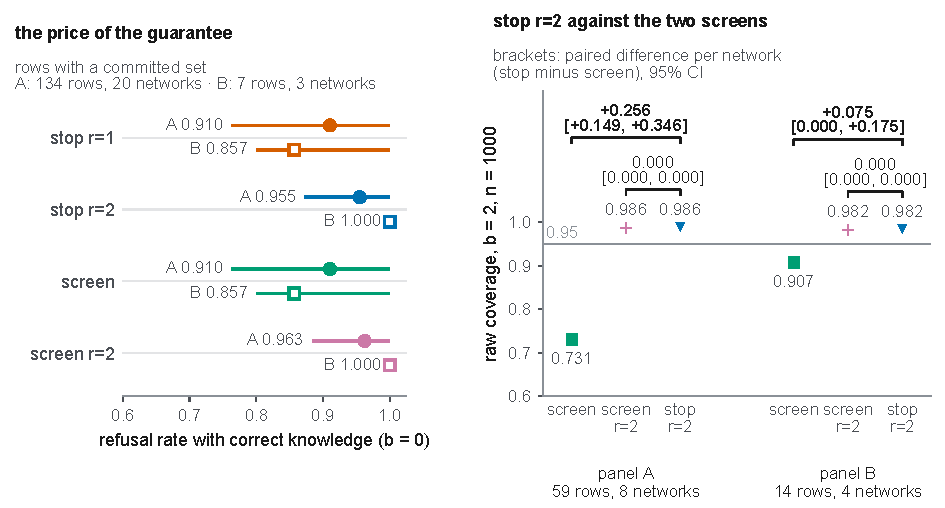
\includegraphics[width=\linewidth]{stop_refusal.pdf}
\caption{Left: with correct knowledge the stop rule and the one-claim screen refuse the same nine
analyses in ten; the 0.91 does not measure how demanding the rule is, it measures that the conclusion
rests on one claim. Right: at two wrong claims the two-claim rule covers more than the one-claim
screen and exactly as much as the pair screen.}
\label{fig:stop}
\end{figure}

The denominator must travel with the number: on committed queries outside the informative stratum
the rule refuses none (57 on Panel~A, 11 on Panel~B), and over all committed queries it refuses 0.639
(A) and 0.333 (B). \textbf{Q3 holds on the letter and is empty}: $\Lnf(\mathrm{STOP}_1)$ is below
$\Lnf(\Ir{1})$ in all four cells by 0.0003 to 0.0011, because read literally the rule widens on 97 to
99\,\% of informative queries. \textbf{Q5 holds}: at $b = 1$ it covers 0.979 and 0.979 on Panel~A
($n = 1000$, $20\,000$), 0.980 and 0.966 on Panel~B.

\prompt[conceito=regra-de-parada,dificuldade=0.7]{Give the three refusal rates of $\mathrm{STOP}_1$ at
$b = 0$ on Panel~A by denominator, and say which one Q4 was about.}{0.910 over the 134 informative
queries with a committed set (20 networks), the population of Q4, which predicted below 0.5; 0.639
over all committed queries; zero over the 57 committed queries outside the informative stratum, where
the class already identifies the effect.}

\begin{antes}
\antesq[screen-leave-k-out]{How much more does the two-claim rule cover than the one-claim screen at
$b = 2$, at which sample size, and on how many queries?}
\antesq[orcamento-retracao]{Where does a third of that difference come from?}
\antesq[screen-leave-k-out]{Against the pair screen, what is the difference?}
\end{antes}

\section{The starred comparison separates, then ties}

The comparison fixed on 7 September, $\mathrm{STOP}_2$ against SCREEN at $b = 2$ on Panel~A (59
committed informative queries, 8 networks), separates as Q2 predicted: $+0.256$ $[+0.149, +0.346]$ in
coverage at $n = 1000$ (0.986 against 0.731), $+0.269$ $[+0.163, +0.361]$ at $n = 20\,000$, and
$+0.305$ $[+0.182, +0.410]$ in the population (1.000 against 0.695). The interaction ceiling is 0.237
(A) and 0.286 (B). Q2 is supported as written, and two facts qualify it.

\begin{table}[!ht]
\centering\footnotesize
\caption{Where the $\mathrm{STOP}_2 - \mathrm{SCREEN}$ coverage gap comes from, Panel~A, $b = 2$,
$n = 1000$, committed informative queries. Source: \texttt{results/interval/TABLE1\_L95.md}, M1b
section.}
\label{tab:m1b-decomp}
\begin{tabular}{@{}lrrrr@{}}
\toprule
stratum & queries & share of replicates & gap inside & contribution \\
\midrule
interaction ($\rval = 2$, or a pair changes the result) & 14 & 0.24 & $+0.689$ & $+0.164$ \\
$\rval = 1$ (both policies refuse)                       & 34 & 0.58 & $+0.159$ & $+0.092$ \\
rest                                                     & 11 & 0.19 & $+0.005$ & $+0.001$ \\
\bottomrule
\end{tabular}
\end{table}

\textbf{About a third of the gap is the fallback, not the depth.} On the 34 queries with $\rval = 1$
both policies refuse, but the rule reports $\Ir{2}$ and the screen $\Ir{1}$, and with two wrong claims
$\Ir{2}$ covers more: $+0.092$ of the $+0.256$ (Table~\ref{tab:m1b-decomp}). Only the 14 interaction
queries measure depth. On Panel~B (14 queries, 4 networks) the gap is $+0.075$ $[+0.000, +0.175]$ at
$n = 1000$, all of it from 4 interaction queries, with an interval touching zero.

\textbf{A free screen at depth two ties exactly.} $\mathrm{STOP}_2$ against SCREEN2, both falling back
to $\Ir{2}$: coverage $+0.000$ $[+0.000, +0.000]$ at $n = 1000$, $-0.002$ $[-0.003, +0.000]$ at
$n = 20\,000$, zero on Panel~B. They decide differently on 5 of the 754 committed informative queries of
the five conditions ($141 + 162 + 73 + 161 + 217$), all of the example's class. The pre-fixed
comparison separated only because its free baseline stopped at depth one.

\textbf{Q1 failed by one query.} At $b = 1$, rule and screen differ on 2 of 162 committed queries
(1.23\,\%), both of the expected class: \texttt{Kampen\_2014}, ALN on PER, $Z = \{\mathrm{AFF},
\mathrm{SAN}\}$, $\rval = 3$; and \texttt{Schipf\_2010}, A on S, $Z$ empty, $\rval = 2$, where one
retraction makes the closed form return a non-empty optimal set for which the empty set is still valid.
Q2 and Q5 are supported, Q3 on the letter only, Q1 and Q4 falsified.

\prompt[conceito=orcamento-retracao,dificuldade=0.8]{Why does the $+0.256$ advantage of the two-claim
rule over the one-claim screen not measure only the value of certifying at depth two? Give the sample
size and the population line.}{Because the policies differ in two things: the depth of the certificate
and the budget of the fallback interval. On the 34 queries with $\rval = 1$ both refuse, but the rule
reports $\Ir{2}$ and the screen $\Ir{1}$; with two wrong claims $\Ir{2}$ covers more, and that stratum
contributes $+0.092$. Only the 14 interaction queries ($+0.164$) measure depth, and against a screen
that also tries pairs, with the same fallback, the difference is $+0.000$. The $+0.256$
$[+0.149, +0.346]$ is at $n = 1000$ on 59 queries and 8 networks; the population line of the same
contrast is $+0.305$ $[+0.182, +0.410]$.}

\begin{antes}
\antesq[frases-proibidas]{What does the pre-declared sentence turn the paper into?}
\antesq[regra-de-parada]{What survives M1b, measured?}
\antesq[screen-leave-k-out]{Which column is missing from the $\tau_b$ table of your draft?}
\end{antes}

\section{What survives, and the column your ranking table lacks}

Said without softening: \textbf{the sentence pre-declared on 7 September applies}. The starred
comparison separated against the one-claim screen and tied against the pair screen; at no depth we
measured does the stop rule compute something a leave-$k$-out screen does not. Nothing in the paper
may suggest that the radius, the certificate or the stop rule beats such a screen.

\begin{sonorio}[The tie, in the licensed form]
This is a measurement of when background-knowledge error is silent and what it costs. At every depth
we measured, the validity half of the sensitivity report matches a leave-$k$-out re-closure screen,
and the two differ only where a retraction changes the adjustment set while leaving it valid. We state
this as a property of the measure; what the report adds is the depth that was needed and the named
claims that witness it.
\end{sonorio}

What survives is measured, each number with its population. One wrong claim costs the committed
report 37 points of coverage (Panel~A, $n = 1000$: 0.967 to 0.597; 42 in the population), and the
knowledge interval restores coverage at 76 to 97\,\% of the class width ($\Lnf(\Ir{1})$ at $b = 1$,
0.758 to 0.974 over panels and sample sizes). Where an adjustment depends on knowledge, it almost
always rests on one claim (refusal 0.910; $\rnul$ at 1 or beyond 3 on 92.8\,\% of Panel~A's
established effects), so the report's most useful output is the \emph{name} of that claim; on the
ledger (a different harness: primary supplier, 157 exact rows, oracle CPDAG) the named claim was false on
58 of the 62 queries whose set was invalid at the truth (\texttt{results/ledger/CHECKS.md}, Table~8 in
Chapter~\ref{ch:frame}). The outline of 13 September
lists this framing as decision D9 and recommends accepting it rather than searching for a population
where conclusions rest on more claims, which would be selected for the answer. I recommend the same.

\textbf{The baseline your $\tau_b$ table is missing.} The ranking table of your draft
(\texttt{tab:tau} in \texttt{sections/06\_simulation.tex}) sets $\tau_b(\rval)$ against $\tau_b(\mathrm{SHD})$ and
$\tau_b(|\Kset|)$, two weak baselines. A reviewer who knows the area proposes the screen: the depth at
which leave-$k$-out re-closure first changes the set. By the argument above it never exceeds $\rval$
and equals it except where the set changes while staying valid (5 of 754 queries in M1b). The column
is unrun; your corruption states are stored, so it is cheap. I expect $\tau_b(\text{screen depth})$
close to $\tau_b(\rval)$; that is a prediction, not a measurement.

\begin{noprato}[Before the ranking table goes into the merged paper]
Add $\tau_b(\text{screen depth})$ on the same stored states and bootstrap. If it ties, state the
ranking as a property shared with the screen and say what the radius adds: the depth, the witness, the
certificate that no failure lies nearer.
\end{noprato}

\naopasse[orcamento-retracao]{Rebuild the decomposition of the starred comparison: queries, contribution
and mechanism per stratum. If you cannot say why the 34 queries with $\rval = 1$ contribute although both
policies refuse there, reread the paragraph on the fallback.}

\subsection*{Exercises}

\begin{exercicio}[metodo=estimation,conceito=regra-de-parada]
Before looking at the refusal table, you are given only the identity table for correct knowledge
($b = 0$), Panel~A, 134 informative committed queries: $\rval = 1$ on 0.910 of them and $\rval = 2$
on 0.045; no query differs between $\mathrm{STOP}_1$ and SCREEN. (a) Estimate the refusal rates of
$\mathrm{STOP}_1$, $\mathrm{STOP}_2$ and SCREEN. (b) Bound SCREEN2's from below, and say what the gap
between SCREEN2 and $\mathrm{STOP}_2$ can consist of. (c) Describe the population on which Q4
(refusal below 0.5) could have held.
\end{exercicio}
\begin{solucao}
(a) $\mathrm{STOP}_1$ refuses iff $\rval \le 1$: 0.910 (measured 0.910); $\mathrm{STOP}_2$ iff
$\rval \le 2$: $0.910 + 0.045 = 0.955$ (measured 0.955); SCREEN equals $\mathrm{STOP}_1$, no query
differing: 0.910. (b) Refusal implies trigger at the same depth, so SCREEN2 refuses at
least wherever $\mathrm{STOP}_2$ does: $\ge 0.955$. The excess can only be queries where a pair
retraction changes the set while $Z$ stays valid to depth two. Measured 0.963, so
$(0.963 - 0.955) \times 134 \approx 1$ query. (c) One where committed sets mostly survive every single
retraction, conclusions resting on two or more claims (larger chain components, denser knowledge near
the query). Here that is about one query in twenty; choosing such a population now would select for the
answer.
\end{solucao}

\begin{exercicio}[metodo=diagnosis,conceito=screen-leave-k-out]
A draft paragraph reads: \emph{``Our radius-based stop rule, which certifies the adjustment set up to
two retractions, improves coverage over leave-one-out screening by 25.6 points (0.986 vs.\ 0.731),
showing that the breakdown radius captures interactions between knowledge errors that a screen
misses.''} Diagnose every defect, with the number that exposes it, and say which sentence of
Chapter~\ref{ch:gamma} or this chapter should replace it.
\end{exercicio}
\begin{solucao}
(1) No population or sample size: $+0.256$ $[+0.149, +0.346]$ is Panel~A, $n = 1000$, 59 committed
informative queries on 8 networks; the population line is $+0.305$, and Panel~B's $+0.075$ touches zero.
(2) Depth is confounded with fallback: $+0.092$ comes from the 34 queries with $\rval = 1$ where both
policies refuse and differ only in widening to $\Ir{2}$ or $\Ir{1}$. (3) The conclusion is false at
matched depth: against the pair screen the difference is $+0.000$ $[+0.000, +0.000]$, with 5 of 754
queries decided differently, none unsafe. (4) ``Improves over'' is the forbidden claim that the radius
beats a leave-$k$-out screen. Replace the paragraph with this chapter's purple box, keeping the
one-claim contrast only with its sample size and decomposition.
\end{solucao}

\section*{Chapter map}
\begin{center}
\begin{tikzpicture}[node distance=0.6cm and 1.1cm]
\node[cmapc] (des) {7 Sep design:\\ policy rows};
\node[cmap, right=of des] (stop) {stop rule\\ $\mathrm{STOP}_r$};
\node[cmap, right=of stop] (scr) {leave-$k$-out screen\\ SCREEN, SCREEN2};
\node[cmapc, right=of scr] (frase) {pre-declared sentence\\ applies: a measurement};
\node[cmapr, below=of des] (ref) {refusal 0.910\\ with correct claims};
\node[cmapg, below=of stop] (sep) {separates: $+0.256$\\ ($n = 1000$) vs SCREEN};
\node[cmapr, below=of scr] (tie) {ties: $+0.000$\\ vs SCREEN2};
\node[cmap, below=of frase] (tau) {owed: screen-depth\\ column in $\tau_b$ table};
\draw[cedge] (des) -- node[above]{asks for} (stop);
\draw[cedge] (stop) -- node[above]{same at depth 1} (scr);
\draw[cedge] (scr) -- node[above]{tie triggers} (frase);
\draw[cedge] (des) -- node[left]{price cell} (ref);
\draw[cedge] (stop) -- node[left]{at $b = 2$} (sep);
\draw[cedge] (sep) -- node[above]{a third is fallback} (tie);
\draw[cedge] (frase) -- node[right]{implies} (tau);
\end{tikzpicture}
\end{center}

% =============================================================================
\chapter{16 September: what the cells mean, T3, and a bias in our own table}\label{ch:tables}

\begin{ideia}[The chapter in two sentences]
A cell of the price table answers one question: forced to cover honestly, how wide would this
procedure have to be, compared with discarding the knowledge? And the table of named reports, read
in full, shows that one retraction usually returns the analyst to the whole class, while the rule
that chose its rows biased the one column that looked most like Rosenbaum.
\end{ideia}

Two documents were written this morning, both in English and both on the branch:
\nolinkurl{rho_breakdown/table1_dossier_2026-09-16/}, a dossier of every Table~1 the results support,
and \nolinkurl{rho_breakdown/panelB_T3_2026-09-16/}, which opens one cell of the price table, prints the
named reports in full and audits how their rows were chosen.

\begin{armadilha}[Three numbering schemes]
The dossier's \textbf{T3} is M1's Table~2 (\texttt{results/interval/TABLE2\_REPORTS.md}), the paper's
future Table~2. The ``Panel~B'' of its recommended \textbf{T11} is the price table on M1's
\emph{Panel~A} (semi-synthetic), not M1's Panel~B. ``Table~3'' in the outline of 13 September is the
audit under wrong knowledge. Below, T-numbers are the dossier's and panels are M1's.
\end{armadilha}

\begin{antes}
\antesq[metrica-unica]{In the one-wrong-claim cell, what are $\lambda^{*}$ and the mean half-width of
the committed report, and how do they give 5.123?}
\antesq[metrica-unica]{How does a procedure earn an $\Lnf$ above 1?}
\end{antes}

\section{Opening one cell}

Take the one-wrong-claim cell of Panel~A at $n = 1000$: 359 queries, twenty seeds each, 7,180
replicates. For each replicate $i$ a procedure reports an interval with midpoint $m_i$ and half-width
$h_i$, and $\lambda_i = |\tau - m_i| / h_i$ is the factor by which that interval must be stretched about
its own midpoint to reach the true effect. Below 1, it already covers. Take $\lambda^{*}$, the 95th
percentile of the $\lambda_i$ over the cell: stretching every interval by $\lambda^{*}$ makes 95\,\% of
them cover. Average the stretched widths $2\lambda^{*}h_i$ and divide by the same quantity for the
whole class.

\begin{medido}[The cell, recomputed from replicates by \texttt{make\_figs.py}]
Script \nolinkurl{rho_breakdown/panelB_T3_2026-09-16/make_figs.py}, reading
\texttt{results/interval/replicates.csv.gz}. Panel~A, $b = 1$, $n = 1000$, 7,180 replicates.

\medskip
\begin{tabular}{@{}lrrrr@{}}
procedure & $\lambda^{*}$ & mean half-width & calibrated width & $\Lnf$ \\
\midrule
PLAIN, the committed report & 20.416 & 0.3855 & 15.7397 & \textbf{5.123} \\
$\Ir{1}$, one revision       & 1.000  & 1.3064 & 2.6129  & \textbf{0.851} \\
BLANKET, the whole class     & 1.000  & 1.5361 & 3.0721  & 1.000 \\
\end{tabular}

\medskip
$15.7397 / 3.0721 = 5.123$ and $2.6129 / 3.0721 = 0.851$. At $n = 20\,000$ the same two cells read
14.368 and 0.758: more data narrows a wrongly centred interval without moving it.
\end{medido}

The committed report is the narrowest interval in the cell (mean half-width 0.39 against 1.54 for the
class) and the most expensive once it is required to be right. \figref{fig:t3-why} shows why: the
stretch is about the interval's own midpoint, so a narrow interval centred on the effect the wrong
graph implies has to be compensated on both sides.

\begin{figure}[!ht]
\centering
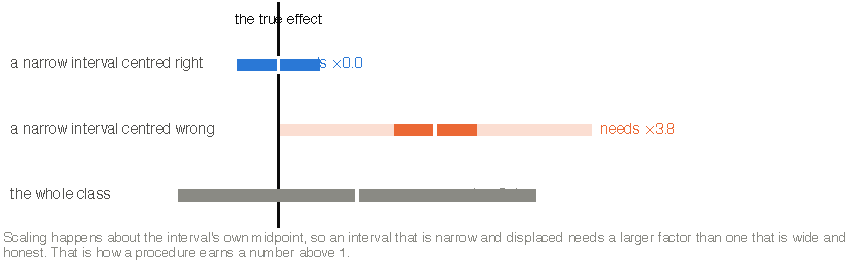
\includegraphics[width=0.74\linewidth]{t3_f5_why_above_one.pdf}
\caption{Schematic. A narrow interval centred away from the truth needs a larger factor than a wide
honest one; that is the only way a procedure lands above 1, wider than discarding the knowledge.}
\label{fig:t3-why}
\end{figure}

\textbf{The reproduction.} The script reimplements the $\Lnf$ pipeline from \texttt{replicates.csv.gz}
and \texttt{rows.csv} and asserts that all 27 Panel~A cells of \texttt{TABLE1\_L95.md} at $n = 1000$
(nine procedures, three columns) come out to three decimals; I reran it today and it passes. The filter
that makes it reproduce: a query enters a column iff it is informative \emph{and} its realised $b$ is
non-empty (391, 359, 131 queries).

\begin{armadilha}[\texttt{profiles.jsonl} is the wrong join key for cells]
My first attempt joined the replicates on \texttt{results/interval/profiles.jsonl} and got 0.180 for
PLAIN at $b = 0$ instead of 0.464. That file holds 934 profiles, only for queries whose analyst graph
commits to a set, so the join silently rebuilt the committed-set secondary table, whose cell really is
0.180 on 134 queries. A correct number for the wrong population; the comparison with the published
cell is what caught it.
\end{armadilha}

\prompt[conceito=metrica-unica,dificuldade=0.7]{In the Panel~A, $b = 1$, $n = 1000$ cell, give
$\lambda^{*}$ and the mean half-width of the committed report and of the class, and compute $\Lnf$ of
the committed report.}{Committed report: $\lambda^{*} = 20.416$, mean half-width 0.3855, calibrated
width $2 \times 20.416 \times 0.3855 = 15.74$. Class: $\lambda^{*} = 1.000$, mean half-width 1.5361,
calibrated width 3.072. $\Lnf = 15.74 / 3.072 = 5.123$, over 7,180 replicates of 359 queries.}

\begin{antes}
\antesq[testemunha]{Of the nine certifiable declared queries, how many break under some retraction
of up to three claims, and how many of the seventeen fitted-coefficient queries break at the first?}
\antesq[r0-binario]{Why did the pre-registered Figure~1 rule return no candidate?}
\antesq[nulidade]{Can a query have $\rval = 1$ and $\rnul$ ``never''?}
\end{antes}

\section{T3 in full: a cliff, not a curve}

T3 has 26 rows under the recovering set, estimates at $n = 20\,000$ and seed 0: the nine declared
queries with a valid status and 17 frame queries on the four fitted-coefficient networks. Three declared
queries are excluded with their reasons (\texttt{M-bias}: the published diagram is not a DAG;
\texttt{Schipf\_2010}, TT on T2DM: the outcome is not a possible descendant; \texttt{confounding}: the
treatment has no undirected edge). Read twice, the table says four things.

\textbf{The published analyses are robust and the sampled ones are not.} Eight of the nine declared
queries are unbroken by any retraction to depth three; the exception is \texttt{mediator}, a four-node
textbook diagram. On the fitted networks, 16 of 17 queries have $\rval = 1$. The mechanism is the frame:
a pair is admitted beside an undirected edge, where knowledge can matter, so the measured population
is close to the complement of the queries the source papers were written to answer. That is an
applicability statement for the paper's evaluation section, not a result.

\textbf{The sensitivity curve is a single step.} On 16 of T3's 17 informative rows (the 16 informative
fitted queries and \texttt{mediator}) the interval after one retraction equals the whole-class interval
to four decimals. The exception is again
\texttt{mediator}, whose first retraction covers 57\,\% of the class and whose second saturates it. All
the identifying power the knowledge supplies sits in one claim, and withdrawing it returns the analyst
to where they would be with no knowledge. This is why the pre-registered Figure~1 rule (both radii in
$\{2, 3\}$ and a plateau before the break) found nothing on real coefficients: the shape it looked for
is not in the data, and the declared and applied rows that did have radii 2 or 3 widened 27 to 34 times
before breaking. The companion's recommended figure (its candidate F-A) draws this cliff; the
version on the full eligible pool is in the next section.

\textbf{The null radius and the validity radius are different numbers.} On \texttt{mediator} the set
fails after one retraction and the interval reaches zero after two. On \texttt{ecoli70} eutG $\to$
lacY and both \texttt{magic-niab} G1217 queries, $\rval = 1$ and $\rnul$ is ``never'': the set breaks,
the sign does not. On several fitted rows the band at seed 0 contains zero at budget zero (0 from the
band, 1 from the population): no conclusion to break at that sample size. A sentence about $\rnul$
must name its reading (population, one seed, range over twenty), and a figure's axis label must say
whether it shows conclusions or validity.

\textbf{Why the one- and two-revision columns look identical.} $\Ir{r}$ grows with $r$ and is capped by
the class interval. Of the 303 committed queries under the recovering set, 281 (92.7\,\%) print the
same interval at both budgets: on 76 the class interval is a point, on 205 the first revision already
returns the class. The second column carries information on 20 queries, on \texttt{insurance},
\texttt{Polzer\_2012}, \texttt{Kampen\_2014}, \texttt{sachs}, \texttt{Schipf\_2010} and
\texttt{mediator}, all but the last excluded from T3 by its real-coefficient rule. Replace the
two-revision column with the class interval, and the identity becomes visible as the finding.

\prompt[conceito=r0-binario,dificuldade=0.75]{State the one-claim cliff as measured on T3, name the
exception, and say what it did to the pre-registered Figure~1 rule.}{On 16 of the 17 informative T3
rows the interval after one retraction equals the whole-class interval to four decimals; the exception
is \texttt{mediator}, where one retraction covers 57\,\% of the class and two saturate it. The
pre-registered rule wanted both radii in $\{2, 3\}$ and a plateau before the break on a real-coefficient
network under truthful knowledge; the curve is a single step, so no row qualified, and the rows with
radii 2 or 3 widened 27 to 34 times before breaking.}

\begin{antes}
\antesq[pre-registro]{T3 prints 17 of the 294 eligible sampled queries. By which two rules, and which
one is indefensible?}
\antesq[pre-registro]{What share of printed, dropped and eligible queries has a finite null radius?}
\antesq[testemunha]{Which claim of T3 survives the selection audit?}
\end{antes}

\section{A selection bias in our own table}

T3 is a selection made by two rules. The funnel is the whole path under the recovering set; the
counts are in \texttt{results/ledger/TABLE0\_FUNNEL.md} or were recounted from
\texttt{results/interval/rows.csv} and \texttt{profiles.jsonl} by
\nolinkurl{rho_breakdown/panelB_T3_2026-09-16/make_exhaustive.py}, which first checks the 26 printed
rows cell by cell against \texttt{table2.json}.

\begin{center}\footnotesize
\begin{tabular}{@{}rp{6.2cm}p{6.6cm}@{}}
\toprule
count & stage & what leaves, and why \\
\midrule
39 / 33 / 27 & networks parsed / with a frame / swept & over 500 nodes, or every component over the questionnaire cap \\
80{,}132 & candidate pairs, from observables only & \\
648 & pairs sampled (at most 20 per network) & \\
537 & rows: 528 frame rows in the swept networks + 9 declared & \\
303 & commit to an adjustment set (9 declared, 294 sampled) & 234: on the analyst's graph the outcome cannot descend from the treatment \\
37 & \textbf{rule 1}: fitted coefficients only & 257 on the 23 semi-synthetic networks; \textcolor{verdesc}{defensible}, not in the caption \\
17 & \textbf{rule 2}: finite $\rnul$ first, then frame order, five per network & 20; sorts on the outcome it illustrates: \textcolor{vermesc}{indefensible} \\
\midrule
26 & T3 = 9 declared + 17 sampled & \\
\bottomrule
\end{tabular}
\end{center}

\textbf{Rule 1 is defensible}: on the 23 semi-synthetic networks the effect size is one we drew, and a
named report would present it as a real analysis. It belongs in the caption.

\textbf{Rule 2 is not.} The Table~2 block of \texttt{experiments/interval\_tables.py} (line 1136) sorts the
eligible queries of each network by \texttt{(r0\_pop == CENSORED, frame\_index)} and keeps the first five.
A finite null radius is exactly what the table exists to illustrate.

\begin{medido}[The bias, \texttt{rho\_breakdown/panelB\_T3\_2026-09-16/make\_figs.py} (rerun 16 September)]
Queries on the four fitted networks with a committed set: 37 eligible, 17 printed, 20 dropped (9 on
\texttt{magic-niab}, 8 on \texttt{magic-irri}, 3 on \texttt{ecoli70}). Finite population null radius:
13 of 17 printed (76\,\%), 3 of 20 dropped (15\,\%), 16 of 37 eligible (43\,\%).
\end{medido}

I have to be exact about whose defect this is. The ordering was not chosen after seeing the answer: it
is written in \S6 of \texttt{results/interval/PREREGISTRATION.md} (``finite r0 first, then frame
order''), before any row existed, and the header of \texttt{TABLE2\_REPORTS.md} states it. It was still
the wrong rule, because it sorts on the outcome, and nobody measured its effect until this morning. The
$\rnul$ column of T3 is not representative of the population it was drawn from.

\begin{noprato}[The fix, one line]
In \texttt{experiments/interval\_tables.py}, sort the candidates by \texttt{frame\_index} alone (drop
the \texttt{r0\_pop == CENSORED} term), or better, print all 37 eligible queries so the inclusion rule
has nothing in it a reader must trust. Put rule 1 and the eligible count in the caption. Draw the
figure on the 37, not on the 17.
\end{noprato}

\textbf{What the selection did not bias.} The cliff survives. On all 26 informative queries of the 37
eligible, one retraction returns the whole-class interval (16 of 16 printed, 10 of 10 dropped). Over
all 294 committed sampled queries on 27 networks, 226 are informative; on 205 the one-retraction
interval equals the class interval to four decimals, and on 211 (93\,\%) it covers more than 90\,\% of
the class width. \figref{fig:t3-pool} draws F-A on the 37 eligible queries, printed ones marked,
including the 11 rows where nothing moves, which T3 hides.

\begin{figure}[!ht]
\centering
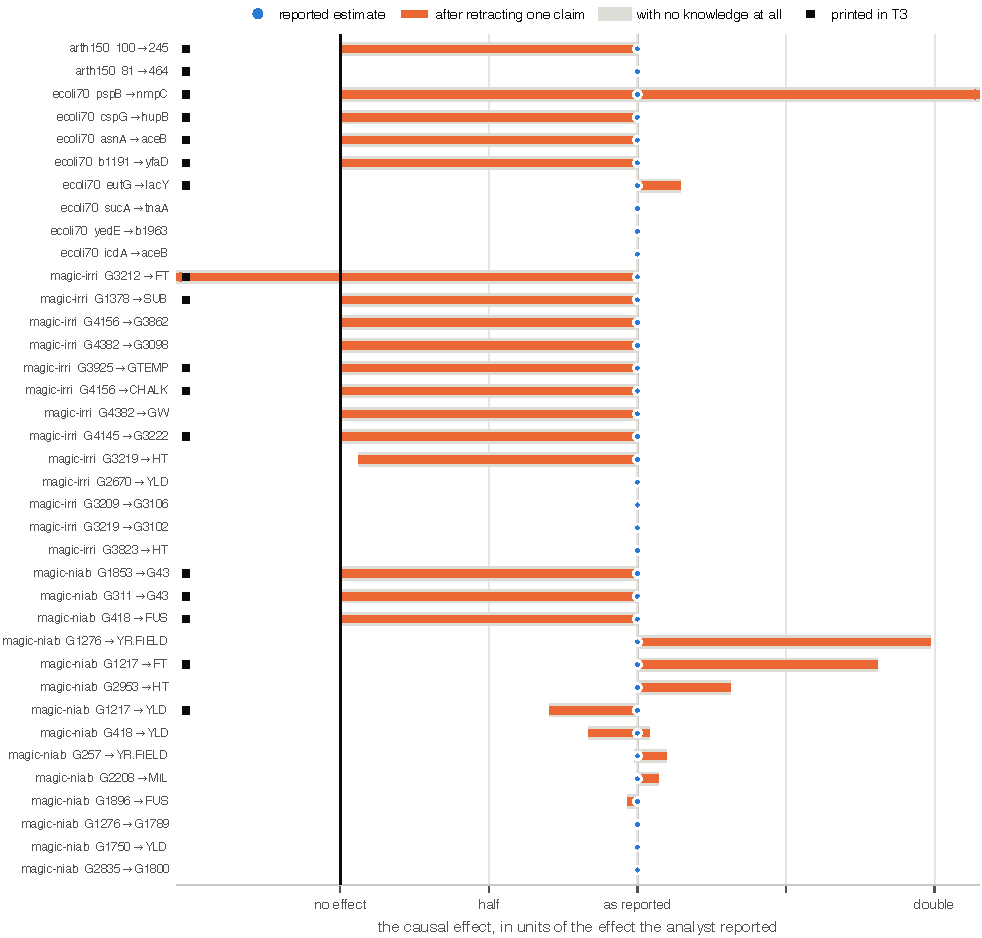
\includegraphics[width=0.60\linewidth]{t3_f11_pool_dumbbell.pdf}
\caption{All 37 eligible fitted-coefficient queries, printed ones marked with a square: the cliff holds
on the dropped queries too, and the rows with no bar (the class already pins the effect) are the honest
counterweight the printed table leaves out.}
\label{fig:t3-pool}
\end{figure}

\prompt[conceito=pre-registro,dificuldade=0.75]{Give the three finite-null-radius shares of the T3
audit with their denominators, the line that produced the bias, and the fix.}{Finite population
$\rnul$ on 13 of 17 printed queries (76\,\%), 3 of 20 dropped (15\,\%), 16 of 37 eligible (43\,\%). The
sort key \texttt{(r0\_pop == CENSORED, frame\_index)} in \nolinkurl{experiments/interval_tables.py} puts
finite null radii first before taking five per network; the rule is in \S6 of the pre-registration.
Fix: sort by \texttt{frame\_index} alone, or print all 37, and state the real-coefficient rule and the
eligible count in the caption.}

\begin{antes}
\antesq[dois-paineis]{Which candidate does the dossier recommend as Table~1, and what are its two
panels?}
\antesq[decisoes-abertas]{What blocks the abstract of 18 September, according to the dossier?}
\end{antes}

\section{The Table 1 dossier}

The dossier states eleven live claims before any table, each with evidence, significance, nearest
prior art and falsifier (\nolinkurl{rho_breakdown/table1_dossier_2026-09-16/sections/02_claims.tex}).

\begin{center}\footnotesize
\begin{tabular}{@{}lll@{}}
\toprule
& claim & what carries it \\
\midrule
C1 & nobody prices a structural assumption & framing; \textbf{novelty search never run in this wording} \\
C2 & computable from the analyst's inputs & monotonicity audit: 5,000 pairs, 0 violations (bound 0.06\,\%) \\
C3 & claims are the safe unit, hops are not & 3,014 certifiable rows: 0 over-certifications against 39 \\
C4 & the price of a wrong claim & $\Ir{1}$ at 0.851 of the class, premium at zero (Ch.~\ref{ch:gamma}) \\
C5 & the tie with the free screen & $+0.000$ at matched depth (Ch.~\ref{ch:m1b}) \\
C6 & refusal where knowledge matters & 0.910 of 134 committed informative queries \\
C7 & locality in claims, not hops & primary supplier: hop reading above claim depth on 21 of 157 \\
C8 & applicability, as a limit & 8 of 9 declared queries unbroken to depth 3 \\
C9 & the class must be correct & estimated CPDAG: over-certification on 14 of 38 (Ch.~\ref{ch:pest}) \\
C10 & suppliers are an error process & invalid set 0.298 at 72B, 0.288 at 7B \\
C11 & ranking by survival & your $\tau_b$ table; screen column owed \\
\bottomrule
\end{tabular}
\end{center}

\textbf{Thirteen candidates} (T1 to T13, with a variant T1b) are typeset with the numbers that exist and
scored against three requirements (readable after the abstract; verifies the claims we make; compares
with the literature inside the float) and six constraints each earlier design paid
for: one calibrated metric, one population per panel, a row that loses where it must, no discrimination
column, no model family as subject, nothing internal in the float. \textbf{The recommendation is T11},
one float with two panels on two named populations. Its first panel is the certificate ladder over the
3,014 certifiable rows of eleven knowledge conditions on 27 networks (902 committed sets invalid at the
truth): counting claims asserted over-certifies on 729, the separation rule on 15, the hop radius on 39,
the claim radius on 0. Its second panel is the price table at $n = 1000$ with the leave-one-out screen as
a row, and the refusal rate (0.910 of 134) under the float with its own denominator. T3 becomes Table~2,
the policy table T8 becomes Table~3 or prose, your ranking table T4 stays in its section with the screen
column added, and the decision table T5 is the best candidate for the first figure.

Two defects were found and fixed while the dossier was written, each the kind it warns against. The
first draft of T8 and of T11's second panel filled the two-wrong-claim cells of the screen and
stop-rule rows from M1b's 59 committed queries beside cells from the price table's 131: two populations
in one row. And the ladder's 15 over-certifications had been attributed to the leave-one-out screen;
they belong to the separation rule (the screen never over-certifies relative to the stop rule, 0
exceptions in 2,212 rows). A reconciliation, not a defect: my review notes quoted the depth-one screen
gap as $+0.305$, the dossier as $+0.256$; both are in \texttt{TABLE1\_L95.md}, the population line and
the $n = 1000$ line, and every quotation now carries its sample size.

\begin{noprato}[Blocking before the abstract on 18 September]
\textbf{C1's novelty search has never been run in the wording the claim uses.} The searches on record
were pointed at latent-causal representation learning and at Taeb, Guo and Henckel, not at the
sensitivity-analysis lineage C1 says does not already price this, and the statement that Guo and Perkovi\'c never
perturb the knowledge rests on a paper I have not read in full. Either the search runs before the
abstract, or C1 is narrowed to what was searched and the abstract says the narrower thing.
\textbf{The author list must be settled by 18 September}; Chapter~\ref{ch:merge} quotes the rule.
\end{noprato}

\prompt[conceito=dois-paineis,dificuldade=0.7]{Which Table~1 does the dossier recommend, what are its
two panels with their populations, and what blocks the abstract of 18 September?}{T11. Panel one is the
certificate ladder over 3,014 certifiable rows (eleven knowledge conditions, 27 networks, 902 sets invalid
at the truth): the claim count over-certifies on 729, the separation rule on 15, the hop radius on 39,
the claim radius on 0. Panel two is the price table on M1's Panel~A at $n = 1000$ (391, 359, 131
informative queries) with the leave-one-out screen as a row, and the refusal rate 0.910 of 134 printed
under the float with its own denominator. Blocking: the novelty search for C1 has never been run in the
wording of the claim, and the author list must be settled by 18 September.}

\naopasse[pre-registro]{Name the sort key that biased T3, say what it sorts on, and explain in one
sentence why it biases the $\rnul$ column but not the claim that one retraction returns the class
interval. If you cannot, reread the paragraph ``What the selection did not bias''.}

\subsection*{Exercises}

\begin{exercicio}[metodo=table-reading,conceito=nulidade]
Five rows of T3 (recovering set; bands at $n = 20\,000$, seed 0; class interval from the population;
$\rnul$ as population / band at seed 0 / range over 20 seeds).

\smallskip
{\footnotesize\setlength{\tabcolsep}{3pt}
\begin{tabular}{@{}lrllllc@{}}
\toprule
query & true & one revision & two revisions & class & $\rnul$ & $\rval$ \\
\midrule
mediator, X $\to$ Y & $-2.603$ & $[-2.623, -1.109]$ & $[-2.623, 0.000]$ & $[-2.603, 0.000]$ & 2 / 2 / 2 & 1 \\
ecoli70, eutG $\to$ lacY & $0.309$ & $[0.277, 0.377]$ & $[0.277, 0.377]$ & $[0.309, 0.354]$ & never / $>$3 / $>$3 & 1 \\
magic-niab, G418 $\to$ FUS & $0.003$ & $[-0.022, 0.011]$ & $[-0.022, 0.011]$ & $[0.000, 0.003]$ & 1 / 0 / 0..1 & 1 \\
ecoli70, pspB $\to$ nmpC & $-0.108$ & $[-0.531, 0.026]$ & $[-0.531, 0.026]$ & $[-0.525, 0.000]$ & 1 / 1 / 1..3 & 1 \\
arth150, 81 $\to$ 464 & $0.256$ & $[0.097, 0.265]$ & $[0.097, 0.265]$ & $[0.256, 0.256]$ & $>$3 / $>$3 / $>$3 & $\ge 2$ \\
\bottomrule
\end{tabular}}

\smallskip
(a) On which row do the two revision columns differ, and what does that say about the cliff? (b) Which
row has $\rval = 1$ and $\rnul$ ``never'', and why is that not a contradiction? (c) On which row does the
null radius depend on the reading, and how should a sentence quote it? (d) Which row must be left out of
``one retraction returns the class interval'', and why?
\end{exercicio}
\begin{solucao}
(a) \texttt{mediator}: one revision reaches $-1.109$, two reach zero, the class. It is the only row
where the first retraction stops short of the class (57\,\%), so the only one with a second step. (b)
eutG $\to$ lacY. $\rval$ is about the set (one retraction makes $Z$ invalid); $\rnul$ is about the sign
(every graph of the class gives an effect in $[0.309, 0.354]$). Validity breaks, the conclusion does
not. (c) G418 $\to$ FUS: population 1, seed 0 gives 0, range 0 to 1. The true effect is 0.003, so at
$n = 20\,000$ the band usually contains zero before any retraction; quote ``population null radius 1''
or the range, never a bare ``1''. pspB $\to$ nmpC (1 to 3 over seeds) needs the same care. (d) arth150,
81 $\to$ 464: the class interval is a point, so the query is not informative; its band is wide from
sampling alone.
\end{solucao}

\begin{exercicio}[metodo=rewriting,conceito=pre-registro]
T3's current caption reads, in part: \emph{``Sensitivity reports on twenty-six named analyses. \dots
$r_0$ is the null radius, the number of revisions after which the interval contains zero \dots
$r_{\mathrm{val}}$ is the breakdown radius \dots Knowledge: the recovering set; estimates at
$n = 20\,000$, first seed.''} Rewrite it as it should be printed once the fix is applied (all 37
eligible sampled queries shown), so that a reviewer can check the inclusion rule, the counts and the
two radii without opening any file. No internal vocabulary.
\end{exercicio}
\begin{solucao}
\emph{``Sensitivity reports on named analyses. Above the line, the nine published analyses whose
authors declared a treatment and an outcome (three more are excluded: one diagram is not acyclic, in one
the outcome cannot descend from the treatment, in one no claim bears on the treatment); structure as
published, parameters drawn. Below, all 37 sampled queries on the four networks with coefficients fitted
to real data whose analyst graph commits to an adjustment set; networks with drawn parameters are not
shown, since their effect sizes would be ours. Intervals: every effect identified after retracting at
most one claim, and over the whole equivalence class. Null radius: retracted claims until the 95\,\%
band contains zero (population, and range over twenty samples). Validity radius: retracted claims until
the adjustment set is no longer valid. Estimates at $n = 20\,000$.''} What changed: both inclusion rules
and the eligible count are stated, nothing is selected on the outcome, the class interval replaces the
two-revision column, the null radius carries its reading, and ``breakdown radius'' is renamed so it
cannot be confused with the null radius.
\end{solucao}

\section*{Chapter map}
\begin{center}
\begin{tikzpicture}[node distance=0.6cm and 1.1cm]
\node[cmapc] (cell) {a cell: $\lambda^{*}$, calibrated\\ width, ratio to class};
\node[cmap, right=of cell] (t3) {T3: 26 named\\ reports};
\node[cmapg, right=of t3] (cliff) {cliff: one retraction\\ returns the class};
\node[cmapr, below=of t3] (bias) {rule 2 sorts on $\rnul$:\\ 76\,\% vs 43\,\% vs 15\,\%};
\node[cmapg, below=of cliff] (pool) {not biased: 26/26,\\ 211 of 226};
\node[cmap, below=of cell] (fix) {fix: frame order\\ or all 37};
\node[cmapc, right=of pool] (t11) {dossier: T11;\\ C1 search blocks};
\draw[cedge] (cell) -- node[above]{prices} (t3);
\draw[cedge] (t3) -- node[above]{shows} (cliff);
\draw[cedge] (t3) -- node[left]{selected by} (bias);
\draw[cedge] (bias) -- node[above]{repaired by} (fix);
\draw[cedge] (cliff) -- node[right]{audited on} (pool);
\draw[cedge] (pool) -- node[above]{feeds} (t11);
\end{tikzpicture}
\end{center}


\part{Your draft and ours}
% =============================================================================
\chapter[Your draft, read against the measurements]{Your draft, read against\\ the measurements}
\label{ch:review}

I read your draft of 16 September as a referee would and against everything in the previous chapters, and
its theory was re-implemented from the definitions and searched for counterexamples. None was found: the
mathematics looks right, and every finding below is about what the text says. The numbers printed in your
draft were not audited in that pass. Each item gives where it sits, why it matters, and the fix.

\begin{ideia}[The review in two sentences]
Keep the object, the fixpoint definition and the reporting discipline as they are. Fix the positioning
against the paper you build on, the conditions the text drops, and prose that claims more than its table.
\end{ideia}

\begin{antes}
\antesq[espaco]{Which of your structural results does the foundation paper state to be false for
MPDAGs in general?}
\antesq[distancia-em-saltos]{Is there a formula for $d(G, H)$ on your space that needs no search?}
\end{antes}

\section{What the draft gets right}

\textbf{The object, in the right geometry.} Definition~1 by the fixpoint test is a real contribution:
Appendix~A.1 shows with minimal witnesses (the collider on a three-node chain, $K_4$ minus an edge with
one claim) why the two obvious filters are unsound, and covers are computed from model inclusion rather
than from a conjectured characterisation.

\textbf{The clinician sentence} in \S4.4 is the best-written sentence of the draft, and it makes the
object contestable by a domain expert. It belongs on page one.

\textbf{The reporting discipline} of \S5.4 is already the one our protocol uses: statuses on a frozen
instance list rather than filters, censoring rather than dropping, no numeric radius for an unreachable
failure, the two corruption arms never merged. \S6 states the observables-only invariant of
Chapter~\ref{ch:vocabulary} in one sentence. And Appendix~B's E3 is designed to refute rather than to
confirm («agreement proves nothing; only disagreement would be a theorem»), which is the right
epistemics for a verified-not-proved property.

\begin{medido}[Your theory, re-implemented from Definitions 1 to 3]
The space, the order, the covering relation and $d$ were rebuilt using only \texttt{MPDAG},
\texttt{apply\_orientations} and \texttt{enumerate\_dag\_extensions} from \texttt{src/\allowbreak bkrobust/\allowbreak demo/\allowbreak },
never the search or SAT code. Scale: 1,375 spaces, about 61,000 knowledge states, 9,648,249 ordered
pairs, 46,698 covering pairs, 188,116 anti-exchange triples (39,402 of them on states whose undirected
component is not chordal). Retraction-only radius equal to the brute-force radius on 8,161 of 8,161
instances; 599 of 599 nearest failing states reachable by retractions; the SAT clause set has 1,858
models for 1,858 space elements. \textbf{No counterexample to any checkable statement.} The check shares
your Meek and extension primitives, so a bug there would be invisible to it. From my review notes of 16
September; not in the branch.
\end{medido}

% -----------------------------------------------------------------------------
\begin{antes}
\antesq[espaco]{Where in the draft is the anti-exchange property stated?}
\antesq[gac-backdoor]{Which paragraph of the draft computes radii for sets other than the optimal one?}
\end{antes}

\section{The theory: what the text says}

\figref{fig:review-chain} is the dependency chain as the appendix proves it. Three results are
unconditional; four inherit the open case of the anti-exchange property; and the property itself is
the one statement the reader is never shown.

\begin{figure}[htbp]
\centering
\begin{tikzpicture}[font=\scriptsize\sffamily]
\node[cmapr] (ae) at (4.4,0) {anti-exchange:\\ stated nowhere, 4 × ??};
\node[cmap] (l2) at (4.4,-1.0) {Lemma 2: a cover\\ adds one orientation};
\node[cmap] (ps) at (4.4,-2.0) {Property 1: upper\\ semimodularity};
\node[cmap] (l3) at (4.4,-3.0) {Lemma 3: the join\\ is no farther};
\node[cmap] (p1) at (4.4,-4.0) {Prop.~1: monotone\\ reachability};
\node[cmapg] (l1) at (0,-1.0) {Lemma 1: order\\ identification};
\node[cmapg] (t2) at (0,-2.0) {Theorem 2:\\ join-semilattice};
\node[cmapg] (t1) at (0,-4.0) {Theorem 1: failure\\ upward-closed};
\node[cmapw] (tgh) at (9.0,0) {Taeb--Guo--Henckel, Prop.~9:\\ all MPDAGs on $V$, not graded};
\node[cmap] (gr) at (9.0,-1.0) {graded, rank $|\Kset_G|$};
\node[cmap] (cf) at (9.0,-2.0) {closed form\\ $d = |\Kset_G \triangle \Kset_H|$};
\node[cmap] (se) at (9.0,-4.0) {retraction-only search;\\ E1 counts equal hops};
\node[cmapc] (drop) at (9.0,-3.0) {condition dropped in abstract,\\ contributions, conclusion, \S5.3};
\draw[cedge] (ae) -- node[right]{via Edelman--Jamison} (l2);
\draw[cedge, densely dashed] (l1) -- node[above]{not cited there} (l2);
\draw[cedge] (l2) -- (ps);
\draw[cedge] (t2) -- (ps);
\draw[cedge] (ps) -- (l3);
\draw[cedge] (l3) -- (p1);
\draw[cedge] (t1) -- (p1);
\draw[cedge] (l2) -- (gr);
\draw[cedge] (l2) -- (cf);
\draw[cedge] (p1) -- (se);
\draw[cedge] (se) -- node[right]{stated as unconditional} (drop);
\draw[cedge, densely dashed, vermesc] (tgh) -- node[right]{skeleton varies there} (gr);
\end{tikzpicture}
\caption{Green results hold unconditionally; every white box inherits the anti-exchange property,
which the draft never states. The foundation paper's non-gradedness is about a larger poset, and the
draft does not yet say so.}
\label{fig:review-chain}
\end{figure}

\subsection*{1. The foundation paper states non-gradedness for a larger poset}

\emph{Where.} Appendix~A calls $\rho(G) = |\mathrm{dir}(G)| - |\mathrm{dir}(\Chat)|$ a rank function «so
the order is graded», Property~1 is upper semimodularity, and Theorem~2 makes the space a
join-semilattice. \emph{Why.} Proposition~9 of Taeb, Guo and Henckel states that the model-oriented poset
of MPDAGs on $|V| \ge 4$ vertices is not graded, and the paragraph after it says the poset is neither upper
nor lower semimodular, has no semilattice structure, and has no explicit graphical characterisation of
its covering relation; a referee who knows that paper reads Appendix~A as a contradiction. \emph{Fix.}
Say why both hold, in one paragraph of \S5.1 and one sentence of Appendix~A.

\begin{fonte}[Taeb, Guo and Henckel, arXiv:2511.10625v3, \S4.5 and Appendix D.3]
Their poset contains every MPDAG on $V$, from the empty graph to the complete undirected one, and covers
can change adjacencies: in their Example~2 two neighbours of the same graph differ from it by one edge
and by $n-1$ edges, and the proof of Proposition~9 compares two maximal chains of lengths 3 and 5 in
which a covering step removes an edge. On a common skeleton their Proposition~8 reduces the order to $[G] \subseteq [H]$,
which is yours, and their pseudo-rank (Definition~7, directed edges plus twice the undirected ones) equals
$2m - |\mathrm{dir}(G)|$ on a skeleton with $m$ edges: your rank, negated and shifted.
\end{fonte}

The paragraph needs five sentences, and it turns the largest liability of the draft into its clearest
positioning statement.

\begin{sonorio}[A paragraph for \S5.1]
These results do not contradict Proposition 9 of Taeb, Guo and Henckel (2025), which shows that the
model-oriented poset of all MPDAGs on four or more vertices is not graded, is not a semilattice and is
not semimodular. Their poset lets a covering step change the skeleton. The space studied here fixes the
skeleton and the v-structures of $\widehat{C}$, so only orientations vary. On it the join exists
unconditionally (Theorem 2), and gradedness and upper semimodularity hold under Conjecture 1, with their
pseudo-rank reducing to $2m - |\mathrm{dir}(G)|$.
\end{sonorio}

\subsection*{2. The anti-exchange property is never stated}

\emph{Where.} Four \verb|\Cref{prop:antiexchange}| calls (\S7, the proof of Lemma~2, the heading of
Appendix~A.3, the E3 paragraph of Appendix~B) point at a label that exists nowhere, so the compiled PDF
prints «??» four times, including the heading «A.3 Status of ??». \emph{Why.} The reproducibility
statement promises that the single unproved property is isolated in A.3, and the reader finds a section
about a statement they have never seen. \emph{Fix.} One environment, which also repairs the four
references.

\begin{noprato}[The statement, as \texttt{THEOREMS.md} §4c gives it]
Add to Appendix~A a \texttt{conjecture} environment (your macros define it) carrying
\texttt{\textbackslash label\{prop:antiexchange\}}: \emph{for a closed set $S$ of orientations and
distinct orientations $x, y \notin S$, if $y \in \mathrm{cl}(S \cup \{x\})$ then $x \notin \mathrm{cl}(S
\cup \{y\})$}. Its reading in words: no two distinct orientations are perfectly correlated across the
represented DAGs. Calling it a conjecture matches A.3, where Case~B is open.
\end{noprato}

\subsection*{3. Your theorems make the distance a closed form}

\emph{Where.} Definition~2 defines $d$ as a shortest path, and Appendix~C's «Against a naive count»
argues that counting the assertions that differ understates $d$. \emph{Why.} Lemma~2 and Theorem~2 give
$d(G, H) = |\Kset_G \triangle \Kset_H|$: each covering step changes $\Kset$ by exactly one orientation,
so $d \ge |\Kset_G \triangle \Kset_H|$; and $J = G \vee H$ has $\Kset_J = \Kset_G \cap \Kset_H$, so the
two maximal chains up to $J$ have $|\Kset_G \setminus \Kset_H|$ and $|\Kset_H \setminus \Kset_G|$ steps
and $d \le |\Kset_G \triangle \Kset_H|$. The re-implementation found the identity on all 3,047,289
ordered pairs on which it computed $d$ (a subset of the 9,648,249 above), with no exception and no
unreachable pair, so the naive-count paragraph argues against a count the theory makes equal. That
paragraph reports a Spearman correlation of 0.73 to 0.77 between $d$ and its naive count
(\texttt{90\_appendix.tex}); the other natural reading, a flip counted once, does not give 0.73 to
0.77 either. \emph{Fix.} State the closed form as a
corollary of Lemma~2 (your E2 paragraph already writes $|\Kset_{\Gz} \triangle \Kset_G|$), and either
drop the naive-count paragraph or name exactly which count it compares.

\prompt[conceito=distancia-em-saltos,dificuldade=0.75]{State the closed form of $d$ on the space of
knowledge states, the two results it follows from, and which inequality each gives.}%
{$d(G, H) = |\Kset_G \triangle \Kset_H|$. Lemma 2 (a cover changes $\Kset$ by exactly one orientation)
gives $d \ge |\Kset_G \triangle \Kset_H|$, since each step moves the symmetric difference by at most
one. Theorem 2 gives the join $J$ with $\Kset_J = \Kset_G \cap \Kset_H$, and with Lemma 2 again the
maximal chains from $G$ and from $H$ up to $J$ have $|\Kset_G \setminus \Kset_H|$ and
$|\Kset_H \setminus \Kset_G|$ steps, so $d \le |\Kset_G \triangle \Kset_H|$. It inherits the
anti-exchange condition through Lemma 2.}

\subsection*{4. Proposition 1 says more than its proof, and the condition disappears where it is read}

\emph{Where.} Proposition~1 reads «The nearest failing state is reachable\dots», while its proof
replaces the nearest failing state $G$ by $J = G \vee \Gz$. \S5.1 promises «We state this caveat
wherever a radius is reported», and the abstract («enough order structure for the radius to be computed
without enumerating it»), the contributions («so the search can be restricted to retractions»), the
conclusion («which confines the search to retractions»; «exact radii») and \S5.3 («guaranteed to return
identical radii») state it without the condition. \emph{Why.} The proof delivers some failing state at
distance at most $\rval$ reachable by retractions only, which is what the algorithm needs; the two proved results
named in the contributions do not confine the search, the conditional proposition does, and Appendix~B
itself says all three encodings are upper bounds. \emph{Fix.} Write «some nearest failing state», and
add «under Conjecture~1» in those four places. The strong reading survived on 599 of 599 nearest
failing states, which is evidence, not proof.

\subsection*{5. The Edelman--Jamison appeal lacks its hypotheses}

\emph{Where.} The proof of Lemma~2. \emph{Why.} Their theorem is about a closure operator defined on
every subset of a finite ground set, while here $\mathrm{cl}$ is undefined on inconsistent orientation
sets (937 of 4,137 two-orientation subsets, 22.7\,\%, over 150 spaces), the full ground set was closed in
none of those 150 spaces, and the identification of your order with reverse inclusion of $\Kset_G$ is
Lemma~1, not cited at that point. \emph{Fix.} Prove Lemma~2 directly from the anti-exchange statement, or
say how $\mathrm{cl}$ is extended to a total operator and cite Lemma~1 there.

\subsection*{6. Two adjustment criteria, and where they part}

\emph{Where.} \S2 cites the generalized adjustment criterion; the fast oracle in
\texttt{src/\allowbreak bkrobust/\allowbreak mpdag\_\allowbreak criterion/\allowbreak criterion.py} decides the back-door strengthening, as its docstring
says; Appendix~C's «Robust selection» computes $\rval$ for all fourteen valid sets. \emph{Why.}
\texttt{THEOREMS.md} §14 proves the two criteria coincide on the optimal set of the graph being
judged. Your radius judges one fixed set, $\Ostar(\Gz)$, in other knowledge states, where it is not
their optimal set, so the proof does not cover it; your own BFS check in §14 found identical radii on
5,304 instances, and the ledger audit found the back-door function rejecting 4 of 1,169 committed sets
at the truth (Chapter~\ref{ch:table4}). The main text is therefore very likely unaffected, by
measurement rather than by proof. On arbitrary sets the two disagree on 23,034 of 372,430 cases
(6.2\,\%) in the re-implementation, none of them at the optimal set of the judged graph, and \texttt{THEOREMS.md} §14 records radii that differ on 29.14\,\% of 16,926
arbitrary-set instances, so «Robust selection» is exactly the regime where the choice shows. The
criterion for maximally oriented graphs is introduced in \texttt{perkovic2017cpdag}, already in your
bibliography, while \S1 and \S2 cite \texttt{perkovic2018complete}, whose title restricts it to ancestral
graphs. \emph{Fix.} Name the criterion the code decides, say which one the fourteen sets were scored
with, and move the MPDAG attribution to \texttt{perkovic2017cpdag}.

\prompt[conceito=gac-backdoor,dificuldade=0.7]{Why is the main text of the draft very likely
unaffected by the difference between the GAC and the back-door criterion, why is that not a proof,
and which paragraph is clearly affected?}%
{\texttt{THEOREMS.md} §14 proves the two criteria coincide on the optimal set of the graph being
judged. The main text judges the fixed set $Z = \Ostar(\Gz)$ in other states, where it is an arbitrary
set, so the proof does not reach it; the evidence is measured instead (identical radii on 5,304
instances in §14's BFS check), and the ledger shows the criteria can part there (4 of 1,169 committed
sets rejected by back-door at the truth). Appendix C's «Robust selection» computes radii for every valid adjustment
set, which is the regime where the two criteria part (6.2\,\% of 372,430 cases), so it must say which
criterion it used.}

\prompt[conceito=espaco,dificuldade=0.7]{What does Proposition 9 of Taeb, Guo and Henckel state, and why
does it not contradict the rank function of your Appendix A?}%
{The model-oriented poset of all MPDAGs on $|V| \ge 4$ vertices is not graded (and, by the paragraph
after it, not semimodular and without a characterisation of its covers). Their poset lets covers change
the skeleton; the space of knowledge states fixes the skeleton and the v-structures of $\Chat$, so only
orientations vary. There their pseudo-rank equals $2m - |\mathrm{dir}(G)|$ and the draft's rank is its
negation shifted, so gradedness can hold (under the anti-exchange condition) without contradicting
Proposition 9.}

% -----------------------------------------------------------------------------
\begin{antes}
\antesq[frases-proibidas]{Which cells of your Table~1 sit under the sentence «a strong and consistent
predictor»?}
\antesq[rhostar-raio-de-ruptura]{Where does the word «breakdown» come from in econometrics?}
\end{antes}

\section{The results section and the manuscript}

\subsection*{7. The prose contradicts the table on the same page}

\emph{Where.} \S6.1, «Ranking quality» and «Over-claiming does not pay», printed on page~9 with Table~1.
\emph{Why.} The sentences say more than the table, as the box shows. \emph{Fix.} Uncomment the
«Limits of the present evidence» paragraph of \texttt{07\_discussion.tex}, whose claim is the right one
(«the radius shares significance with the baselines in most strata \dots\ not that it dominates them»),
and restrict «more claims, less robustness» to the tiered arm.

\begin{armadilha}[The sentence against the cells printed under it]
«A strong and consistent predictor»: $\tau_b(\rval) = -0.091\ [-0.204, 0.030]$ in \emph{flip, cov 1.0, bw
0.00} (a cell your caption marks unstable), and the confirmed null $0.032\ [-0.112, 0.168]$ in \emph{flip,
cov 0.5, bw 0.25} at 1,000 draws. «Standard baseline metrics fail»: in
\emph{flip, cov 1.0, bw 0.25}, SHD scores 0.582 and $|\Kset|$ scores 0.557 against the radius's 0.355.
«More claims mean less robustness»: $\tau_b(|\Kset|)$ is positive in five of the six flip strata at 200
draws, and negative in the three tiered strata and in the 1,000-draw row ($-0.200$). «Strictly increasing the risk»: a claim that Meek already
derives leaves $\Gz$, $Z$ and your $\rval$ unchanged.
\end{armadilha}

\prompt[conceito=frases-proibidas,dificuldade=0.75]{Give the two Table 1 cells that contradict «a strong
and consistent predictor», and the stratum where both baselines score above the radius.}%
{$\tau_b(\rval) = -0.091$ in flip, cov 1.0, bw 0.00, and the confirmed null $0.032\ [-0.112, 0.168]$ in
flip, cov 0.5, bw 0.25 at 1,000 draws. In flip, cov 1.0, bw 0.25, SHD scores 0.582 and $|\Kset|$ 0.557
against 0.355 for the radius.}

\subsection*{8. The bibliography is broken in the compiled PDF}

\emph{Where.} \texttt{keel2024fuzzy} and \texttt{robust2026imperfect} have no author field, so they print
from their titles and are cited as «(kee, 2024)» and «(rob, 2025)»; \texttt{ejaz2025lges} prints the wrong
title and first name. \emph{Why.} These are visible on page~3 and page~12 of the PDF, and one of them puts a
researcher's work under a name that is not theirs. \emph{Fix.} From the arXiv records: arXiv:2405.08699 is
by Wenrui Li, Wei Zhang, Qinghao Zhang, Xuegong Zhang and Xiaowo Wang; arXiv:2511.06790 by Zidong Wang, Xi
Lin, Chuchao He and Xiaoguang Gao; arXiv:2506.22331 is «Less Greedy Equivalence Search», by Adiba Ejaz
and Elias Bareinboim. Your own bib comments already flag all three with «VERIFY».

\subsection*{9. Citations a referee will ask for}

\emph{Where.} Related work (\S3). \emph{Why.} The central word is «breakdown», the distance is evaluated on
adjustment, and the evaluation runs a tiered arm, so four literatures are one question away. \emph{Fix.}
Cite Masten and Poirier, «Inference on breakdown frontiers» (Quantitative Economics 11(1):41--111, 2020);
the adjustment identification distance (Henckel, Würtzen and Weichwald, UAI 2024) and the structural
intervention distance (Peters and Bühlmann, Neural Computation 27:771--799, 2015); Bang and Didelez on
tiered knowledge, both entries already in your bibliography and never cited; and b-LOAD
(\texttt{ahn2026bload}), also in the bibliography and never cited. Chapter~\ref{ch:where} adds the minimal
correction set.

\subsection*{10. The main text is eleven pages}

\emph{Where.} The conclusion ends on page~11 of the compiled draft. \emph{Why.} The ICLR 2027 author
guidelines say «At the time of submission, the main text should be 9 pages or fewer» and «Papers with main
text beyond the page limit will be desk-rejected». \emph{Fix.} Chapter~\ref{ch:merge}, where the cut is part
of the merge.

\textbf{Smaller items.} «What is required is model inclusion» in \S4.3 is necessary and not sufficient
(Exercise~\ref{ex:review-membership}). «All 133 CPDAGs at four nodes» in Appendix~B mixes two populations:
\texttt{rho\_breakdown/\allowbreak theory\_checks\_2026-09-16/\allowbreak check\_four\_node\_classes.py} counts 185 labelled
four-node classes, 126 of them with an undirected edge, and 133 is those 126 plus the 7 three-node classes
with one, which is what A.1 says. An unreachable failure has three conventions ($\infty$ in Definition~3, a
status in \S5.4, \mbox{\texttt{UNREACHED = -1}} in the code); pick one.

\naopasse[distancia-em-saltos]{Write out the upper bound $d(G, H) \le |\Kset_G \triangle \Kset_H|$ and name
the exact place where Lemma~2 is used in it. If you can only write the lower bound, reread item~3.}

\subsection*{Exercises}

\begin{exercicio}[metodo=counterexample,conceito=espaco]
\label{ex:review-membership}
Your \S4.3 says «What is required is model inclusion, $[G] \subseteq [\Chat]$, which the fixpoint test
enforces». Give the smallest counterexample showing that model inclusion alone does not make $G$ a knowledge
state, check it with the fixpoint test, and name the property it lacks.
\end{exercicio}
\begin{solucao}
Take $\Chat = A - B - C$ (three DAGs) and $G$ with $A\to B$ and $B - C$. Then $[G] = \{A\to B\to C\}$ is a
non-empty strict subset of $[\Chat]$, so model inclusion holds. But $\mathrm{Meek}(\Chat, \{A\to B\})$
applies R1 ($A$ and $C$ are non-adjacent) and returns $A\to B\to C \ne G$, so the fixpoint test fails. $G$
lacks maximal orientation: $B - C$ is undirected although every DAG of $[G]$ orients it $B\to C$. The test
enforces inclusion \emph{and} maximal orientation, and the second conjunct does the work.
\end{solucao}

\begin{exercicio}[metodo=diagnosis,conceito=frases-proibidas]
A referee writes: «The authors claim their radius ranks survival better than standard baselines, and that
asserting more knowledge makes results more fragile. Table 1 supports neither.» Using only your Table~1,
diagnose which part is right, which cells carry it, and the smallest true replacement for each sentence.
\end{exercicio}
\begin{solucao}
The first part is right; the second holds for the flip strata and fails for the tiered ones. The radius is not consistent ($-0.091$ in flip, cov 1.0, bw 0.00; the null
$0.032\ [-0.112, 0.168]$ at 1,000 draws) and does not dominate (0.582 and 0.557 against 0.355 in flip, cov
1.0, bw 0.25). A true replacement is the commented-out paragraph of \S7: the radius shares significance with
the baselines in most strata and does not dominate them. For fragility: $\tau_b(|\Kset|)$ is negative in the three tiered strata ($-0.423$, $-0.382$,
$-0.377$) but positive in five of the six flip strata at 200 draws, so the true sentence is «under
tiered, block-correlated errors, more asserted claims go with lower survival», without «strictly».
\end{solucao}

\section*{Chapter map}
\begin{center}
\begin{tikzpicture}[node distance=0.6cm and 1.2cm]
\node[cmapg] (right) {what is right: object,\\ fixpoint, discipline};
\node[cmapg, right=of right] (theory) {theory re-implemented:\\ no counterexample};
\node[cmapr, right=of theory] (text) {what the text says};
\node[cmap, right=of text] (pos) {Prop.~9 positioning;\\ unstated conjecture};
\node[cmapr, below=of right] (res) {prose against table;\\ bibliography; length};
\node[cmapc, below=of theory] (merge) {the merge,\\ Chapter~\ref{ch:merge}};
\node[cmap, below=of text] (cond) {closed form; conditions\\ dropped; two criteria};
\draw[cedge] (right) -- node[above]{kept} (theory);
\draw[cedge] (theory) -- node[above]{fixes lie in} (text);
\draw[cedge] (text) -- node[above]{positioning} (pos);
\draw[cedge] (text) -- node[right]{statements} (cond);
\draw[cedge] (res) -- node[above]{rewrite, cut} (merge);
\draw[cedge] (cond) -- node[above]{clauses} (merge);
\draw[cedge] (pos.south) to[out=-90, in=-25, looseness=0.55] node[below, pos=0.25]{one paragraph} (merge.south east);
\end{tikzpicture}
\end{center}

% =============================================================================
\chapter{One paper by Friday: the merge}
\label{ch:merge}

The abstract and the author list lock on Friday 18 September, AoE; the paper is due on Friday 25
September, AoE. Your draft has the object, the geometry, the theory and the algorithm. Our side has an
evaluation that already ran, on real structure, with the audit opened after the rows were frozen. This
chapter maps one onto the other: what your open items correspond to, what the measurements add, where the
two drafts disagree, three ways to merge them, and the order of work for the next nine days.

\begin{ideia}[The merge in one sentence]
Keep your object, geometry and theory as they stand; replace the evaluation section with the protocol that
already ran; move the title and abstract to the pricing frame of Rosenbaum's $\Gamma$; and cut to nine
pages.
\end{ideia}

\begin{antes}
\antesq[pre-registro]{Your draft owes two experiments in \texttt{\textbackslash todo} markers. Which of
them has already run, and with which endpoint?}
\antesq[unidade-afirmacao]{Your commented-out caveat says $\rclaim = 1$ on all full-coverage rows by
construction. What removed that construction?}
\end{antes}

\section{Your open items are the runs of 11 to 13 September}

Your draft carries three \texttt{\textbackslash todo} markers. The first asks for a single end-to-end
speedup figure; nothing on our side answers it. The other two correspond to the two measurements of
Chapters~\ref{ch:frame} to~\ref{ch:table4}, the second one almost word for word.

\textbf{\S6.2.} «The ranking evaluation of Section~6.1 has not yet been run on these 831 real instances;
survival and the paired cross-arm design exist only on synthetic structure.» What ran on the committed real
rows is the corrupted-knowledge calibration of Chapter~\ref{ch:frame}, the nearest thing to what the
marker asks. It flips claims of the recovering set at four rates and two coverages on the same real rows,
and asks of every instrument whether its certificate held, scored in the four buckets of
Chapter~\ref{ch:vocabulary} rather than by $\tau_b$ against the survival area. The $\tau_b$ design itself
has not been run on the real rows.

\textbf{\S6.3.} «The elicitation arm: knowledge collected by asking for a causal order over each chain
component rather than for pairwise edge directions, from which $\rclaim$, $\rval$ and $\varphi_1$ are
measured on the same frozen instance frame, with a matched random control and an audit opened only after
the rows are frozen.» That is the ledger, exactly as specified.

\begin{medido}[The two markers, closed: \texttt{results/\allowbreak stage0/\allowbreak } and \texttt{results/\allowbreak ledger/\allowbreak }]
\textbf{Calibration} (\texttt{results/\allowbreak stage0/\allowbreak calibration\_summary.json}): 16,496 draws, 8,911 scored,
24 networks, flip rates 0, 0.1, 0.25 and 0.5 at coverages 1.0 and 0.5, five repetitions per nonzero rate,
seeds derived by SHA-256. \texttt{results/\allowbreak stage0/\allowbreak STAGE0.md} still quotes 8,553 scored rows from the run before the
seeding fix; the JSON is the rerun.
\textbf{Elicitation and ledger}: the questionnaire covers 120 chain components, 369 open pairs and 540
rendered items, frozen and hashed before any supplier saw it (\texttt{docs/\allowbreak PROTOCOL\_RUN.md});
\texttt{results/\allowbreak ledger/\allowbreak rows.csv} holds 8,308 rows over 14 knowledge conditions, with the chance control
\texttt{D\_RAND} matched on the supplier's edges and $\rclaim$, $\rhop$, $\varphi_1$ on 528 frame rows per
supplier condition (\texttt{results/\allowbreak ledger/\allowbreak TABLE4.md}).
\end{medido}

Your commented-out caveat in \S6.3 is also right, and the protocol removed its cause. \texttt{docs/\allowbreak EVALUATION\_PLAN.md}
confirms that the admissibility gate makes $\rclaim = 1$ on 540 of 540 full-coverage rows. The frame of
Chapter~\ref{ch:frame} is drawn from the CPDAG alone, 80,132 candidate pairs over 33 networks, and contains
every one of the 543 committed pairs, so $\rclaim$ is now measured rather than fixed by construction.

\prompt[conceito=pre-registro,dificuldade=0.7]{Map each of your two experimental \texttt{\textbackslash todo}
markers to the artefact that closes it, and say how the first one differs from what you asked for.}%
{The \S6.3 elicitation arm is the ledger: a causal-order questionnaire over 120 components (369 open
pairs, 540 items) frozen and hashed first, 8,308 rows over 14 conditions in \texttt{results/ledger/}, a
matched chance control and an audit opened after freezing. The \S6.2 real-structure evaluation is the
corrupted-knowledge calibration on the committed rows (8,911 scored of 16,496 draws over 24 networks, in
\texttt{calibration\_summary.json} under \texttt{results/stage0/}), which scores instruments in the four buckets rather than by
$\tau_b$ against the survival area; the $\tau_b$ design itself has not run on real rows.}

% -----------------------------------------------------------------------------
\begin{antes}
\antesq[dois-paineis]{Your survival table and our bucket audit measure the same object. May they share a
table?}
\antesq[screen-leave-k-out]{Which baseline would a referee add to your $\tau_b$ table first?}
\end{antes}

\section{What the measurements add, and where the drafts conflict}

Eight things exist on our side and not in your draft. Each has its chapter and its file.

\begin{enumerate}[nosep, leftmargin=*]
\item \textbf{The knowledge interval and the null radius} (Chapter~\ref{ch:gamma}). With one wrong claim
  the stated report covers 0.597 and the interval at one claim covers 0.980 at an $\Lnf$ of 0.851 (Panel~A,
  $n = 1000$, \texttt{results/\allowbreak interval/\allowbreak TABLE1\_L95.md}).
\item \textbf{The $\Gamma$ framing}: price what cannot be tested, with the interval as the headline
  (Chapter~\ref{ch:gamma}).
\item \textbf{The unit, measured}: over 3,014 certifiable rows (true CPDAG) the hop radius over-certifies on
  39, the free rule on 15, the claim certificate on none (\texttt{results/\allowbreak ledger/\allowbreak TABLE4.md}).
\item \textbf{The stop rule against the free screen} (Chapter~\ref{ch:m1b}): refusal 0.910 on 134
  informative committed rows with correct knowledge (Panel A); different decisions from the one-claim
  screen on 2 of 162 rows at one wrong claim (both panels); and a coverage difference of
  $+0.000\ [+0.000, +0.000]$ against the pair screen at two wrong claims (Panel A, $n = 1000$) (\texttt{results/\allowbreak interval/\allowbreak TABLE1\_L95.md}).
\item \textbf{The estimated class} (Chapter~\ref{ch:pest}): the truth extends the analyst's graph on 0 of
  244 certifiable rows, and both certificates are dangerous on 14 of 38 (\texttt{results/\allowbreak pest/\allowbreak TABLE7.md}).
\item \textbf{The audit oracle}: the back-door oracle rejected 4 of 1,169 committed sets that the GAC
  accepts, so the audit now uses \texttt{src/\allowbreak bkrobust/\allowbreak benchmarks/\allowbreak audit.py}, guarded by
  \texttt{tests/\allowbreak benchmarks/\allowbreak test\_audit\_oracle.py} (\texttt{results/\allowbreak ledger/\allowbreak PREREGISTRATION.md}, A.0b).
\item \textbf{The suppliers as error processes} (Chapter~\ref{ch:suppliers}).
\item \textbf{The monotonicity audit}: 5,000 sampled pairs over 469 rows, 0 violations, a one-sided 95\,\%
  upper bound of 0.06\,\% (\texttt{results/\allowbreak ledger/\allowbreak monotonicity\_audit.json}): the implemented failure
  predicate is upward-closed, which is your Theorem~1 as run.
\end{enumerate}

Four conflicts follow, and a merged paper has to settle each of them in its text.

\textbf{Framing.} Your paper is a diagnostic radius; ours is a sensitivity analysis in the sense of
Rosenbaum's $\Gamma$, with the interval leading. Your abstract already says the radius «prices the
structural risk», which is the pricing move; what it prices is validity alone.

\textbf{The unit.} Your headline counts covering hops and treats claims as a refinement. The ledger says
the hop count over-certifies and the claim count does not, and on your own running example the two give
3 and~2 (Chapter~\ref{ch:vocabulary}).

\textbf{A missing baseline.} Your $\tau_b$ table has no leave-$k$-out screen, and M1b showed that at matched
depth the stop rule built on the radius takes the screen's decisions, except where a retraction changes
the set while leaving it valid.

\textbf{Two designs on one object.} Survival ranking on synthetic structure and the bucket audit on real
structure answer different questions on related populations. They go in the paper as two panels with
their populations named, never pooled, which is your own \S5.4 rule.

\prompt[conceito=screen-leave-k-out,dificuldade=0.7]{What must be added to your $\tau_b$ table, and what does
M1b say it will show at matched depth and against the depth-one screen?}%
{A leave-$k$-out screen: withdraw one (or two) claims, re-close, and flag if the committed result changes.
At matched depth the stop rule and the screen take the same decisions except where a retraction changes
the set while leaving it valid: they differ on 2 of 162 rows at one wrong claim (both panels) and on 5 of
754 queries at depth two, and the coverage difference against the pair screen at two wrong claims is
$+0.000\ [+0.000, +0.000]$ (Panel A, $n = 1000$).
Against the one-claim screen at two wrong claims, the two-claim stop rule covers $+0.256\ [+0.149, +0.346]$
more at $n = 1000$ ($+0.305$ in the population row). The licensed reading is that the radius tells the
analyst which depth was needed, not that it beats the screen.}

% -----------------------------------------------------------------------------
\begin{antes}
\antesq[decisoes-abertas]{Which sections of your draft survive a merge almost untouched?}
\antesq[deriva-enquadramento]{Can the title still change after 18 September?}
\end{antes}

\section{Three ways to merge, and the one I recommend}

\begin{figure}[!htbp]
\centering
\begin{tikzpicture}[font=\scriptsize\sffamily,
  dr/.style={draw=cinzaescuro, fill=white, rounded corners=2pt, inner sep=2.5pt, text width=3.55cm,
             align=left, minimum height=0.55cm},
  mg/.style={draw=azulesc!70, fill=azulesc!5, rounded corners=2pt, inner sep=2.5pt, text width=5.3cm,
             align=left, minimum height=0.55cm},
  ours/.style={draw=verdesc, fill=verdesc!10, rounded corners=2pt, inner sep=3pt, text width=2.9cm,
             align=left},
  keep/.style={-{Stealth[length=1.5mm]}, cinzamedio, thick},
  rew/.style={-{Stealth[length=1.5mm]}, laranjaesc, thick},
  rep/.style={-{Stealth[length=1.5mm]}, vermesc, thick},
  mov/.style={-{Stealth[length=1.5mm]}, cinzamedio, thick, densely dashed}]
\node[font=\small\sffamily\bfseries] at (0,0.75) {your draft, 11 pp};
\node[font=\small\sffamily\bfseries] at (6.75,0.75) {merged paper, option A, 9 pp};
\node[dr] (d0) at (0,0) {title, abstract};
\node[dr] (d1) at (0,-0.8) {\S1 introduction};
\node[dr] (d2) at (0,-1.6) {\S2 preliminaries};
\node[dr] (d3) at (0,-2.4) {\S3 related work};
\node[dr] (d4) at (0,-3.2) {\S4 distance, radius};
\node[dr] (d5) at (0,-4.0) {\S5 tractability, protocol};
\node[dr] (d6) at (0,-4.8) {\S6 simulation study};
\node[dr] (d7) at (0,-5.6) {\S7--8 discussion and conclusion};
\node[dr] (d9) at (0,-6.4) {appendices A--E};
\node[mg] (m0) at (6.75,0) {title and abstract: the pricing frame};
\node[mg] (m1) at (6.75,-0.8) {\S1 + clinician sentence on page one};
\node[mg] (m2) at (6.75,-1.6) {\S2, criterion named and attributed};
\node[mg] (m3) at (6.75,-2.4) {\S3 + breakdown frontiers, correction sets, adjustment distances, tiered knowledge};
\node[mg] (m4) at (6.75,-3.2) {\S4 + claim unit, Prop.~9 paragraph};
\node[mg] (m5) at (6.75,-4.0) {\S5, conditions stated, shortened};
\node[mg] (m6) at (6.75,-4.8) {\S6 executed protocol: frame, ledger, interval, screen, estimated class};
\node[mg] (m7) at (6.75,-5.6) {\S7 limits paragraph uncommented};
\node[mg] (m9) at (6.75,-6.4) {appendix: proofs, conjecture stated; survival $\tau_b$ panel with a screen column};
\node[ours] (o) at (12.35,-4.0) {our measurements,\\ Chapters~\ref{ch:frame} to~\ref{ch:tables}};
\draw[rew] (d0.east) -- (m0.west);
\draw[rew] (d1.east) -- (m1.west);
\draw[keep] (d2.east) -- (m2.west);
\draw[rew] (d3.east) -- (m3.west);
\draw[keep] (d4.east) -- (m4.west);
\draw[keep] (d5.east) -- (m5.west);
\draw[rep] (d6.east) -- node[above, font=\tiny\sffamily, text=vermesc]{replaced} (m6.west);
\draw[mov] (d6.east) to[out=-10, in=175] (m9.west);
\draw[rew] (d7.east) -- (m7.west);
\draw[keep] (d9.east) -- (m9.west);
\draw[-{Stealth[length=1.5mm]}, verdesc, thick] (o.west) -- (m6.east);
\draw[-{Stealth[length=1.5mm]}, verdesc, thick] (o.north) |- (m0.east);
\node[font=\tiny\sffamily, cinzamedio, anchor=west] at (-1.8,-7.25) {grey: kept \quad orange: rewritten \quad red: replaced \quad dashed: moved to the appendix};
\end{tikzpicture}
\caption{Under option A almost everything you wrote survives; the evaluation section is the one part that
is replaced, and your synthetic survival table moves to the appendix as its own panel.}
\label{fig:merge-map}
\end{figure}

There are three ways to merge, and \figref{fig:merge-map} shows where each part of your draft goes under
the first.

\textbf{A. One paper, your skeleton, our measurements.} Your \S\S2 to~5 stay almost as they are, with
the fixes of Chapter~\ref{ch:review}; \S6 is replaced by the executed protocol (frame, suppliers, ledger,
interval and null radius, the screen, the estimated class); title and abstract move to the pricing frame;
the main text is cut from eleven pages to nine. Cost: one new section, an abstract, a two-page cut.

\textbf{B. One paper, my outline, your theory as its object section.} The $\Gamma$ framing leads, your
geometry and tractability become \S2 with proofs in the appendix. Cost: more rewriting of your prose, and
the tractability results lose prominence.

\textbf{C. Two papers.} Yours at ICLR, ours elsewhere. Cost: both use one corpus and one definition, each is
weaker alone, and the elicitation arm is what puts yours on real structure.

I recommend~A. It keeps what you wrote, closes both experimental markers with measured results, and is the
only option that fits two days before the lock.

Nine decisions for the text were listed in my outline of 12--13 September, and three of them change the
abstract. \textbf{D1}, the title: name the analysis, not the radius. \textbf{D2}, the headline value: lead
with the knowledge interval and report $\rnul$ beside it as the number of claims the conclusion rests on,
named. \textbf{D9}, the framing after M1b: accept the measurement framing declared on 7 September for
exactly this tie. These are recommendations for the two of us to decide, not decisions taken.

\prompt[conceito=decisoes-abertas,dificuldade=0.7]{Under option A, which parts of your draft are kept, which
are rewritten, and which one is replaced by what?}%
{Kept: \S2 preliminaries, \S4 distance and radius, \S5 tractability, the appendices, each with the fixes of
the review (criterion named, Proposition 9 paragraph and claim unit in \S4, conditions stated in \S5, the
conjecture stated). Rewritten: title and abstract (pricing frame), \S1 (clinician sentence on page one),
\S3 (missing citations), \S7 (limits paragraph uncommented). Replaced: \S6, by the executed protocol
(frame, ledger, interval and null radius, screen, estimated class); the synthetic $\tau_b$ table moves to
the appendix as its own panel with a screen column.}

% -----------------------------------------------------------------------------
\begin{antes}
\antesq[frases-proibidas]{Name one sentence the paper must not contain, even though a result makes it
tempting.}
\antesq[pre-registro]{After 18 September, what about the author list can still change?}
\end{antes}

\section{Before Friday, and before the 25th}

\begin{fonte}[ICLR 2027 Author Guidelines, read on 16 September]
«Please note that no authors can be added or removed after the abstract submission deadline (author order
can be changed after the abstract submission deadline up to the full paper deadline).» «Abstracts submitted
by the abstract submission deadline must be genuine; placeholder or duplicate abstracts will be removed.»
«Please coordinate among the authors and make sure that everyone has an OpenReview profile before the
abstract submission deadline.» «all submissions must have at least one author who is registered to review
at least 3 papers». Titles «can be edited up to the paper submission deadline». «At the time of submission,
the main text should be 9 pages or fewer.» «Required: AI use statement.»
\end{fonte}

So the author list, and with it everyone's OpenReview profile, must be settled by 18 September; only its
order can move afterwards. In order, before Friday 18 September, AoE:

\begin{enumerate}[nosep, leftmargin=*]
\item Settle the author list and check every author's OpenReview profile.
\item Decide the framing (D9) and the headline value (D2), and choose the merge option.
\item Narrow the novelty sentence to what was searched. The abstract's «nothing currently tells the analyst
  how much of the conclusion rests on them» is too broad: Taeb, Guo and Henckel's \S6 already reports how
  large a misspecification ball around the analyst's graph each adjustment set tolerates (one example, in
  ADMGs, by adding edges to the specified graph). Chapter~\ref{ch:tables} lists the novelty search still owed
  before the abstract.
\item Write the abstract from the merged claims, one sentence each for the interval, the radius in claims,
  the tie with the screen and the class assumption, and check it against the list below.
\item Submit title, abstract, authors and subject areas, and register at least one author as a reviewer.
\end{enumerate}

\noindent Before Friday 25 September, AoE: replace \S6 by the protocol; make claims the reported unit, with
39, 15 and 0 as the reason; apply the ten items of Chapter~\ref{ch:review}; replace the admission in \S7
that nothing speaks to discovery error by the estimated-class result; move the clinician sentence to page one; cut
to nine pages; write the AI use statement, which your \texttt{95\_statements.tex} does not have yet.

\begin{sonorio}[Sentences the paper can print]
\begin{itemize}[nosep, leftmargin=*]
\item Counted in the analyst's claims, the certificate did not over-certify on any of 3,014 certifiable
  rows of eleven knowledge conditions on the true CPDAG: whenever the committed set was invalid at the truth, it licensed fewer withdrawn claims than the
  analyst had made false ones. This follows from the definition when the equivalence class and the
  validity criterion are correct, and is not an estimate. Counted in covering hops, the same audit found
  over-certification on 39 of those rows.
\item With one wrong claim, the stated report covered 0.597, and the knowledge interval at one claim
  restored 0.980 at 85\,\% of the calibrated width of discarding the knowledge (23 networks,
  semi-synthetic parameters, $n = 1000$).
\item At matched depth the report differs from a leave-$k$-out screen only where a retraction changes the
  adjustment set while leaving it valid; what it adds is the
  depth the analyst needed and the name of the claim the conclusion rests on.
\item When the class is learned from data, the generating graph extended the analyst's graph on none of 244
  certifiable rows, so the guarantee does not apply.
\item The smallest retraction that breaks the set is a minimal correction set, a notion from the
  satisfiability literature, instantiated here on Meek-closed background knowledge.
\end{itemize}
\end{sonorio}

Each of those sentences has a tempting neighbour that the evidence does not license, and the checklist
below is the list of those neighbours.

\begin{noprato}[Checklist: sentences the paper must not contain]
\begin{itemize}[nosep, leftmargin=*]
\item that the radius, the certificate or the stop rule \emph{beats} a leave-$k$-out screen;
\item that anything is certified robust under an \emph{estimated} CPDAG;
\item a continuity bound («a small knowledge error gives a small bias»);
\item a probability reading of $r$, or that $r$ estimates how wrong an expert is;
\item that zero dangerous rows for the claim certificate is a statistic;
\item that language models are the subject of the paper;
\item the retracted numbers and phrases: «0/791», «$\Ostar$ is a local functional», «up to 128×»;
\item that the MPDAG poset of Taeb, Guo and Henckel is graded.
\end{itemize}
\end{noprato}

\prompt[conceito=frases-proibidas,dificuldade=0.65]{Give four sentences from the checklist that the merged
paper must not contain, and for two of them the measurement that rules them out.}%
{Any four of: the radius or stop rule beats a leave-$k$-out screen; robustness certified under an estimated
CPDAG; a continuity bound; a probability reading of $r$; zero dangerous claim rows presented as a statistic;
language models as the subject; the retracted «0/791», «$\Ostar$ is a local functional», «up to 128×»; the
general MPDAG poset is graded. Measurements: the screen ties at matched depth ($+0.000\ [+0.000, +0.000]$,
M1b); under a learned class the truth extends the analyst's graph on 0 of 244 rows; Proposition 9 of Taeb,
Guo and Henckel proves non-gradedness for $|V| \ge 4$.}

\prompt[conceito=pre-registro,dificuldade=0.6]{What does the ICLR 2027 guideline allow to change about the
authors after the abstract deadline, and until when?}%
{No author can be added or removed after the abstract submission deadline; only the order of authors can
change, and only up to the full paper deadline. So the list, with every author's OpenReview profile, must
be settled by Friday 18 September, AoE.}

\naopasse[decisoes-abertas]{Without looking, write the five steps before Friday in order, and name the one
whose result can no longer be changed after 18 September. If you put the abstract before the framing
decision, reread the section on the three options.}

\subsection*{Exercises}

\begin{exercicio}[metodo=rewriting,conceito=deriva-enquadramento]
Rewrite these two sentences of your abstract for option~A, respecting the checklist and with every number
carrying its population: «On synthetic and on published causal graphs we ask whether the radius ranks
instances by whether the committed set survives corrupted background knowledge, and how the quantity is
distributed. The radius is a diagnostic and not an objective: it prices the structural risk carried by an
adjustment set, in the units the analyst reasons in.»
\end{exercicio}
\begin{solucao}
One possible rewrite. «On 27 networks with background knowledge from elicited and chance-level sources,
audited only after every report was frozen, the report counted in the analyst's claims never
over-certified, while a count of covering hops did so on 39 of 3,014 rows. On 23
networks with semi-synthetic parameters, one wrong claim lowered the coverage of the stated report to 0.60,
and the knowledge interval at one claim restored 0.98 at 85\,\% of the calibrated width of discarding the
knowledge; at matched depth the report takes
the decisions of a leave-$k$-out screen, and it names the claim the conclusion rests on. The guarantee
assumes a correct equivalence class: with classes learned from data, the generating graph extended the
analyst's graph on none of 244 rows.» What changed: «ranks» goes, since ranking is the synthetic panel's
question; «in the units the analyst reasons in» becomes a measured contrast between claims and hops; the
tie is stated rather than hidden; and the class assumption moves into the abstract.
\end{solucao}

\begin{exercicio}[metodo=classification,conceito=frases-proibidas]
Classify each sentence as (L) licensed as written, (C) licensed only with its condition stated, or (F)
forbidden. (a) «The claim certificate never over-certifies.» (b) «The breakdown radius outperforms a
leave-one-out screen.» (c) «With an estimated CPDAG, the committed set remains certified robust.» (d) «One
wrong claim lowered the stated report's coverage from 0.967 to 0.597 (Panel A, $n = 1000$).» (e) «A radius
of 2 means the expert is probably wrong about two orientations.» (f) «The smallest breaking retraction is a
minimal correction set.» (g) «The space of knowledge states is graded.» (h) «Small errors in background
knowledge produce small bias.»
\end{exercicio}
\begin{solucao}
(a) C: true given a correct class and a validity oracle that matches the instrument, and structural rather
than statistical, so both conditions go in the sentence. (b) F: they tie at matched depth, and the
radius-based rule separates only from the depth-one screen. (c) F: the truth extends the analyst's graph on
0 of 244 certifiable rows. (d) L: measured, with its population. (e) F: a probability reading of $r$.
(f) L, provided the citation is there: the name is conceded, not claimed (\texttt{docs/\allowbreak PRIOR\_ART.md}). (g) C: on a
fixed skeleton and under the anti-exchange conjecture; the general MPDAG poset is not graded (Proposition 9).
(h) F: the radius is a breakdown value, not a continuity bound.
\end{solucao}

\section*{Chapter map}
\begin{center}
\begin{tikzpicture}[node distance=0.7cm and 1.7cm]
\node[cmapc] (todo) {your two open\\ experiments};
\node[cmapg, right=of todo] (runs) {ledger and calibration,\\ already run};
\node[cmapr, below=of runs] (conf) {four conflicts};
\node[cmap, below=of todo] (a) {option A: your skeleton,\\ our \S6};
\node[cmap, below=of a] (lock) {18 Sep: authors,\\ abstract, framing};
\node[cmap, below=of conf] (paper) {25 Sep: nine pages,\\ review items};
\node[cmapw, below=0.7cm of $(lock.south)!0.5!(paper.south)$] (sent) {licensed sentences and the checklist};
\draw[cedge] (todo) -- node[above]{closed by} (runs);
\draw[cedge] (runs) -- node[right]{expose} (conf);
\draw[cedge] (conf) -- node[above]{settled in} (a);
\draw[cedge] (a) -- node[left]{first} (lock);
\draw[cedge] (lock) -- node[above]{then} (paper);
\draw[cedge] (lock) -- node[left, pos=0.4]{written with} (sent);
\draw[cedge] (paper) -- node[right, pos=0.4]{checked against} (sent);
\end{tikzpicture}
\end{center}


\part{The repository}
\chapter{The repository, file by file}\label{ch:repo}

Everything in the previous fourteen chapters is on one branch of \texttt{bkrobust},
\texttt{ze/experiments}. This chapter is the map: how the branch is built, where each chapter's
files are, what to run first, and the caveats I know about. The same map, in markdown, is
\texttt{ZE\_EXPERIMENTS.md} at the root of the branch.

\section{How the branch is built}

\begin{antes}
\antesq[pre-registro]{Why is the branch built on top of your history rather than as a fresh repository?}
\antesq[quadro-observavel]{Which of the five commits would you read first if you only cared about Table~4?}
\end{antes}

\begin{ideia}
The branch shares your history, so \texttt{git merge} works and \texttt{git diff} against your
last common commit shows exactly what I added. Nothing on it rewrites a file of yours without a
commit that says why.
\end{ideia}

The branch starts from \texttt{iclr2027-eval-plan} (commit \texttt{ba7ddc1}), the evaluation plan
that is already on GitHub. On top of it come six steps, drawn in the diagram below: the merge of the
August branch \texttt{rho-breakdown-evidence}, which I never pushed, then five commits.

\begin{center}
\begin{tikzpicture}[node distance=4mm and 6mm]
\node[blkc, text width=3.3cm] (base) {\texttt{d3cd71f}\\ your \texttt{main} on 11 Sep};
\node[blk, text width=3.3cm, right=of base] (plan) {\texttt{ba7ddc1}\\ evaluation plan (pushed)};
\node[blko, text width=3.3cm, right=of plan] (aug) {merge: August package\\ \texttt{rho\_breakdown/}};
\node[blk, text width=3.3cm, below=8mm of base] (c1) {1\quad \texttt{src/}, \texttt{tests/}};
\node[blk, text width=3.3cm, right=of c1] (c2) {2\quad \texttt{experiments/}, \texttt{docs/}};
\node[blk, text width=3.3cm, right=of c2] (c3) {3\quad \texttt{results/}};
\node[blkg, text width=5.2cm, below=8mm of c1.south west, anchor=north west] (c4) {4\quad \texttt{rho\_breakdown/}: dated folders, 14 Aug to 16 Sep};
\node[blkg, text width=5.2cm, right=6mm of c4] (c5) {5\quad \texttt{ZE\_EXPERIMENTS.md}, this polycopié};
\draw[flow] (base) -- (plan); \draw[flow] (plan) -- (aug);
\draw[flow] (aug.south) |- ++(0,-3mm) -| (c1.north);
\draw[flow] (c1) -- (c2); \draw[flow] (c2) -- (c3);
\draw[flow] (c3.south) |- ++(0,-3mm) -| (c4.north);
\draw[flow] (c4) -- (c5);
\end{tikzpicture}
\end{center}

Commits 1 to 3 are the protocol run of Chapters~\ref{ch:where} to~\ref{ch:tables}, as it sat
uncommitted in my working copy of your repository: 158 files, split into library changes, scripts
with docs, and results. Commit~4 brings in the experiment folders that lived outside the repository.
Commit~5 is the index and this document.

\begin{medido}[The new tests, \texttt{tests/\{benchmarks,criterion,estimation,knowledge\}}]
\texttt{pytest -q} on the nine new test files of the protocol run: \textbf{39 passed} in 4.4\,s,
16 September, with the library as committed on the branch. They cover the audit oracle (back-door
against GAC), the discovery arm, measurement selection, the sortability probe, the closed-form
$\Ostar$, the knowledge interval and the ancestral block.
\end{medido}

That measurement covers the new tests only. Your older tests were not part of it, so run the whole
suite once after merging, before trusting that the library changes left your results untouched.

\begin{noprato}[Getting it]
\texttt{git fetch origin ze/\allowbreak{}experiments}, then \texttt{git diff d3cd71f origin/\allowbreak{}ze/\allowbreak{}experiments --stat}
to see what changed in your package. Your \texttt{main} has moved since \texttt{d3cd71f}, so merge,
do not rebase; the library changes touch \texttt{benchmarks/measure.py}, \texttt{hybrid.py} and
\texttt{search/exact*.py}, which are the places a conflict would appear.
\end{noprato}

\prompt[conceito=pre-registro,dificuldade=0.8]{Which commit on the branch holds the
pre-registrations of the protocol run, and why are they in the same commit as the tables?}{Commit~3,
\texttt{results/}. Each results folder carries the \texttt{PREREGISTRATION*.md} written before its
rows were read, next to the tables built from those rows, so that a reader can check the predictions
against the outcomes in one place (for example \texttt{results/\allowbreak{}ledger/\allowbreak{}PREREGISTRATION.md} with
\texttt{TABLE4.md}).}

\section{Where each chapter lives}

\begin{antes}
\antesq[tabelas-pagas]{Which folder holds the script that reproduces the 27 cells of panel~A?}
\antesq[gac-backdoor]{Where is the test that stops an audit from using the back-door criterion?}
\end{antes}

The table below is the index I would want if I were you. Paths are relative to the repository root.

\begin{center}
\small
\begin{tabular}{@{}p{1.6cm}p{6.1cm}p{6.6cm}@{}}
\toprule
chapter & folder & start with \\
\midrule
\ref{ch:pilot} & \texttt{rho\_breakdown/pilot/}, \texttt{e1prime/} & \texttt{REPORT.md}, \texttt{NUMBERS.md}, \texttt{e1prime/RESULTS.md} \\
\ref{ch:locality} & \texttt{rho\_breakdown/\allowbreak{}locality/}, \texttt{x3\_skeleton/}, \texttt{rerank\_2026-08-14/} & \texttt{locality/VERDICT.md}, \texttt{x2/\allowbreak{}cfirewall/\allowbreak{}STATUS.md}, \texttt{x3\_skeleton/\allowbreak{}RESULTS.md} \\
\ref{ch:redefinition} & \texttt{rho\_breakdown/\allowbreak{}radius\_redef\_2026-09-07/}, \texttt{rnull\_real\_2026-09-09/} & \texttt{EXPERIMENTS.md}, \texttt{IMPROVEMENT.md} \\
\ref{ch:where} & \texttt{rho\_breakdown/\allowbreak{}eval\_protocol\_2026-09-11/}, \texttt{docs/}, \texttt{results/stage0/} & \texttt{02\_PROTOCOL.md}, \texttt{06\_CODE\_FIXES.md}, \texttt{docs/PRIOR\_ART.md} \\
\ref{ch:frame} & \texttt{results/frame/}, \texttt{results/ledger/} & \texttt{docs/PROTOCOL\_RUN.md}, \texttt{TABLE0\_FUNNEL.md} \\
\ref{ch:suppliers} & \texttt{results/elicit/}, \texttt{experiments/remote/} & \texttt{PREREGISTRATION\_SCALE.md} \\
\ref{ch:table4} & \texttt{results/ledger/}, \texttt{src/\allowbreak{}bkrobust/\allowbreak{}benchmarks/\allowbreak{}audit.py} & \texttt{TABLE4.md}, \texttt{CHECKS.md} \\
\ref{ch:pest} & \texttt{results/pest/}, \texttt{results/substrate/} & \texttt{TABLE7.md} \\
\ref{ch:gamma}, \ref{ch:m1b} & \texttt{results/interval/} & \texttt{TABLE1\_L95.md}, \texttt{PREREGISTRATION.md} \\
\ref{ch:tables} & \texttt{rho\_breakdown/\allowbreak{}panelB\_T3\_2026-09-16/}, \texttt{table1\_dossier\_2026-09-16/} & \texttt{PANELB-T3.pdf}, \texttt{TABLE1-DOSSIER.pdf} \\
\ref{ch:review} & \texttt{rho\_breakdown/\allowbreak{}theory\_checks\_2026-09-16/} & the enumeration script \\
\bottomrule
\end{tabular}
\end{center}

Five notes in the dated folders are in Portuguese, because I wrote them for myself on the day.
\texttt{ZE\_EXPERIMENTS.md} summarises each in a paragraph; their content is also in
Chapters~\ref{ch:locality}, \ref{ch:redefinition} and~\ref{ch:where}.

\begin{armadilha}[Absolute paths in the dated folders]
The scripts under \texttt{rho\_breakdown/} were run where they were written and still carry absolute
paths of my machine (for example \texttt{/\allowbreak{}Users/\allowbreak{}josecosta/\allowbreak{}bkrobust/\allowbreak{}src} added to \texttt{sys.path}).
They will not run from a fresh clone without editing that line. \texttt{ZE\_EXPERIMENTS.md} gives the
mapping from each such path to its folder on the branch. The protocol-run scripts in
\texttt{experiments/} do not have this problem: they resolve paths from the repository root.
\end{armadilha}

\prompt[conceito=tabelas-pagas,dificuldade=0.75]{You want to check that the panel-A cells of
Table~1 are what the pipeline produces. Which script, and what does it do when a cell disagrees?}{%
\texttt{rho\_breakdown/\allowbreak{}panelB\_T3\_2026-09-16/\allowbreak{}make\_figs.py}. It reimplements the pipeline from
\texttt{results/\allowbreak{}interval/\allowbreak{}replicates.csv.gz} and \texttt{rows.csv} and asserts, on every run, that it
reproduces the 27 panel-A cells of \texttt{results/\allowbreak{}interval/\allowbreak{}TABLE1\_L95.md}; a disagreement stops the
script.}

\prompt[conceito=gac-backdoor,dificuldade=0.7]{Which file must an audit of adjustment-set validity
call, and which function in the package must it not call?}{It must call the generalised adjustment
criterion in \texttt{src/\allowbreak{}bkrobust/\allowbreak{}benchmarks/\allowbreak{}audit.py}. It must not use
\texttt{is\_valid\_adjustment\_set\_dag}, which implements Pearl's back-door criterion and rejects some
sets that are valid under the generalised criterion. \texttt{tests/\allowbreak{}benchmarks/\allowbreak{}test\_audit\_oracle.py}
guards this.}

\section{Caveats I know about}

\begin{antes}
\antesq[quadro-observavel]{Which stage-0 file quotes a number its own data files no longer give?}
\antesq[screen-leave-k-out]{Which printed table has a selection rule that favours its own headline?}
\end{antes}

Four things about the files deserve a warning before anyone quotes from them.

\begin{medido}[Stage-0 calibration, \texttt{results/\allowbreak{}stage0/\allowbreak{}calibration\_summary.json}]
The corrupted-knowledge calibration on the committed rows was rerun on 13 September after a seeding
fix: \textbf{8,911 rows scored of 16,496 draws}. \texttt{results/\allowbreak{}stage0/\allowbreak{}STAGE0.md} and
\texttt{PREREGISTRATION.md} still quote the first run, \textbf{8,553 rows}, which seeded with Python's
salted \texttt{hash()} and cannot be reproduced across processes. The calibration files on the branch
are the rerun. It changes one reading: on the corrupted rows the hop radius is dangerous on 3 rows
(was 0), the free rule on 9 (was 8), the claim radius on 0 (unchanged).
\end{medido}

Salted \texttt{hash()} seeded six things: the chance arm of the ledger sweep, the Lever~0
differential, the calibration, the first frame-status run, the questionnaire builder and the
source-overlap probe. \texttt{docs/PROTOCOL\_RUN.md} heads its list «Four experiment scripts» and
names five; Chapter~\ref{ch:frame} has the full account. All now seed with SHA-256 of a stable
name. The frozen questionnaire does not regenerate byte for byte
from its builder, so the committed file, with its hash, stays the authoritative input and the
builder refuses to overwrite it.

The second caveat is the selection rule of T3 in \texttt{experiments/\allowbreak{}interval\_tables.py}, analysed
in Chapter~\ref{ch:tables}: it sorts a finite null radius first before taking five rows per network.
The fix is one sort key, or printing all 37 eligible rows. The third is the validity oracle above,
which is still called in two places I have not changed. \texttt{experiments/\allowbreak{}declared\_queries.py}
scores validity at the truth with the back-door function; the committed set judged at the truth is
not the truth's optimal set, so the two criteria can disagree there (they did on 4 of 1,169 ledger
rows). Rerun it with the GAC audit before quoting its validity column. And the hop radius, through
\texttt{hybrid.py}, tests validity with \texttt{mpdag\_criterion.is\_valid\_mpdag}, while the claim
radius uses the generalised criterion; the stricter test can only make $\rhop$ smaller, so the hop
unit's over-certification counts in Chapter~\ref{ch:table4} are, if anything, conservative.
The fourth is what is deliberately absent: \texttt{figures/*} and
\texttt{results/\allowbreak{}axisa3/\allowbreak{}networks/\allowbreak{}acquisition\_manifest.json} were regenerated on my machine by a
reproduction run and are not on the branch, and neither is the pgmpy source tarball.

\prompt[conceito=screen-leave-k-out,dificuldade=0.75]{State the one-line fix for the T3 selection
rule and the alternative that avoids choosing at all.}{In the script that builds T3
(\texttt{interval\_tables.py}, under \texttt{experiments}), remove the term that sorts a finite null
radius first, so the five rows per network are not chosen by the outcome. The alternative: print all
37 eligible rows on the four networks with fitted coefficients instead of choosing.}

\prompt[conceito=pre-registro,dificuldade=0.7]{Why does the committed questionnaire stay
authoritative even though its builder is now reproducible?}{Because the committed questionnaire was
the input every supplier answered and it was hashed before any model saw it. The old builder seeded
with salted \texttt{hash()}, so the file does not regenerate byte for byte; rebuilding it would
produce a different questionnaire from the one the answers refer to. The builder therefore refuses
to overwrite it.}

\naopasse[pre-registro]{Pick one number from Table~4 in Chapter~\ref{ch:table4}. Write down the file
you would open to check it and the script that wrote that file. If you cannot name both, reread the
second table of this chapter.}

\section{What is not here}

The paper drafts are not on the branch: your draft of 16 September is yours, and my outline of
13 September is a planning document I can send separately. Two third-party PDFs that one August
experiment read (Guo and Perković, arXiv 2010.08611; Taeb, Guo and Henckel, arXiv 2511.10625) are
left out; fetch them from arXiv. The response cache of the local suppliers is regenerable from the
questionnaire and stays untracked, as your \texttt{.gitignore} already says.

\begin{exercicio}[metodo=table-reading,conceito=tabelas-pagas]
A reviewer asks where the claim «the certificate counted in claims is dangerous on no deployment
row» comes from. Using the second table of this chapter, name the chapter, the folder, and the two
files you would send, and say which of the two was written first.
\end{exercicio}
\begin{solucao}
Chapter~\ref{ch:table4}; folder \texttt{results/ledger/}; the files \texttt{TABLE4.md} (the
table with the dangerous-row counts) and \texttt{PREREGISTRATION.md} (the predictions and the bucket
definitions). The pre-registration was written first, before the rows were read; the table was
built after the sweep was frozen.
\end{solucao}

\begin{exercicio}[metodo=estimation,conceito=quadro-observavel]
Before merging, you want a rough idea of the conflict surface. Commit~1 touches eight existing files
of the package and adds five. Without running git, estimate which of your recent branches is most
likely to conflict, and what you would check first.
\end{exercicio}
\begin{solucao}
The conflicts can only appear in the eight modified files: \texttt{dagitty.py}, \texttt{measure.py}
and \texttt{parsed.py} under \texttt{benchmarks}, \texttt{conventions.py} under \texttt{core},
\texttt{hybrid.py}, the \texttt{\_\_init\_\_.py} of \texttt{knowledge}, and \texttt{exact.py} and
\texttt{exact\_fast.py} under \texttt{search}. The five added files cannot conflict. A
branch of yours that changed the knowledge-selection or the search dispatch (for example work on
\texttt{measure.py} or \texttt{hybrid.py} after 11 September) is the most likely conflict. Check
first with \texttt{git merge-tree} or a trial merge on a throwaway branch, then look at
\texttt{measure.py}, where both the thinning rule and the rejection labels live.
\end{solucao}

\section*{Chapter map}

\begin{center}
\begin{tikzpicture}[node distance=7mm and 9mm]
\node[cmapc] (br) {branch \texttt{ze/experiments}};
\node[cmap, above left=of br] (aug) {August package\\ \texttt{rho\_breakdown/}};
\node[cmap, above right=of br] (run) {protocol run\\ \texttt{src}, \texttt{experiments}, \texttt{results}};
\node[cmap, below left=of br] (dated) {dated folders\\ 14 Aug to 16 Sep};
\node[cmapg, below right=of br] (idx) {\texttt{ZE\_EXPERIMENTS.md}\\ and this document};
\node[cmapr, below=14mm of br] (cav) {caveats: stage-0 rerun, T3 sort, back-door oracle, absolute paths};
\draw[cedge] (aug) -- node[above, sloped] {merged} (br);
\draw[cedge] (run) -- node[above, sloped] {commits 1--3} (br);
\draw[cedge] (dated) -- node[above, sloped] {commit 4} (br);
\draw[cedge] (idx) -- node[above, sloped] {commit 5} (br);
\draw[cedge] (idx) -- node[right] {lists} (cav);
\draw[cedge] (run) to[bend left=40] node[right, pos=0.7] {checked by 39 tests} (idx);
\end{tikzpicture}
\end{center}


\appendix
\apostilarespostas

\end{document}
